\documentclass{article} 
% Lưu ý: Nếu trong các file 'chuong1.tex', 'chuong2.tex'... bạn dùng lệnh \chapter 
% thì phải đổi \documentclass{article} thành \documentclass{report}.

% --- CẤU HÌNH CHO XELATEX (QUAN TRỌNG) ---
\usepackage{fontspec}
\usepackage[vietnamese]{babel}

% Cấu hình Font chữ:
% Nếu chạy trên Overleaf, hãy dùng FreeSerif (giống Times New Roman).
% Nếu chạy trên máy tính Windows cá nhân, bạn có thể bỏ comment dòng Times New Roman.
\setmainfont{FreeSerif} 
%\setmainfont{Times New Roman} 

% -----------------------------------------

\usepackage[fontsize=13pt]{scrextend} 
\usepackage[left=3cm, right=2.5cm, top=3cm, bottom=3cm]{geometry}

% Các gói bảng biểu và hình ảnh
\usepackage{array}
\usepackage{multirow}
\usepackage[table,xcdraw]{xcolor}
\usepackage{longtable}
\usepackage{hhline}
\usepackage{tabularx}
\usepackage{makecell}
\usepackage{graphicx} 
\usepackage{float} 
\usepackage{wrapfig}

% Các gói toán học và định lý
\usepackage{amsmath}
\usepackage{amsfonts}
\usepackage{amssymb}

% Các gói định dạng văn bản
\usepackage{indentfirst} % Thụt đầu dòng đoạn đầu tiên
\usepackage{listings} % Chèn code
\usepackage{titlesec} % Định dạng thẻ Heading
\usepackage[font=bf]{caption} % Định dạng chú thích hình/bảng
\usepackage{enumitem} % Định dạng danh sách
\usepackage{lipsum} % Tạo văn bản giả

% Các gói vẽ hình và tham khảo
\usepackage{tikz} 
\usetikzlibrary{calc}
\usepackage{cite} 
\bibliographystyle{IEEEtran}

% Gói Hyperref (Nên để gần cuối)
\usepackage[unicode,colorlinks=true,linkcolor=black,urlcolor=blue,citecolor=black]{hyperref}

% --- ĐỊNH DẠNG HIỂN THỊ ---
\renewcommand{\baselinestretch}{1.2} % Giãn dòng (Thường báo cáo để 1.2 - 1.5 cho dễ đọc)
\setlength{\parskip}{6pt} % Khoảng cách giữa các đoạn
\setlength{\parindent}{1cm} % Thụt đầu dòng

% Cấu hình Heading (Section)
\setcounter{secnumdepth}{4} 
\titlespacing*{\section}{0pt}{0pt}{15pt}
\titleformat*{\section}{\fontsize{16pt}{0pt}\selectfont \bfseries \centering \uppercase}

\titlespacing*{\subsection}{0pt}{6pt}{0pt}
\titleformat*{\subsection}{\fontsize{14pt}{0pt}\selectfont \bfseries}

\titlespacing*{\subsubsection}{0pt}{6pt}{0pt}
\titleformat*{\subsubsection}{\fontsize{13pt}{0pt}\selectfont \bfseries \itshape}

\titlespacing*{\paragraph}{0pt}{0pt}{0pt}
\titleformat*{\paragraph}{\fontsize{13pt}{0pt}\selectfont \itshape}

% Đổi tên mặc định sang tiếng Việt
\renewcommand{\figurename}{\fontsize{12pt}{0pt}\selectfont \bfseries Hình}
\renewcommand{\thefigure}{\thesection.\arabic{figure}}
\captionsetup[figure]{labelsep=space}

\renewcommand{\tablename}{\fontsize{12pt}{0pt}\selectfont \bfseries Bảng}
\renewcommand{\thetable}{\thesection.\arabic{table}}
\captionsetup[table]{labelsep=space}

\renewcommand{\contentsname}{MỤC LỤC}
\renewcommand{\listfigurename}{DANH MỤC HÌNH VẼ}
\renewcommand{\listtablename}{DANH MỤC BẢNG BIỂU}
\renewcommand{\refname}{TÀI LIỆU THAM KHẢO}

% Định nghĩa lại cột cho tabularx
\newcolumntype{s}{>{\hsize=.3\hsize}X}
\newcolumntype{y}{>{\hsize=.4\hsize}X}
\newcolumntype{d}{>{\hsize=.1\hsize}X}
\newcolumntype{a}{>{\hsize=1.1\hsize}X}
\newcolumntype{g}{>{\hsize=5\hsize}X}
\renewcommand{\tabularxcolumn}[1]{>{\small}m{#1}}

% Định lý
\renewcommand{\theequation}{\thesection.\arabic{equation}}
\newtheorem{theorem}{Định lý}[section]
\newtheorem{defn}[theorem]{Định nghĩa}
\newtheorem{corollary}[theorem]{Hệ quả}
\newtheorem{lemma}[theorem]{Bổ đề}

% Vòng lặp
\usepackage{forloop}
\newcounter{loopcntr}
\newcommand{\rpt}[2][1]{\forloop{loopcntr}{0}{\value{loopcntr}<#1}{#2}}

% Cấu hình danh sách (itemize/enumerate)
\setitemize{itemsep=0pt,leftmargin=1.25cm,topsep = 3pt}

% --- DỮ LIỆU BIẾN (MACROS) ---
\newcommand{\khoa}{CÔNG NGHỆ THÔNG TIN}
\newcommand{\mon}{MẠNG MÁY TÍNH NÂNG CAO}
\newcommand{\chuyennganh}{MẠNG MÁY TÍNH VÀ TRUYỀN THÔNG DỮ LIỆU}
\newcommand{\de}{TỰ ĐỘNG HÓA CẤU HÌNH MẠNG DOANH NGHIỆP SỬ DỤNG PYTHON}
\newcommand{\gvhd}{TS. TRƯƠNG ĐÌNH TÚ}
\newcommand{\svmot}{LÊ NGỌC QUY - 52200256}
\newcommand{\svhai}{LẠI QUỐC HƯNG - 52200248}
\newcommand{\svba}{NGUYỄN THANH PHÁT - 52200286}
\newcommand{\svbon}{CHIÊM HUỲNH DUY TIẾN - 52200233}
\newcommand{\lop}{22050401}
\newcommand{\khoahoc}{26}
\newcommand{\nam}{2025}

% ================= NỘI DUNG =================
\begin{document}
	
	% Các trang bìa và thủ tục
	\input{Template/TrangBia}
	\input{Template/TrangPhuBia}
	\section*{LỜI CẢM ƠN}
	Chúng em xin chân thành bày tỏ sự biết ơn sâu sắc và lòng kính trọng đến \gvhd \mbox{}, thầy là người hướng dẫn chúng em trong báo cáo lần này. Trong quá trình học tập và làm việc, thầy đã truyền đạt cho chúng em vô vàn kiến thức hay và bổ ích, giúp chúng em có được cơ sở lý thuyết vững vàng để em có thể hoàn thành dự án này.

	Tuy nhiên, vì sự hiểu biết còn hạn chế của chúng em, bài báo cáo còn nhiều sai sót và chưa chỉnh chu như chúng em mong muốn. Chúng em rất mong nhận được nhận xét và đánh giá của thầy cổ để có thể rút kinh nghiệm cũng như sửa chữa lỗi sai của bản thân.

    Chúng em xin kính chúc quý thầy, quý cô và quý nhà trường luôn mạnh khỏe, hạnh phúc và ngày một thành công hơn trong sự nghiệp trồng người của mình. 
    
    Chúng em xin chân thành cảm ơn!\\
 \begin{center}
    \textit{
         \hspace*{7cm}TP.Hồ Chí Minh, Ngày ... tháng ... năm \nam.\\
	\hspace*{7cm}Tác giả\\
	\hspace*{7cm}(ký và ghi rõ họ tên)\\
	\vspace*{0.2cm}
	\vspace*{1cm}
	\hspace*{7cm}Lê Ngọc Quy\\
        \vspace*{0.2cm}
	\vspace*{1cm}
        \hspace*{7cm}Lại Quốc Hưng 
    \vspace*{0.2cm}
	\vspace*{1cm}
    \hspace*{7cm}Nguyễn Thanh Phát\\
        \vspace*{0.2cm}
	\vspace*{1cm}
        \hspace*{7cm}Chiêm Huỳnh Duy Tiến 
    }
	
\end{center}
\newpage
	\section*{ CÔNG TRÌNH ĐƯỢC HOÀN THÀNH\\TẠI TRƯỜNG ĐẠI HỌC TÔN ĐỨC THẮNG}

	Nhóm chúng em xin cam đoan đây là công trình nghiên cứu của riêng chúng em và được sự hướng dẫn khoa học của \gvhd. Các nội dung nghiên cứu, kết quả trong đề tài này là trung thực và chưa công bố dưới bất kỳ hình thức nào trước đây. Những số liệu trong các bảng biểu phục vụ cho việc phân tích, nhận xét, đánh giá được chính tác giả thu thập từ các nguồn khác nhau có ghi rõ trong phần tài liệu tham khảo.
 
	Ngoài ra, trong báo cáo còn sử dụng một số nhận xét, đánh giá cũng như số liệu của các tác giả khác, cơ quan tổ chức khác đều có trích dẫn và chú thích nguồn gốc.
 
	\textbf{Nếu phát hiện có bất kỳ sự gian lận nào nhóm chúng em xin hoàn toàn chịu trách nhiệm về nội dung Báo cáo cuối kỳ của mình}. Trường Đại học Tôn Đức Thắng không liên quan đến những vi phạm tác quyền, bản quyền do chúng em gây ra trong quá trình thực hiện (nếu có).
\begin{center}
    \textit{
         \hspace*{7cm}TP.Hồ Chí Minh, Ngày 21 tháng 03 năm \nam.\\
	\hspace*{7cm}Tác giả\\
	\hspace*{7cm}(ký và ghi rõ họ tên)\\
	\vspace*{0.2cm}
	\vspace*{1cm}
	\hspace*{7cm}Lê Ngọc Quy\\
        \vspace*{0.2cm}
	\vspace*{1cm}
        \hspace*{7cm}Lại Quốc Hưng 
    \vspace*{0.2cm}
	\vspace*{1cm}
    \hspace*{7cm}Nguyễn Thanh Phát\\
        \vspace*{0.2cm}
	\vspace*{1cm}
        \hspace*{7cm}Chiêm Huỳnh Duy Tiến
    }
	
\end{center}
\newpage

	\section*{TỰ ĐỘNG HÓA CẤU HÌNH MẠNG DOANH \\NGHIỆP SỬ DỤNG PYTHON \\TÓM TẮT}

\begin{itemize}
    \item[-] \textbf{Vấn đề nghiên cứu:}
    
    Báo cáo gồm 4 chương
        \begin{itemize}
        \item[•] Chương 1 - Tổng quan đề tài
        \item[•] Chương 2 - Cơ sở lý thuyết
        \item[•] Chương 3 - Triển khai hệ thống
        \item[•] Chương 4 - Quy trình tự động hóa
        \item[•] Chương 5 - Kết quả demo
        \end{itemize}
    \item[-] \textbf{Các hướng tiếp cận:}
        \begin{itemize}
        \item[•] Lý thuyết:
        Phân tích sâu các tài liệu khoa học, báo cáo kỹ thuật (Cisco, IETF) về các giao thức mạng cốt lõi (OSPF, RIP, VLAN).
        Nghiên cứu chuyên sâu về Python và thư viện Netmiko để nắm vững cơ chế tương tác và quản lý thiết bị mạng.
        \item[•]Thực hành:
        Xây dựng mô hình mạng ảo hóa trên GNS3-VM sử dụng thiết bị Cisco IOS để mô phỏng môi trường doanh nghiệp.
        Sử dụng Python/Netmiko để code các kịch bản tự động hóa cho từng chức năng (VLAN, OSPF, Quản lý IP).
        Tiến hành kiểm thử từng module, sau đó tích hợp thành một quy trình hoàn chỉnh và đánh giá độ tin cậy so với phương pháp thủ công.
        \end{itemize}
    \item[-] \textbf{Cách giải quyết vấn đề:}
    Xem lại những nội dung đã học qua slide bài giảng, các kiến thức được ghi chép lại trong quá trình học và nghiên cứu thêm các video bài giảng trên mạng. Vận dụng chúng vào để giải quyết các nội dung trong bài báo cáo.
    \item[-] \textbf{Một số kết quả đạt được:}
    Ôn lại được những kiến thức đã học, nắm vững các lý thuyết và phương pháp đã được học trong các môn về mạng máy tính. Rèn luyện tư duy logic cho việc học tập sau này.
\end{itemize}

\newpage
	
	% Mục lục
	\addtocontents{toc}{\protect\thispagestyle{empty}}
	\tableofcontents 
	\thispagestyle{empty}
	\cleardoublepage
	
	\pagenumbering{roman} % Đánh số i, ii, iii...
	
	% Danh mục hình
	{\let\oldnumberline\numberline
		\renewcommand{\numberline}{Hình~\oldnumberline}
		\listoffigures} 
	\phantomsection\addcontentsline{toc}{section}{DANH MỤC HÌNH VẼ}
	\newpage
	
	% Danh mục bảng
	{\let\oldnumberline\numberline
		\renewcommand{\numberline}{Bảng~\oldnumberline}
		\listoftables}
	\phantomsection\addcontentsline{toc}{section}{DANH MỤC BẢNG BIỂU}
	\newpage
	
	
\section*{DANH MỤC CÁC CHỮ VIẾT TẮT}
\phantomsection \addcontentsline{toc}{section}{\numberline {} DANH MỤC CÁC CHỮ VIẾT TẮT}

\begin{tabular}{ l l }

\hspace{1cm} AD & \hspace{3cm} Administrative Distance \\
\hspace{1cm} API & \hspace{3cm} Application Programming Interface \\

\hspace{1cm}  BGP & \hspace{3cm} Border Gateway Protocol\\


\hspace{1cm} CLI & \hspace{3cm}  Command-Line Interface \\
\hspace{1cm} DHCP & \hspace{3cm} Dynamic Host Configuration Protocol \\
\hspace{1cm} DNS  & \hspace{3cm} Domain Name System        \\   

\hspace{1cm}  EIGRP & \hspace{3cm} Enhanced Interior Gateway Routing Protocol\\
\hspace{1cm} FSM  & \hspace{3cm} Finite State Machine       \\
\hspace{1cm} IaC  & \hspace{3cm} Infrastructure as Code   \\
\hspace{1cm} IBN  & \hspace{3cm} Intent-Based Networking   \\
\hspace{1cm} ID  & \hspace{3cm} Identity   \\
\hspace{1cm} IP & \hspace{3cm} Internet Protocol         \\
\hspace{1cm} IT & \hspace{3cm} Information Technology         \\
\hspace{1cm} IPSec &\hspace{3cm} Internet Protocol Security         \\
\hspace{1cm} LAN  & \hspace{3cm} Local Area Network                  \\
\hspace{1cm} LSAs  & \hspace{3cm}  Link State Advertisements      \\
\hspace{1cm} LSDB  & \hspace{3cm} Link State Database     \\
\hspace{1cm} NMS  & \hspace{3cm} Network Management System      \\
\hspace{1cm} OSPF & \hspace{3cm} Open Shortest Path First          \\
\hspace{1cm} OSI & \hspace{3cm} Open Systems Interconnection       \\
\hspace{1cm} QoS & \hspace{3cm} Quality of Service       \\
\hspace{1cm} SSH & \hspace{3cm} Secure SHell  \\
\hspace{1cm} SME & \hspace{3cm} Small and Medium-sized Enterprises  \\
\hspace{1cm} SVI  & \hspace{3cm}  Switch Virtual Interfaces            \\
\hspace{1cm} TCP  & \hspace{3cm} Transmission Control Protocol       \\
\hspace{1cm} VLAN & \hspace{3cm} Virtual Local Area Network          \\
\hspace{1cm} VM & \hspace{3cm} Virtual Machine \\
\hspace{1cm} VNI & \hspace{3cm} Virtual Network Instance          \\
\hspace{1cm} VPN & \hspace{3cm} Virtual Private Network          \\



\end{tabular}  

\newpage

	
	\pagenumbering{arabic} % Đánh số 1, 2, 3...

	% --- NỘI DUNG CHÍNH ---
    % Lưu ý: Đảm bảo trong các file chuongX.tex sử dụng \section{} thay vì \chapter{}
    % vì bạn đang dùng \documentclass{article}.
    
	
\section*{CHƯƠNG 1 - TỔNG QUAN ĐỀ TÀI }
\addcontentsline{toc}{section}{\numberline{}CHƯƠNG 1 - TỔNG QUAN ĐỀ  TÀI}
\setcounter{section}{1}
\setcounter{figure}{0}
\setcounter{table}{0}
\subsection{Bối cảnh và tầm quan trọng của Network Automation}
    Trong bối cảnh chuyển đổi số diễn ra mạnh mẽ, hạ tầng mạng doanh nghiệp ngày càng trở nên phức tạp với quy mô mở rộng không ngừng. Các tổ chức hiện đại thường phải quản lý hàng trăm đến hàng nghìn thiết bị mạng phân tán trên nhiều địa điểm khác nhau, từ router, switch đến firewall và các thiết bị bảo mật. Phương pháp quản trị mạng truyền thống dựa vào cấu hình thủ công qua giao diện dòng lệnh (CLI) không chỉ tốn thời gian mà còn tiềm ẩn nhiều rủi ro về sai sót do con người, đặc biệt khi thực hiện các thao tác lặp đi lặp lại trên nhiều thiết bị cùng lúc.
     \begin{figure}[H]
            \centering
            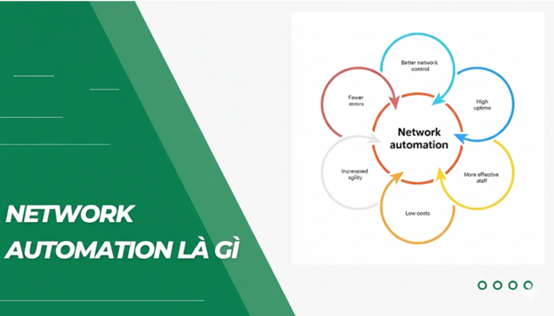
\includegraphics[width=0.7\textwidth]{image/Net_Auto.png}
            \caption{Tự động hóa mạng}
    \end{figure}

    Tự động hóa mạng (Network Automation)\cite{GeeksforGeeks-OSPF} xuất hiện như một giải pháp tất yếu để đáp ứng nhu cầu vận hành hạ tầng mạng hiệu quả, đáng tin cậy và có khả năng mở rộng cao. Thông qua việc sử dụng các công cụ lập trình và kịch bản tự động, quản trị viên mạng có thể triển khai cấu hình đồng loạt, giám sát trạng thái thiết bị theo thời gian thực, và phát hiện cũng như khắc phục sự cố một cách nhanh chóng. Điều này không chỉ giảm thiểu thời gian downtime mà còn tối ưu hóa nguồn lực nhân sự, cho phép đội ngũ IT tập trung vào các nhiệm vụ chiến lược thay vì các công việc lặp đi lặp lại.
    
    Hơn nữa, tự động hóa mạng đóng vai trò quan trọng trong việc đảm bảo tính nhất quán của cấu hình trên toàn bộ hệ thống. Khi các thay đổi được thực hiện thông qua script được kiểm thử kỹ lưỡng, khả năng xảy ra lỗi cấu hình giảm đáng kể so với việc nhập lệnh thủ công. Điều này đặc biệt quan trọng trong môi trường doanh nghiệp nơi mà sự cố mạng có thể gây ra thiệt hại tài chính lớn và ảnh hưởng nghiêm trọng đến hoạt động kinh doanh.

    

\subsection{ Mục tiêu nghiên cứu và phạm vi đề tài:}
\subsubsection{Mục tiêu nghiên cứu:}
Các mục tiêu chính, bao gồm:
\begin{itemize}
    \item \textbf{Mục tiêu học thuật:} Đề tài hướng đến việc nghiên cứu và phân tích các phương pháp tự động hóa trong quản trị hạ tầng mạng doanh nghiệp, từ đó đóng góp vào việc hệ thống hóa kiến thức về ứng dụng ngôn ngữ lập trình Python trong lĩnh vực network automation. Nghiên cứu tập trung vào việc đánh giá hiệu quả của các thư viện Python phổ biến như Netmiko, Paramiko trong việc tương tác với thiết bị mạng\cite{CloudMyLab-2025}, đồng thời xây dựng khung lý thuyết về quy trình tự động hóa từ thu thập thông tin, triển khai cấu hình đến giám sát và khôi phục hệ thống.Đề tài cũng tìm hiểu sâu về các giao thức mạng thiết yếu như VLAN, OSPF và cơ chế định tuyến động, phân tích cách thức tích hợp chúng vào một hệ thống tự động thống nhất. Thông qua việc thiết kế và triển khai mô hình thực nghiệm, nghiên cứu sẽ đưa ra các đánh giá khách quan về độ tin cậy, khả năng mở rộng và hiệu suất của giải pháp tự động hóa so với phương pháp quản trị thủ công truyền thống.
    \item \textbf{Mục tiêu kỹ thuật:}Về mặt kỹ thuật, đề tài xây dựng một hệ thống tự động hóa hoàn chỉnh trên nền tảng mô phỏng GNS3-VM\cite{GNS3-Homepage} với cấu trúc mạng gồm ba router và ba switch, mô phỏng môi trường doanh nghiệp quy mô vừa và nhỏ. Hệ thống được phát triển với các module chức năng chính bao gồm:
    Module cấu hình VLAN tự động: Triển khai phân đoạn mạng logic, cấu hình trunk port và access port theo từng yêu cầu nghiệp vụ cụ thể.
    Module định tuyến động OSPF\cite{Cisco-OSPF-7039-1}: Tự động thiết lập các thông số OSPF, quảng bá mạng và tối ưu hóa bảng định tuyến giữa các router.
    Module quản lý địa chỉ IP\cite{GeeksforGeeks-ClassfulIP}: Tự động gán và quản lý không gian địa chỉ IP trên các interface, đảm bảo tính nhất quán và tránh xung đột.
    Module thu thập thông tin thiết bị: Tự động truy vấn và lưu trữ thông tin về phiên bản IOS, cấu hình hiện hành, trạng thái interface và các metric quan trọng.
    Module phát hiện và khôi phục lỗi: Xây dựng cơ chế so sánh cấu hình thực tế với cấu hình chuẩn, tự động phát hiện sai lệch và thực hiện rollback hoặc remediation khi cần thiết.
    Module báo cáo và logging: Tự động sinh báo cáo dưới dạng CSV, TXT với đầy đủ thông tin về quá trình thực thi, kết quả và lỗi phát sinh.
    Toàn bộ hệ thống được thiết kế theo kiến trúc modular, dễ bảo trì và có khả năng mở rộng cho các chức năng nâng cao trong tương lai như tích hợp API RESTful hoặc giao diện web-based management.

    \item \textbf{Mục tiêu ứng dụng:} Về mặt ứng dụng thực tiễn, đề tài cung cấp một giải pháp cụ thể giúp các doanh nghiệp vừa và nhỏ tối ưu hóa quy trình quản trị mạng, giảm thiểu thời gian và chi phí vận hành. Hệ thống tự động hóa cho phép quản trị viên mạng triển khai hàng loạt thay đổi cấu hình trên nhiều thiết bị đồng thời, giảm đáng kể nguy cơ lỗi do con người  và rút ngắn thời gian downtime trong quá trình bảo trì.
    
    Giải pháp đặc biệt hữu ích trong các tình huống như triển khai nhanh chi nhánh mới, thay đổi cấu trúc VLAN theo yêu cầu nghiệp vụ, hoặc khôi phục hệ thống sau sự cố mạng. Khả năng tự động sinh báo cáo chi tiết giúp đáp ứng yêu cầu về kiểm toán, tuân thủ quy định  và hỗ trợ việc ra quyết định dựa trên dữ liệu.
    
    Hơn nữa, đề tài tạo ra một framework có thể tùy biến và mở rộng, cho phép doanh nghiệp điều chỉnh theo nhu cầu đặc thù của mình hoặc tích hợp vào các hệ thống quản lý tập trung (NMS) hiện có. Mô hình này cũng có thể được sử dụng làm công cụ đào tạo cho kỹ thuật viên mạng mới, giúp họ làm quen với các khái niệm network automation và Infrastructure as Code (IaC).

\end{itemize}

\subsubsection{Phạm vi đề tài:}
    Nghiên cứu được giới hạn trong môi trường mô phỏng GNS3-VM\cite{GNS3-Documentation} với thiết bị Cisco IOS, tập trung vào các giao thức và công nghệ phổ biến trong doanh nghiệp SME. Đề tài không bao gồm các khía cạnh bảo mật nâng cao, giám sát hiệu năng thời gian thực hoặc tích hợp với hệ thống cloud.

\subsection{Công nghệ sử dụng:}
    Để hiện thực hóa các mục tiêu đã đặt ra, đề tài lựa chọn và tích hợp một số công nghệ then chốt tạo thành một hệ sinh thái hoàn chỉnh cho tự động hóa mạng. Python được chọn làm ngôn ngữ lập trình chính nhờ vào tính đơn giản, dễ học và đặc biệt là hệ sinh thái thư viện phong phú trong lĩnh vực network automation. Python cung cấp khả năng xử lý chuỗi mạnh mẽ, hỗ trợ đa luồng, và có thể tích hợp dễ dàng với nhiều hệ thống khác nhau.
    
    Thư viện Netmiko đóng vai trò cốt lõi trong việc thiết lập kết nối và tương tác với các thiết bị mạng. Được xây dựng dựa trên thư viện Paramiko, Netmiko cung cấp một lớp trừu tượng cao hơn, được tối ưu hóa đặc biệt cho việc làm việc với các thiết bị network như Cisco, Juniper, Arista và nhiều nhà sản xuất khác. Thư viện này hỗ trợ nhiều phương thức kết nối an toàn thông qua SSH, cho phép gửi lệnh, nhận kết quả, và xử lý các tình huống đặc biệt như enable mode, config mode một cách tự động.
    
    Về mặt môi trường mô phỏng, GNS3-VM được sử dụng để tạo ra một môi trường lab ảo hóa hoàn chỉnh\cite{GNS3-Homepage}. GNS3 cho phép mô phỏng các thiết bị mạng thực tế với đầy đủ tính năng của Cisco IOS và các hệ điều hành mạng khác, mà không cần đến phần cứng vật lý đắt tiền. Nền tảng này cung cấp khả năng thiết kế topology linh hoạt, kết nối các thiết bị ảo với nhau, và quan trọng là cho phép các script Python kết nối đến các thiết bị này thông qua mạng IP ảo, tạo ra môi trường thử nghiệm gần giống với hệ thống thực tế.

    Sự kết hợp giữa Python, Netmiko và GNS3 tạo thành một giải pháp toàn diện, cho phép phát triển, thử nghiệm và triển khai các kịch bản tự động hóa mạng trong môi trường kiểm soát. Điều này không chỉ giảm thiểu rủi ro mà còn tạo cơ hội học hỏi và thử nghiệm các kỹ thuật mới một cách an toàn.

       
	\newpage
	
	\section*{CHƯƠNG 2 - CƠ SỞ LÝ THUYẾT}
\addcontentsline{toc}{section}{\numberline{}CHƯƠNG 2 -  CƠ SỞ LÝ THUYẾT}
	\setcounter{section}{2}
	\setcounter{subsection}{0}
	\setcounter{figure}{0}
	\setcounter{table}{0}

%---------Phân trình bày nội dung chương 2
Chương này sẽ cung cấp những kiến thức nền tảng về các công nghệ được sử dụng trong đề tài.

\subsection{Giới thiệu về Network Automation:}
    Network Automation, hay tự động hóa mạng, là quá trình sử dụng phần mềm để tự động hóa các tác vụ cấu hình, quản lý, kiểm tra và vận hành hạ tầng mạng máy tính. Thay vì phải thực hiện thủ công từng lệnh trên từng thiết bị, kỹ thuật viên có thể viết các chương trình hoặc script để thực thi hàng loạt các thao tác phức tạp trên nhiều thiết bị cùng một lúc, đảm bảo tính nhất quán và giảm thiểu sai sót.
    
    Trong mô hình truyền thống, quản trị viên mạng phải đăng nhập vào từng thiết bị thông qua console hoặc SSH, sau đó nhập các lệnh cấu hình theo cú pháp của từng nhà sản xuất. Quy trình này không chỉ tốn thời gian mà còn dễ dẫn đến các lỗi như nhầm lẫn cú pháp, quên bước, hoặc cấu hình không đồng nhất giữa các thiết bị. Network Automation giải quyết những vấn đề này bằng cách mã hóa các best practice thành code, cho phép thực thi nhanh chóng, đáng tin cậy và có thể lặp lại nhiều lần.
    
    Các lợi ích chính của Network Automation bao gồm việc tăng tốc độ triển khai cấu hình từ hàng giờ xuống còn vài phút, giảm đáng kể tỷ lệ lỗi cấu hình từ 40-60\% trong phương pháp thủ công xuống dưới 5\%, và cải thiện khả năng phản ứng với sự cố. Hơn nữa, automation cho phép thực hiện các chiến lược backup và restore cấu hình tự động, đảm bảo business continuity trong trường hợp xảy ra thảm họa. Từ góc độ vận hành, tự động hóa giúp giải phóng thời gian của đội ngũ IT để tập trung vào các dự án có giá trị cao hơn thay vì các công việc lặp đi lặp lại.
    
    Xu hướng hiện đại trong Network Automation đang chuyển từ các script đơn giản sang các framework phức tạp hơn như Ansible, SaltStack, và các giải pháp IBN. Tuy nhiên, việc nắm vững các nguyên lý cơ bản thông qua lập trình Python và các thư viện như Netmiko vẫn là nền tảng quan trọng, giúp hiểu rõ bản chất của việc tương tác với thiết bị mạng qua API và giao thức SSH


\subsection{Thư viện Netmiko và cách hoạt động:}
    Netmiko là một thư viện Python mã nguồn mở được phát triển bởi Kirk Byers, được thiết kế đặc biệt để đơn giản hóa việc kết nối SSH đến các thiết bị mạng và thực thi các lệnh trên chúng. Thư viện này được xây dựng trên nền tảng Paramiko, một implementation của giao thức SSHv2 trong Python, nhưng bổ sung thêm nhiều tính năng được tối ưu hóa cho network device.

    Về mặt kiến trúc, Netmiko hoạt động theo mô hình client-server, trong đó script Python đóng vai trò client thiết lập kết nối SSH đến thiết bị mạng (server). Quá trình kết nối bắt đầu bằng việc khởi tạo một object ConnectHandler với các tham số bao gồm device\_type (loại thiết bị như cisco\_ios, cisco\_nxos), host (địa chỉ IP hoặc hostname), username, password, và các tùy chọn khác như secret (enable password). Netmiko tự động xử lý quá trình handshake SSH, authentication, và thiết lập session\cite{Python-Automation-Book}.

    Một trong những điểm mạnh của Netmiko là khả năng tự động phát hiện và xử lý các prompt khác nhau của thiết bị. Khi một lệnh được gửi đi thông qua phương thức send\_command(), Netmiko sẽ đợi cho đến khi nhận được prompt tiếp theo từ thiết bị trước khi trả về kết quả. Điều này giải quyết vấn đề timing trong automation, vì các lệnh khác nhau có thể mất thời gian thực thi khác nhau. Thư viện cũng hỗ trợ phương thức send\_config\_set() để gửi nhiều lệnh cấu hình cùng lúc, tự động vào config mode và thoát ra sau khi hoàn thành.

    Netmiko xử lý nhiều trường hợp đặc biệt trong quá trị mạng Cisco, chẳng hạn như tự động nhập enable password khi cần, xử lý các câu hỏi xác nhận (như "Do you want to continue?"), và quản lý session timeout. Thư viện cũng hỗ trợ TextFSM, một công cụ parsing mạnh mẽ cho phép chuyển đổi output dạng text không cấu trúc thành dữ liệu có cấu trúc như dictionary hoặc list, giúp việc xử lý và phân tích kết quả trở nên dễ dàng hơn nhiều.
    
    Về bảo mật, Netmiko sử dụng SSH làm giao thức truyền tải chính, đảm bảo toàn bộ communication giữa script và thiết bị được mã hóa. Thư viện cũng hỗ trợ nhiều phương thức authentication khác nhau bao gồm password-based và key-based authentication, cho phép triển khai các chiến lược bảo mật linh hoạt. Tuy nhiên, việc quản lý credentials trong script cần được thực hiện cẩn thận, thường thông qua các biến môi trường hoặc vault management tools thay vì hard-code trực tiếp trong code\cite{NetworkJourney-Netmiko-2024}.
\subsection{Giao thức SSH trong quản trị mạng:}
    SSH là giao thức mạng mã hóa được sử dụng rộng rãi để truy cập và quản trị các hệ thống từ xa một cách an toàn. Trong quản trị mạng, SSH đã thay thế gần như hoàn toàn giao thức Telnet không bảo mật, trở thành tiêu chuẩn công nghiệp cho việc quản lý thiết bị mạng từ xa.

    SSH hoạt động trên mô hình client-server, sử dụng cổng TCP 22 mặc định. Giao thức này cung cấp ba dịch vụ bảo mật chính: authentication (xác thực danh tính), confidentiality (bảo mật dữ liệu thông qua mã hóa), và integrity (đảm bảo dữ liệu không bị thay đổi trong quá trình truyền). Quá trình thiết lập kết nối SSH diễn ra qua nhiều giai đoạn, bắt đầu với việc trao đổi phiên bản và thuật toán mã hóa, tiếp theo là key exchange để thiết lập session key, và cuối cùng là authentication của client.

    Trong bối cảnh network automation, SSH đóng vai trò then chốt vì nó cho phép script tự động kết nối đến thiết bị mà không cần sự can thiệp của con người sau khi được cấu hình đúng. SSH hỗ trợ nhiều phương thức authentication, phổ biến nhất là password-based authentication và public key authentication. Public key authentication được ưa chuộng hơn trong môi trường automation vì nó không yêu cầu truyền password qua mạng và có thể được tự động hóa hoàn toàn thông qua SSH agent hoặc key files.

    Một khía cạnh quan trọng của SSH trong automation là khả năng thiết lập session persistence và connection pooling. Thay vì phải thiết lập kết nối mới cho mỗi lệnh, SSH cho phép duy trì một session duy nhất và thực thi nhiều lệnh tuần tự, giảm overhead và tăng hiệu suất. Điều này đặc biệt quan trọng khi thực hiện cấu hình phức tạp yêu cầu nhiều bước hoặc khi phải thu thập thông tin từ nhiều thiết bị.
    
    SSH cũng cung cấp các cơ chế để xử lý timeout và connection failures, cho phép script automation có thể retry hoặc fallback sang phương án khác khi gặp vấn đề mạng. Các tính năng như keepalive packets giúp duy trì kết nối trong các session dài, tránh bị disconnect do idle timeout. Trong triển khai thực tế, việc cấu hình đúng các tham số SSH như connection timeout, banner timeout, và command timeout là rất quan trọng để đảm bảo script hoạt động ổn định trong môi trường mạng không hoàn hảo.
\subsection{VLAN, OSPF và IP Routing cơ bản:}
\subsubsection{Virtual LAN:}
    Virtual LAN (VLAN) là công nghệ cho phép phân đoạn một mạng vật lý thành nhiều mạng logic độc lập ở tầng Data Link (Layer 2) của mô hình OSI. Thay vì phải sử dụng các switch vật lý riêng biệt cho từng phòng ban hoặc nhóm người dùng, VLAN cho phép tạo ra các broadcast domain khác nhau trên cùng một hạ tầng switch vật lý, tối ưu hóa việc sử dụng thiết bị và giảm chi phí.
    
    Nguyên lý hoạt động của VLAN dựa trên việc gán tag (thẻ) cho các frame Ethernet theo chuẩn IEEE 802.1Q. Mỗi VLAN được định danh bởi một VLAN ID (VID) nằm trong khoảng từ 1 đến 4094, với VLAN 1 thường là VLAN mặc định. Khi một frame đi qua trunk port (cổng nối giữa các switch), nó được gắn thêm 4 bytes chứa thông tin VLAN ID, cho phép nhiều VLAN được truyền qua cùng một đường link vật lý. Các access port (cổng kết nối thiết bị đầu cuối) chỉ thuộc về một VLAN duy nhất và tự động gỡ bỏ tag trước khi chuyển frame đến thiết bị.
    
    VLAN mang lại nhiều lợi ích quan trọng trong quản trị mạng doanh nghiệp. Về mặt bảo mật, VLAN tạo ra sự cô lập logic giữa các nhóm người dùng, ngăn chặn việc truy cập trái phép vào các segment mạng nhạy cảm. Về hiệu năng, VLAN giúp giảm kích thước broadcast domain, hạn chế lưu lượng broadcast không cần thiết và cải thiện băng thông khả dụng. VLAN cũng tạo điều kiện cho việc triển khai QoS, cho phép ưu tiên lưu lượng của các ứng dụng quan trọng như VoIP hoặc video conferencing.
\subsubsection{Open Shortest Path First:}
    OSPF là một giao thức định tuyến động thuộc loại IGP, sử dụng thuật toán link-state để xây dựng và duy trì bảng định tuyến\cite{GeeksforGeeks-OSPF}\cite{Cloudflare-OSPF}. Khác với các giao thức distance-vector như RIP, OSPF lưu trữ toàn bộ topology của mạng và sử dụng thuật toán Dijkstra để tính toán đường đi ngắn nhất (shortest path) đến mỗi destination network.
    
    Hoạt động của OSPF bắt đầu với việc các router thiết lập neighbor relationship thông qua việc trao đổi Hello packets trên các interface được kích hoạt OSPF. Sau khi adjacency được hình thành, các router sẽ trao đổi LSAs chứa thông tin về các link trực tiếp kết nối với chúng\cite{Cisco-OSPF-7039-1}. Mỗi router xây dựng một LSDB giống hệt nhau, sau đó chạy thuật toán SPF để tính toán đường đi tốt nhất đến mỗi network, kết quả được lưu trong routing table.
    
    OSPF sử dụng khái niệm metric dựa trên cost, được tính theo công thức cost = reference bandwidth / interface bandwidth\cite{Cisco-OSPF-7039-1}. Mặc định, reference bandwidth là 100 Mbps, có nghĩa là một link FastEthernet 100Mbps có cost là 1, trong khi link Gigabit Ethernet có cost là 1 (do giá trị minimum). Metric này có thể được điều chỉnh thủ công để kiểm soát traffic engineering.
    
    Một tính năng quan trọng của OSPF là khả năng phân vùng mạng thành các area nhằm giảm overhead và tăng khả năng mở rộng\cite{GeeksforGeeks-OSPF}. Area 0 (backbone area) là area bắt buộc mà tất cả các area khác phải kết nối đến, tạo thành cấu trúc two-level hierarchy. OSPF cũng hỗ trợ các tính năng nâng cao như route summarization, stub area, và virtual link, cho phép thiết kế mạng linh hoạt và hiệu quả\cite{Cisco-OSPF-7039-1}.
\subsubsection{IP Routing cơ bản:}
    IP Routing là quá trình chuyển tiếp gói tin IP từ một mạng này sang mạng khác dựa trên địa chỉ IP đích\cite{Cloudflare-Routing}\cite{CompTIA-Routing}. Mỗi router duy trì một routing table chứa thông tin về các network đích và interface hoặc next-hop router để chuyển tiếp gói tin đến đích đó. Quá trình routing diễn ra ở tầng Network (Layer 3) của mô hình OSI và là nền tảng của hoạt động Internet toàn cầu.
    
    Routing table có thể được populate thông qua ba phương thức chính: directly connected networks (các mạng kết nối trực tiếp), static routes (được cấu hình thủ công bởi administrator), và dynamic routes (được học thông qua các giao thức định tuyến động như OSPF, EIGRP, BGP)\cite{CompTIA-Routing}. Mỗi entry trong routing table bao gồm destination network, subnet mask, next-hop IP hoặc exit interface, metric, và AD để xác định độ tin cậy của nguồn thông tin routing.
    
    Khi router nhận được một gói tin, nó thực hiện longest prefix matching để tìm entry phù hợp nhất trong routing table. Ví dụ, nếu có hai route: 192.168.1.0/24 và 192.168.1.128/25, gói tin đến 192.168.1.150 sẽ khớp với route /25 vì nó có prefix dài hơn và specific hơn. Nếu không tìm thấy route nào khớp, gói tin sẽ được chuyển đến default route (nếu có) hoặc bị drop.
    
    Trong môi trường sử dụng VLAN, routing giữa các VLAN là cần thiết vì các VLAN khác nhau thuộc các broadcast domain riêng biệt và không thể communicate trực tiếp ở Layer 2. Inter-VLAN routing có thể được thực hiện thông qua router truyền thống với các physical interface riêng cho mỗi VLAN (phương pháp router-on-a-stick sử dụng subinterface), hoặc thông qua Layer 3 switch với SVI. Phương pháp Layer 3 switch được ưa chuộng trong các mạng hiện đại vì hiệu năng cao và cấu hình đơn giản hơn.

 
	\newpage \clearpage

	%----------Chương 3
\section*{CHƯƠNG 3 - TRIỂN KHAI HỆ THỐNG}
\addcontentsline{toc}{section}{\numberline{}CHƯƠNG 3 -  XÂY DỰNG HỆ THỐNG}
\setcounter{section}{3}
\setcounter{subsection}{0}
\setcounter{figure}{0}
\setcounter{table}{0}
	
%----------Phần trình bày nội dung chương 3

\subsection{ Mô hình thiết kế hệ thống:}
Mô hình mô phỏng hệ thống  một công ty với 2 chi nhánh sử dụng 3 Router và 3 Switch.

-Sơ đồ vật lý:

    \begin{figure}[h!] % Môi trường figure
        \centering % Căn giữa hình ảnh trong cột văn bản
        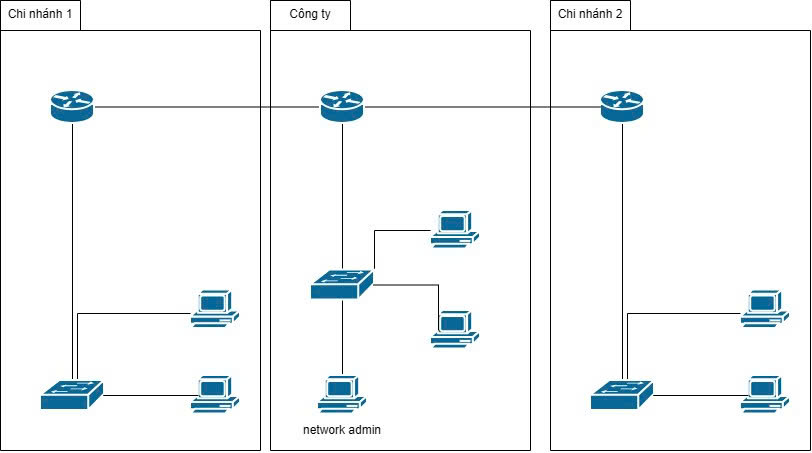
\includegraphics[width=0.7\textwidth]{image/so_do_vat_ly.jpg}
        % 

        \caption{Sơ đồ vật lý} % Chú thích hình ảnh
        \label{fig:sodo_chen_anh} % Đánh dấu để tham chiếu 
    \end{figure}
    
-Sơ đồ logic:

    \begin{figure}[h!] % Môi trường figure
        \centering % Căn giữa hình ảnh trong cột văn bản
        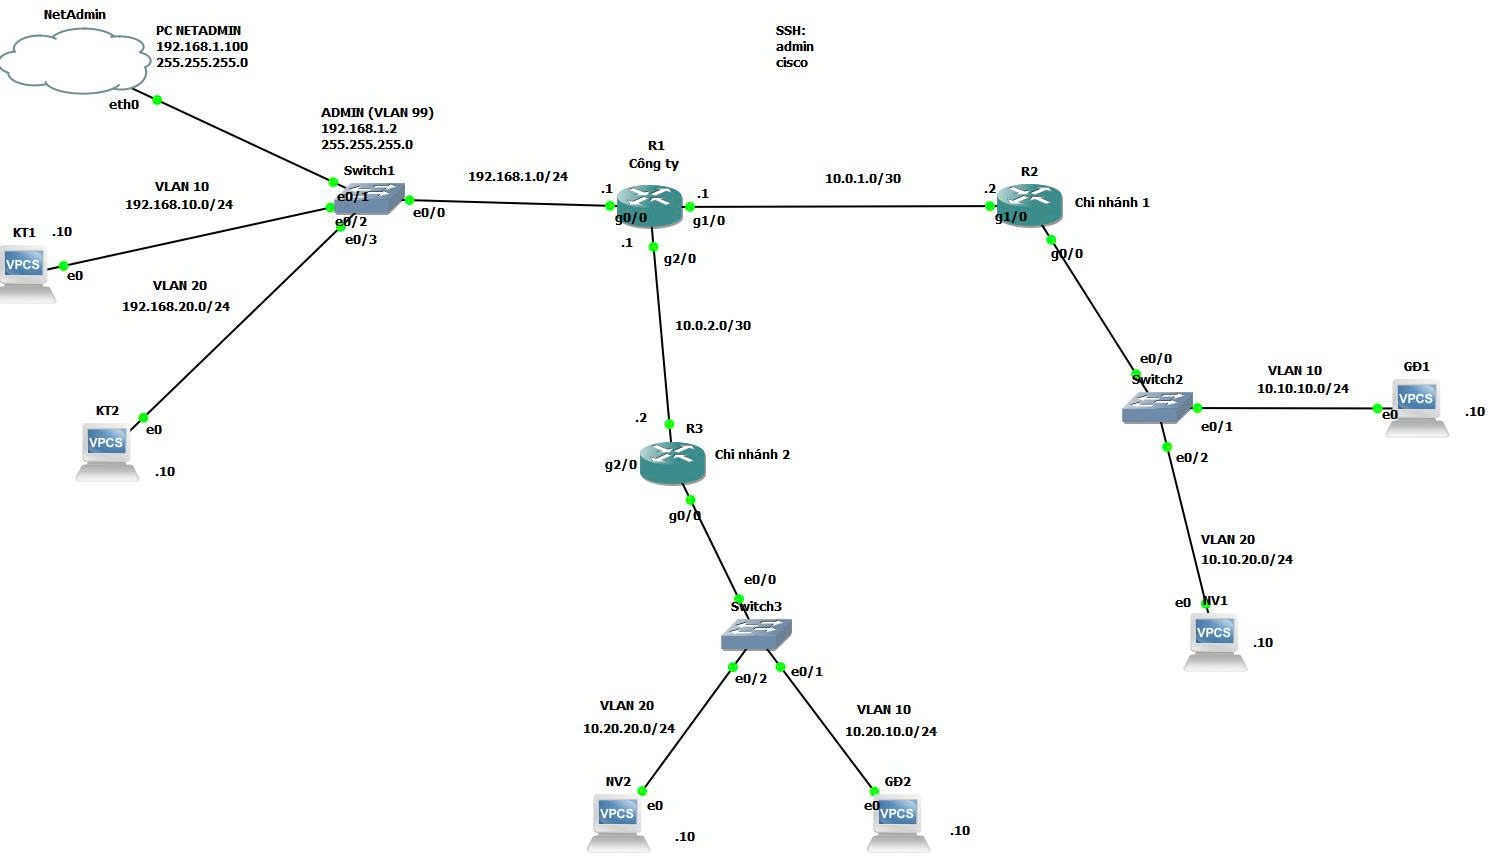
\includegraphics[width=0.7\textwidth]{image/so_do_logic.jpg}
        % 

        \caption{Sơ đồ logic} % Chú thích hình ảnh
        \label{fig:sodo_chen_anh} % Đánh dấu để tham chiếu 
    \end{figure}
    
\subsection{Thông tin IP/VLAN :}

        \label{tab:vlan_allocation}
        \begin{tabular}{|>{\centering\arraybackslash}p{0.5cm} || >{\centering\arraybackslash}p{2cm} || >{\centering\arraybackslash}p{2.5cm} || >{\centering\arraybackslash}p{3cm} || >{\centering\arraybackslash}p{4cm} |}
            \hhline{|=|=|=|=|=|}
            \textbf{No} & \textbf{Khu vực} & \textbf{VLAN Name/Label} & \textbf{Subnet/IP} & \textbf{Mô tả/Ghi chú} \\
            \hhline{|=|=|=|=|=|}
            1 & Công ty (HQ) & VLAN 10 & 192.168.10.0/24 & Phòng kỹ thuật 1 \\
            \hhline{||-||-||-||-||-||} % Chỉ kẻ ngang đơn ở giữa các dòng data
            2 & Công ty (HQ) & VLAN 20 & 192.168.20.0/24 & Phòng kỹ thuật 2 \\
            \hhline{||-||-||-||-||-||}
            3 & Công ty (HQ) & VLAN 99 & 192.168.1.2 & Phòng Network Admin \\
            \hhline{|=|=|=|=|=|} % Đường kẻ đôi ngăn cách khu vực
            4 & Chi nhánh 1 & VLAN 10 & 10.10.10.0/24 & Phòng giám đốc 1 \\
            \hhline{||-||-||-||-||-||}
            5 & Chi nhánh 1 & VLAN 20 & 10.10.20.0/24 & Phòng nhân viên 1 \\
            \hhline{|=|=|=|=|=|}
            6 & Chi nhánh 2 & VLAN 10 & 10.20.10.0/24 & Phòng giám đốc 2 \\
            \hhline{|=|=|=|=|=|}
            7 & Chi nhánh 2 & VLAN 20 & 10.20.10.0/24 & Phòng nhân viên 2 \\
            \hhline{|=|=|=|=|=|}
            8 & WAN Link 1 & R1-R2 Link & 10.0.1.0/30 & Kết nối Công ty - Chi nhánh 1 \\
            \hhline{|=|=|=|=|=|}
            9 & WAN Link 2 & R1-R3 Link & 10.0.2.0/30 & Kết nối Công ty - Chi nhánh 2 \\
            \hhline{|=|=|=|=|=|}
        \end{tabular}

\subsection{Thông tin IP Router và Thiết bị chính :}

% Bắt đầu môi trường bảng
\begin{table}[H]
    \centering 
    
    \label{tab:interface_config}
    
    % Kích thước bảng này khá rộng, nếu bị tràn lề hãy bỏ comment dòng \resizebox bên dưới và dấu } ở cuối
    % \resizebox{\textwidth}{!}{
    
    \begin{tabular}{|>{\centering\arraybackslash}p{0.5cm} || >{\centering\arraybackslash}p{2.5cm} || >{\centering\arraybackslash}p{2cm} || >{\centering\arraybackslash}p{2.8cm} || >{\centering\arraybackslash}p{3cm} || >{\centering\arraybackslash}p{3.5cm} |}
        \hhline{|=|=|=|=|=|=|}
        \textbf{No} & \textbf{Tên thiết bị} & \textbf{Interface} & \textbf{IP Address} & \textbf{Subnet Mask} & \textbf{Ghi chú} \\
        \hhline{|=|=|=|=|=|=|}
        
        % Dòng 1
        1 & PC NETADMIN & eth0 & 192.168.1.100 & 255.255.255.0 & Nối tới Switch1 \\
        \hhline{||-||-||-||-||-||-||} 
        
        % Dòng 2
        2 & \textbf{R1 (Công ty)} & g0/0 & 192.168.1.1 & 255.255.255.0 & \makecell{Gateway \\ cho mạng LAN HQ} \\
        \hhline{||-||-||-||-||-||-||}
        
        % Dòng 3
        3 & \textbf{R1 (Công ty)} & g1/0 & 10.0.1.1 & 255.255.255.252 & Nối đi R2 \\
        \hhline{||-||-||-||-||-||-||}
        
        % Dòng 4
        4 & \textbf{R1 (Công ty)} & g2/0 & 10.0.2.1 & 255.255.255.252 & Nối đi R3 \\
        \hhline{||-||-||-||-||-||-||}
        
        % Dòng 5
        5 & \textbf{PC-KT1} & eth0 & 192.168.10.10 & 255.255.255.0 & Nối tới Switch1 \\
        \hhline{||-||-||-||-||-||-||}
        
        % Dòng 6
        6 & \textbf{PC-KT2} & eth0 & 192.168.20.10 & 255.255.255.0 & \makecell{Nối tới \\ Switch1} \\
        \hhline{||-||-||-||-||-||-||}

        % Dòng 7
        7 & \textbf{R2 (Chi nhánh 1)} & g1/0 & 10.0.1.2 & 255.255.255.252 & Nối về R1 \\
        \hhline{||-||-||-||-||-||-||}

        % Dòng 8
        8 & \textbf{R2 (Chi nhánh 1)} & g0/0 & 192.168.2.1 & 255.255.255.0 & \makecell{Gateway CN1 \\ Nối tới Switch2} \\
        \hhline{||-||-||-||-||-||-||}

        % Dòng 9
        9 & \textbf{PC-GĐ1} & eth0 & 10.10.10.10 & 255.255.255.0 & Nối tới Switch2 \\
        \hhline{||-||-||-||-||-||-||}

        % Dòng 10
        10 & \textbf{PC-NV1} & eth0 & 10.10.20.10 & 255.255.255.0 & Nối tới Switch2 \\
        \hhline{||-||-||-||-||-||-||}

        % Dòng 11
        11 & \textbf{R3 (Chi nhánh 2)} & g2/0 & 10.0.2.2 & 255.255.255.252 & Nối về R1 \\
        \hhline{||-||-||-||-||-||-||}

        % Dòng 12 (Đã sửa lỗi thiếu xuống dòng ở code cũ)
        12 & \textbf{R3 (Chi nhánh 2)} & g0/0 & 192.168.3.1 & 255.255.255.0 & \makecell{Gateway CN2 \\ Nối tới R1} \\
        \hhline{||-||-||-||-||-||-||}

        % Dòng 13
        13 & \textbf{PC-GĐ2} & eth0 & 10.20.10.10 & 255.255.255.0 & Nối tới Switch3 \\
        \hhline{||-||-||-||-||-||-||}

        % Dòng 14 (Đã sửa số thứ tự từ 13 thành 14)
        14 & \textbf{PC-NV2} & eth0 & 10.20.20.10 & 255.255.255.0 & Nối tới Switch3 \\
        \hhline{|=|=|=|=|=|=|}

    \end{tabular}
    
    % } % Đóng ngoặc resizebox nếu dùng
\end{table}
    
\subsection{ Thông tin kết nối:}

    \label{tab:connection_diagram}
    
    % Cấu trúc cột: Thiết bị nguồn, Cổng nguồn, Thiết bị đích, Cổng đích, Mode/Ghi chú
    % Độ rộng cột đã được căn chỉnh để nội dung không bị quá hẹp hoặc quá rộng
    \begin{tabular}{|>{\centering\arraybackslash}p{2.5cm} || >{\centering\arraybackslash}p{1.5cm} || >{\centering\arraybackslash}p{2.5cm} || >{\centering\arraybackslash}p{1.5cm} || >{\centering\arraybackslash}p{4.5cm} |}
        \hhline{|=|=|=|=|=|}
        \textbf{Thiết bị nguồn} & \textbf{Cổng nguồn} & \textbf{Thiết bị đích} & \textbf{Cổng đích} & \textbf{Mode/Ghi chú} \\
        \hhline{|=|=|=|=|=|}
        
        NetAdmin (Cloud) & eth0 & Switch1 & e0/1 & \makecell{Tự động hoá cấu hình \\ các thiết bị} \\
        \hhline{||-||-||-||-||-||} % Kẻ ngang đơn
        
        Switch1 & e0/0 & R1 (Công ty) & g0/0 & Uplink Router \\
        \hhline{||-||-||-||-||-||}
        
        Switch1 & e0/2 & PC KT1 & e0 & VLAN 10 \\
        \hhline{||-||-||-||-||-||}
        
        Switch1 & e0/3 & PC KT2 & e0 & VLAN 20 \\
        \hhline{|=|=|=|=|=|} % Đường kẻ đôi ngăn cách khu vực
        
        R1 (Công ty) & g1/0 & R2 (Chi nhánh 1) & g1/0 & Link WAN 1 \\
        \hhline{||-||-||-||-||-||}
        
        R1 (Công ty) & g2/0 & R3 (Chi nhánh 2) & g2/0 & Link WAN 2 \\
        \hhline{|=|=|=|=|=|}
        
        R2 (Chi nhánh 1) & g0/0 & Switch2 & e0/0 & Downlink LAN \\
        \hhline{||-||-||-||-||-||}
        
        Switch2 & e0/1 & PC GD1 & e0 & VLAN 10 \\
        \hhline{||-||-||-||-||-||}
        
        Switch2 & e0/2 & PC NV1 & e0 & VLAN 20 \\
        \hhline{|=|=|=|=|=|}
        
        R3 (Chi nhánh 2) & g0/0 & Switch3 & e0/0 & Downlink LAN \\
        \hhline{||-||-||-||-||-||}
        
        Switch3 & e0/1 & PC GD2 & e0 & VLAN 10 \\
        \hhline{||-||-||-||-||-||}
        
        Switch3 & e0/2 & PC NV2 & e0 & VLAN 20 \\
        \hhline{|=|=|=|=|=|}
    \end{tabular}

	\newpage \clearpage
	
	\section*{CHƯƠNG 4 - QUY TRÌNH TỰ ĐỘNG HÓA}
\addcontentsline{toc}{section}{\numberline{}CHƯƠNG 4 -  QUY TRÌNH TỰ ĐỘNG HÓA}
\setcounter{section}{4}
\setcounter{subsection}{0}
\setcounter{figure}{0}
\setcounter{table}{0}

%-----------Phần trình bày nội dung chương 4

\subsection{Tổng quan hệ thống}
    Hệ thống tự động hóa cấu hình mạng (Network Automation System) được viết bằng Python, sử dụng thư viện Netmiko để quản lý và cấu hình các thiết bị mạng Cisco (Router và Switch). Hệ thống này cho phép tự động hóa việc cấu hình, giám sát, backup và restore cấu hình cho nhiều thiết bị mạng cùng lúc, giúp tiết kiệm thời gian và giảm thiểu sai sót so với cấu hình thủ công. 
    Các chức năng chính:
    
    \begin{itemize}
        \item Cấu hình VLAN cho Switch
        \item Cấu hình IP Interface cho Router
        \item Cấu hình OSPF routing
        \item Cấu hình Static Route
        \item Backup và Restore cấu hình
        \item Giám sát thiết bị mạng
    \end{itemize}
\subsection{Thiết lập hệ thống GNS3-VM}
\subsubsection{Yêu cầu hệ thống}
    \begin{itemize}
    \item[*] Phần cứng:
    \item CPU: Intel Core i5/i7 hỗ trợ VT-x/AMD-V
    \item RAM: 8GB (tối thiểu), 16GB (khuyến nghị)
    \item Ổ cứng: 50GB
    \item[*] Phần mềm:
    \item GNS3 GUI 2.2.46+
    \item GNS3-VM 2.2.46+
    \item VMware Workstation 17
    \item Kiểm tra VT-x: Task Manager → Performance → CPU →Virtualization.
    \item Enabled
    \end{itemize}
\subsubsection{Các bước cài đặt}
    \begin{itemize}
    \item Cài đặt GNS3-VM để hỗ trợ môi trường mô phỏng.
    \item Cài GNS3 GUI để thao tác và quản lý mô hình.
    \item Import IOS để sử dụng thiết bị Cisco trong dự án.
    \item Thiết lập kết nối mạng giữa các thành phần.
    \item Cấu hình NAT cho phép thiết bị truy cập Internet.
    \item Bật SSH để điều khiển từ xa qua script.
    \item Tạo file devices.csv lưu danh sách thiết bị.
    \item Kiểm thử quá trình tự động hóa bằng Python.
    \end{itemize}

\subsection{Kiến trúc tổng thể hệ thống tự động hoá}

    Sơ đồ kiến trúc:
        \begin{figure}[H]
            \centering
            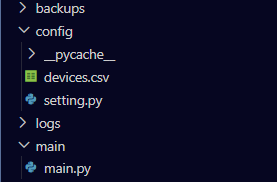
\includegraphics[width=0.7\textwidth]{image/cau_truc_code_1.png}
        \end{figure}
    
        \begin{figure}[H]
            \centering
            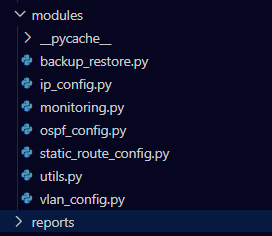
\includegraphics[width=0.7\textwidth]{image/cau_truc_code_2.png}
            \caption{Cấu trúc tổng quan}
        \end{figure}
 
\subsection{Phân tích chi tiết từng file}
\subsubsection{setting.py - File cấu hình toàn cục}
    Mục đích:
    \begin{itemize}
        \item Lưu trữ tất cả cấu hình mạng và thiết lập đường dẫn
    \end{itemize}
    Nội dung:
    \begin{itemize}
        \item Đường dẫn: BASE\_DIR, REPORTS\_DIR, LOGS\_DIR, BACKUPS\_DIR, CONFIG\_DIR.
        \item Tham số kết nối: CONNECTION\_TIMEOUT, DEVICE\_DELAY.
        \item VLAN\_CONFIGS: Cấu hình VLAN cho 3 Switch (VLAN 10, 20, 99; trunk và access ports).
        \item IP\_CONFIGS: Cấu hình IP cho 3 Router (interface, subinterface với encapsulation dot1q).
        \item OSPF\_CONFIGS: Cấu hình OSPF routing cho 3 Router (process 1, area 0).
        \item STATIC\_ROUTE\_CONFIGS: Cấu hình static route cho 3 Router.
        \item create\_directories(): Tạo các thư mục cần thiết.
    \end{itemize}
\subsubsection{utils.py - Module tiện ích chung}

    Mục đích: Cung cấp các hàm tiện ích được sử dụng chung.
    Các hàm chính:
    
    \begin{itemize}
        \item setup\_logging(): Thiết lập logging (ghi log ra file và console).
        \item load\_devices(): Đọc danh sách thiết bị từ file CSV.
        \item get\_device\_info(): Chuyển đổi thông tin thiết bị sang định dạng dict cho Netmiko.
        \item save\_results(): Lưu kết quả ra file CSV với timestamp.
        \item print\_header(): In header với tiêu đề và thời gian.
        \item print\_summary(): In tổng kết (thành công/thất bại).
        \item filter\_devices(): Lọc thiết bị theo loại hoặc hostname.
        \item confirm\_action(): Yêu cầu xác nhận từ người dùng.
        \item display\_menu(): Hiển thị menu và nhận input.
    \end{itemize}
        
\subsubsection{vlan\_config.py - Module cấu hình VLAN}
    Mục đích: Tự động cấu hình VLAN trên Switch.
    Các hàm chính:
    \begin{itemize}
        \item configure\_vlan(): Cấu hình VLAN cho một Switch.
            \begin{figure}[H]
                \centering
                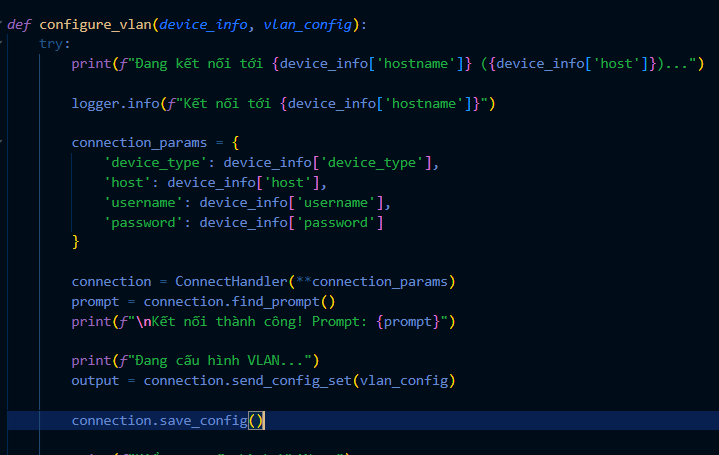
\includegraphics[width=0.7\textwidth]{image/configure_vlan_1.png}
            \end{figure}

            \begin{figure}[H]
                \centering
                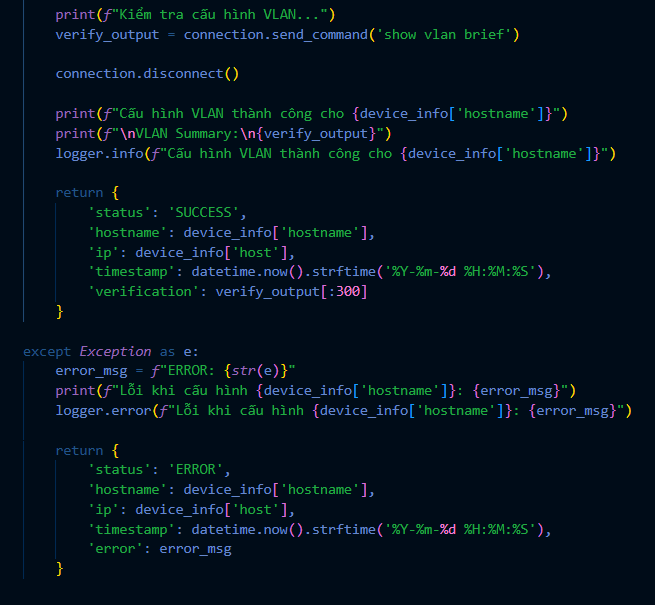
\includegraphics[width=0.7\textwidth]{image/configure_vlan_2.png}
                \caption{Cấu hình VLAN cho một Switch}
            \end{figure}
            
            
        \item configure\_all\_vlans(): Cấu hình VLAN cho tất cả Switch.
            \begin{figure}[H]
                \centering
                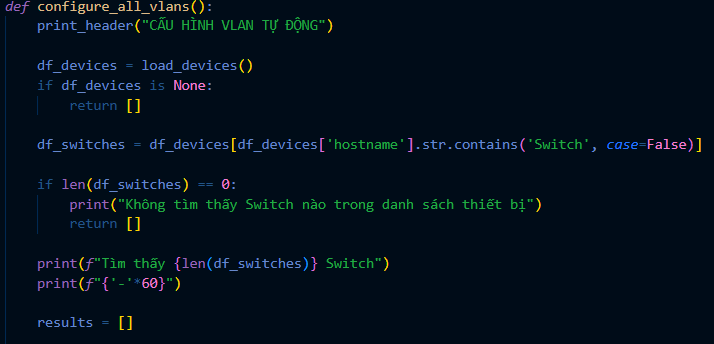
\includegraphics[width=0.7\textwidth]{image/cf_a_vlan_1.png}
            \end{figure}

            \begin{figure}[H]
                \centering
                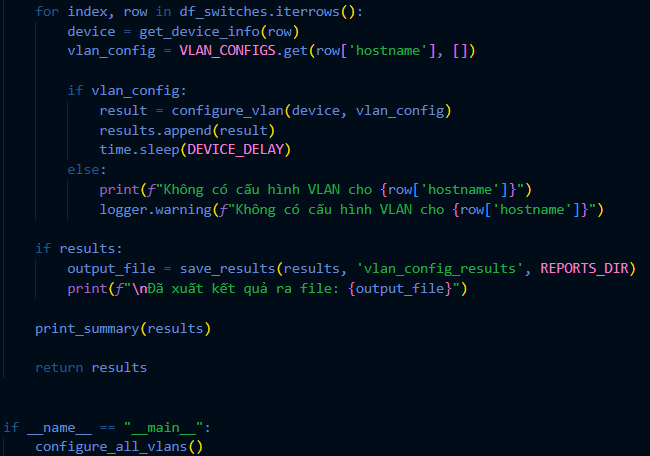
\includegraphics[width=0.7\textwidth]{image/cf_a_vlan_2.png}
                \caption{Cấu hình VLAN cho tất cả Switch}
            \end{figure}         
    \end{itemize}    
    
    \_Ý nghĩa: 
    \begin{itemize}
        \item Tạo VLAN.
        \item Cấu hình trunk port và access port.
        \item Verify bằng show vlan brief.
    \end{itemize}
\subsubsection{ip\_config.py - Module cấu hình IP Interface}
    Mục đích:Tự động cấu hình địa chỉ IP cho các interface trên Router.
    Các hàm chính:
    \begin{itemize}
        \item  configure\_ip\_interface():Cấu hình IP cho một Router.
            \begin{figure}[H]
                \centering
                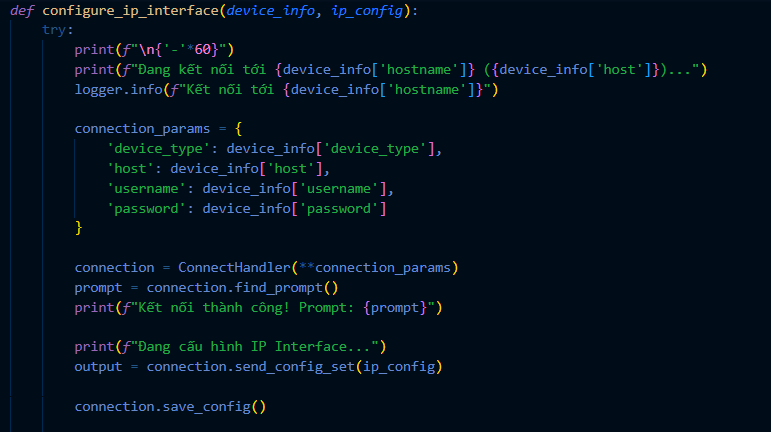
\includegraphics[width=0.7\textwidth]{image/cf_ip_if_1.png}
            \end{figure}

            \begin{figure}[H]
                \centering
                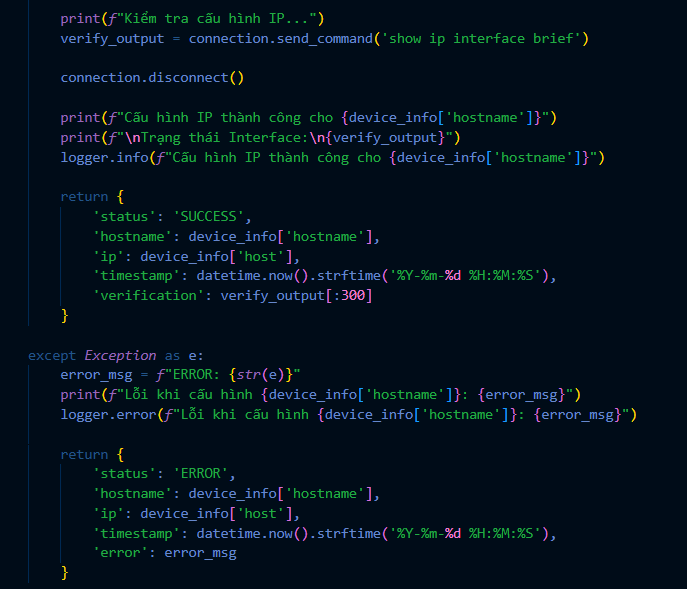
\includegraphics[width=0.7\textwidth]{image/cf_ip_if_2.png}
                \caption{Cấu hình IP cho interface trên Router}
            \end{figure}

            
        \item configure\_all\_ip\_interfaces():Áp dụng cấu hình IP cho tất cả Router.
            \begin{figure}[H]
                \centering
                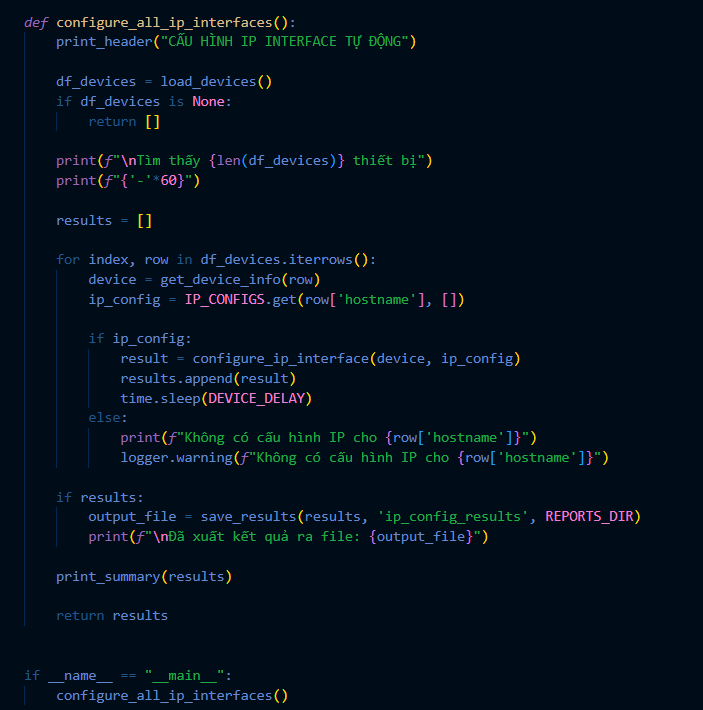
\includegraphics[width=0.5\textwidth]{image/cf_a_ip_if.png}
                \caption{Cấu hình IP cho tất cả interface trên Router}
            \end{figure}
    \end{itemize}

    \_Ý nghĩa:
    \begin{itemize}
        \item  Kết nối đến Router.
        \item  Gửi danh sách lệnh cấu hình IP.
        \item  Lưu cấu hình (write memory).
        \item  Verify bằng lệnh show ip interface brief.
    \end{itemize}
        
\subsubsection{ospf\_config.py - Module cấu hình OSPF}
    Mục đích: Tự động cấu hình giao thức định tuyến OSPF
    Các hàm chính:
    \begin{itemize}
        \item configure\_ospf(): Cấu hình OSPF cho một Router.
            \begin{figure}[H]
                \centering
                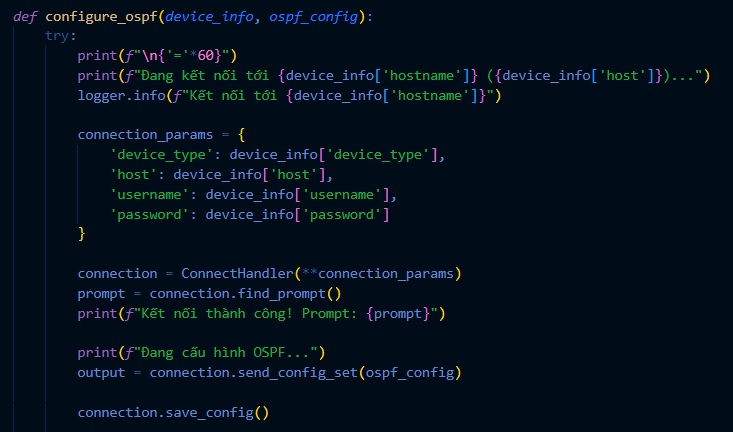
\includegraphics[width=0.7\textwidth]{image/cf_ospf_1.png}
            \end{figure}

            \begin{figure}[H]
                \centering
                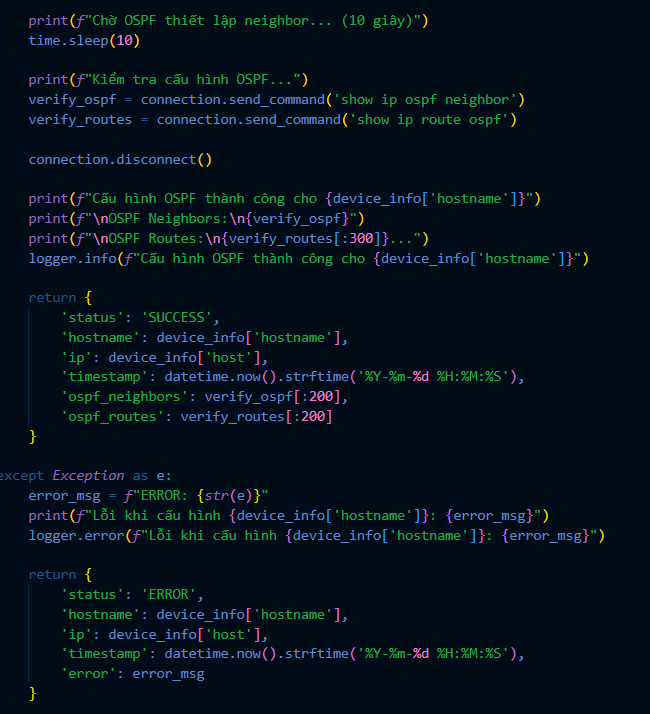
\includegraphics[width=0.7\textwidth]{image/cf_ospf_2.png}
                \caption{Cấu hình IP cho tất cả interface trên Router}
            \end{figure}

        \item configure\_all\_ospf(): Cấu hình OSPF cho tất cả Router.
            \begin{figure}[H]
                \centering
                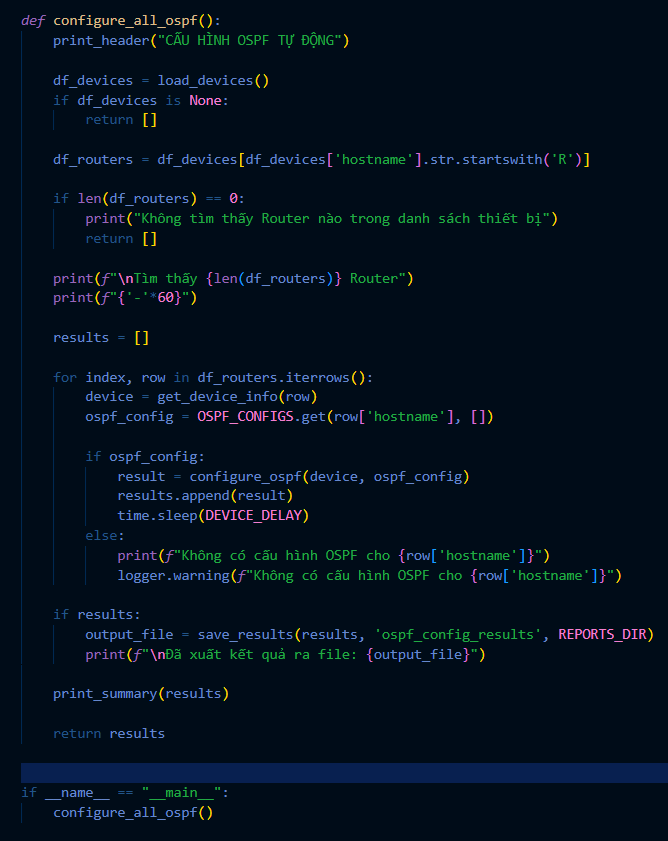
\includegraphics[width=0.7\textwidth]{image/cf_a_ospf.png}
                \caption{Cấu hình IP cho tất cả interface trên Router}
            \end{figure}
    \end{itemize}
    \_Ý nghĩa:
    \begin{itemize}
        \item Áp dụng cấu hình OSPF (router-id, network statements)
        \item Chờ 10 giây để OSPF neighbor thiết lập
        \item Verify bằng show ip ospf neighbor và show ip route ospf
    \end{itemize}
    

\subsubsection{static\_route\_config.py - Module cấu hình Static Route}
    Mục đích:Tự động cấu hình static route (thay thế OSPF nếu cần).
    Các hàm chính:
    \begin{itemize}
        \item configure\_static\_route():Cấu hình static route cho một Router.
        \begin{figure}[H]
                \centering
                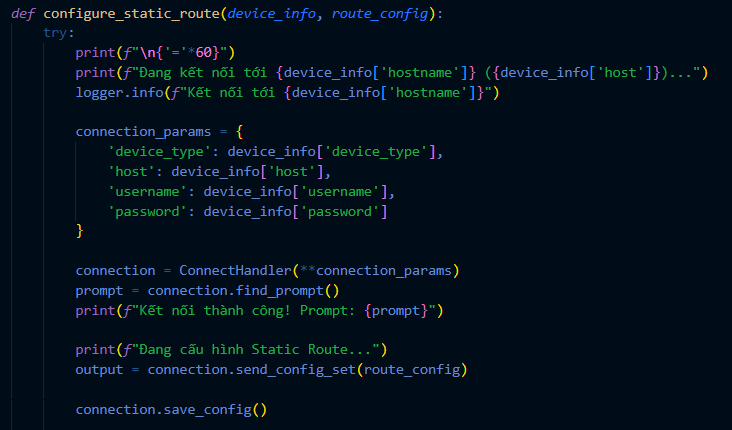
\includegraphics[width=0.7\textwidth]{image/cf_st_1.png}
                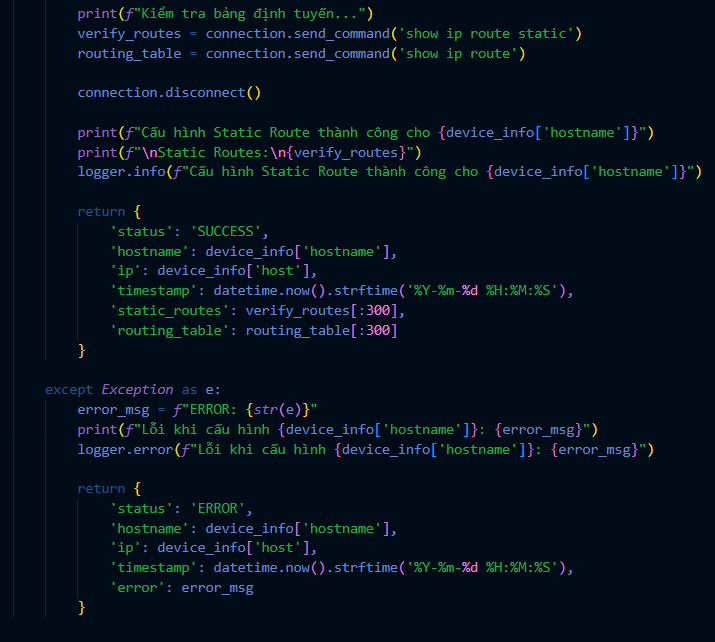
\includegraphics[width=0.7\textwidth]{image/cf_st_2.png}
                \caption{Cấu hình định tuyến tĩnh cho một Router}
        \end{figure}
        
        \item configure\_all\_static\_routes():  Cấu hình static route cho tất cả Router.
        \begin{figure}[H]
                \centering
                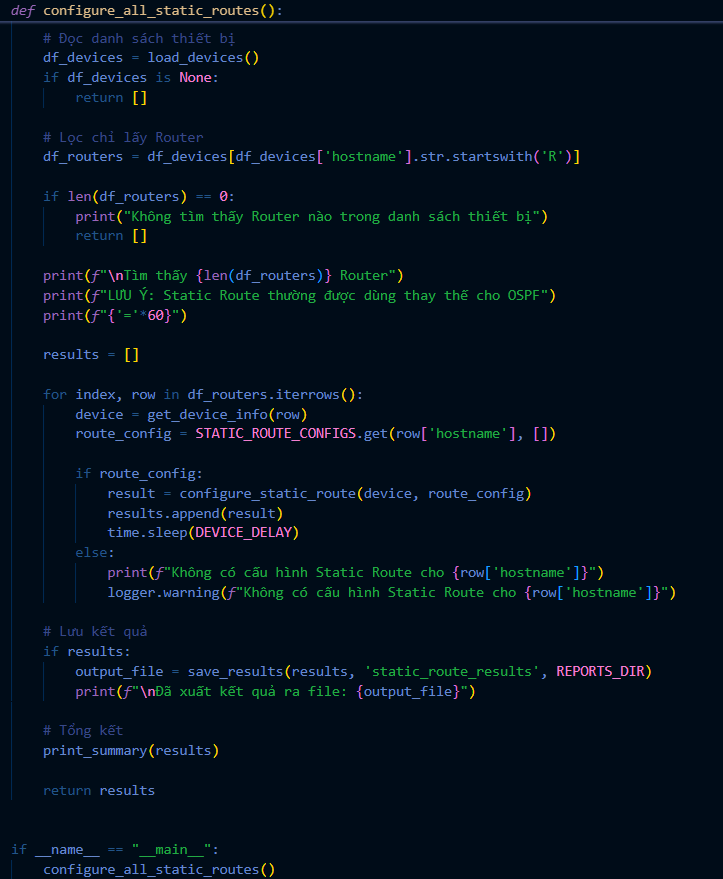
\includegraphics[width=0.7\textwidth]{image/cf_a_st.png}
                \caption{Cấu hình định tuyến tĩnh cho tất cả Router}
        \end{figure}
        
    \end{itemize}
    \_Ý nghĩa:
    \begin{itemize}
        \item Áp dụng các lệnh ip route.
        \item Verify bằng show ip route static.
    \end{itemize}


\subsubsection{backup\_restore.py - Module Backup \& Restore}
    Mục đích:Quản lý backup và khôi phục cấu hình thiết bị
    Các hàm chính:
    \begin{itemize}
        \item backup\_config():Backup cấu hình một thiết bị (lấy running-config).
        \begin{figure}[H]
                \centering
                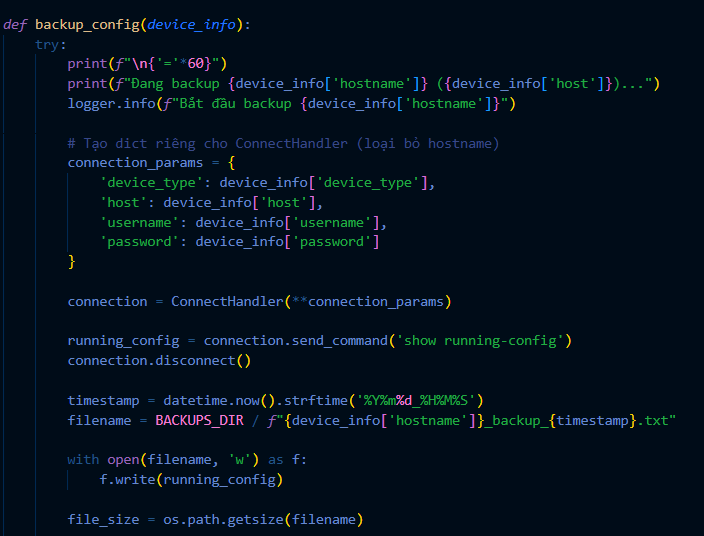
\includegraphics[width=0.7\textwidth]{image/bu_cf_1.png}
                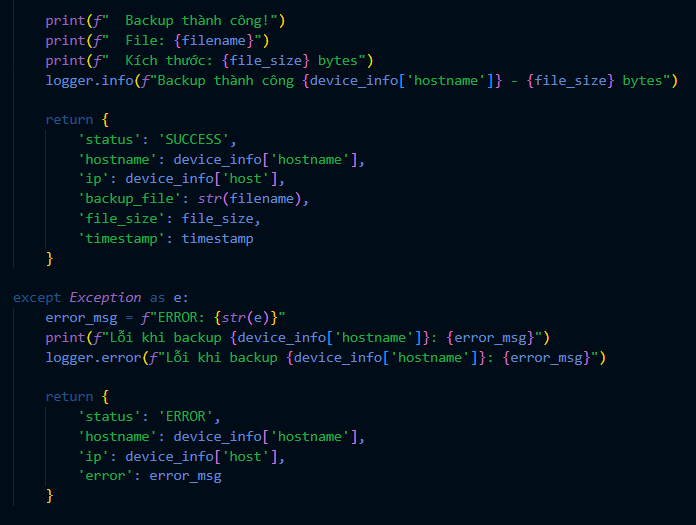
\includegraphics[width=0.7\textwidth]{image/bu_cf_2.png}
                \caption{Cấu hình backup cho một thiết bị}
        \end{figure}
        \item backup\_all\_devices():Backup tất cả thiết bị trong danh sách.
        \begin{figure}[H]
                \centering
                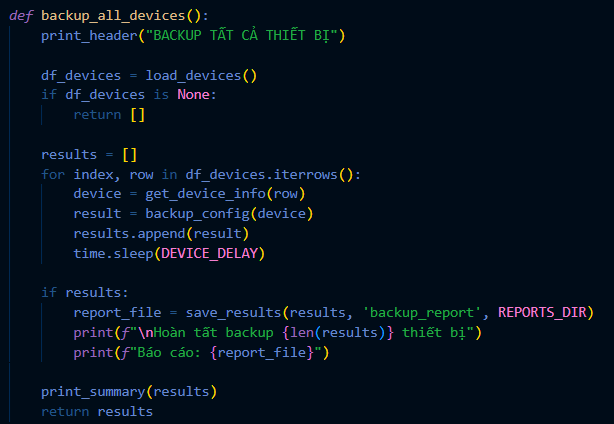
\includegraphics[width=0.7\textwidth]{image/bu_a_cf.png}
                \caption{Cấu hình backup cho tất cả thiết bị}
        \end{figure}
        \item restore\_config():Restore cấu hình từ file backup.
            \begin{figure}[H]
                \centering
                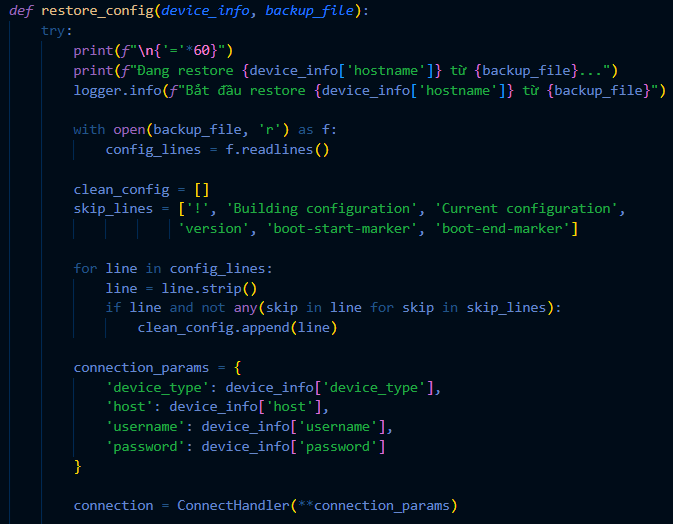
\includegraphics[width=0.7\textwidth]{image/rs_cf_1.png}
            \end{figure}

            \begin{figure}[H]
                \centering
                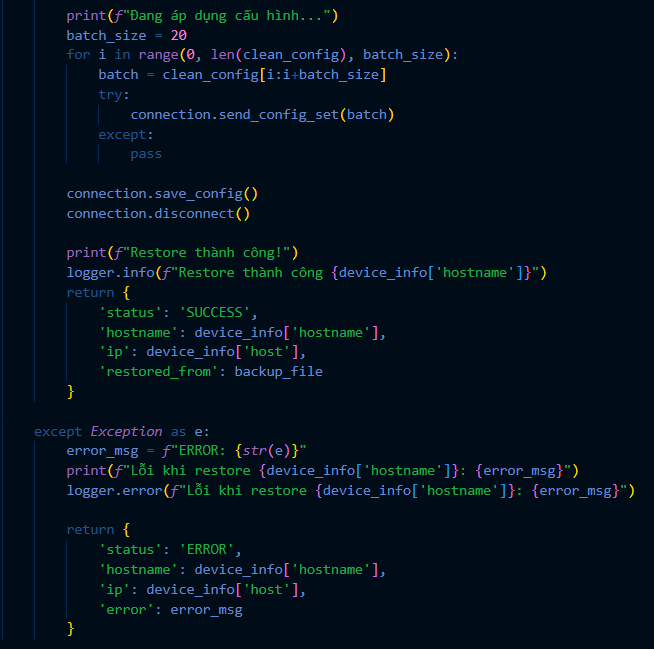
\includegraphics[width=0.7\textwidth]{image/rs_cf_2.png}
                \caption{Cấu hình lưu trữ}
            \end{figure}
            
        \item restore\_device():Cho phép chọn thiết bị và file backup để restore.
        \begin{figure}[H]
                \centering
                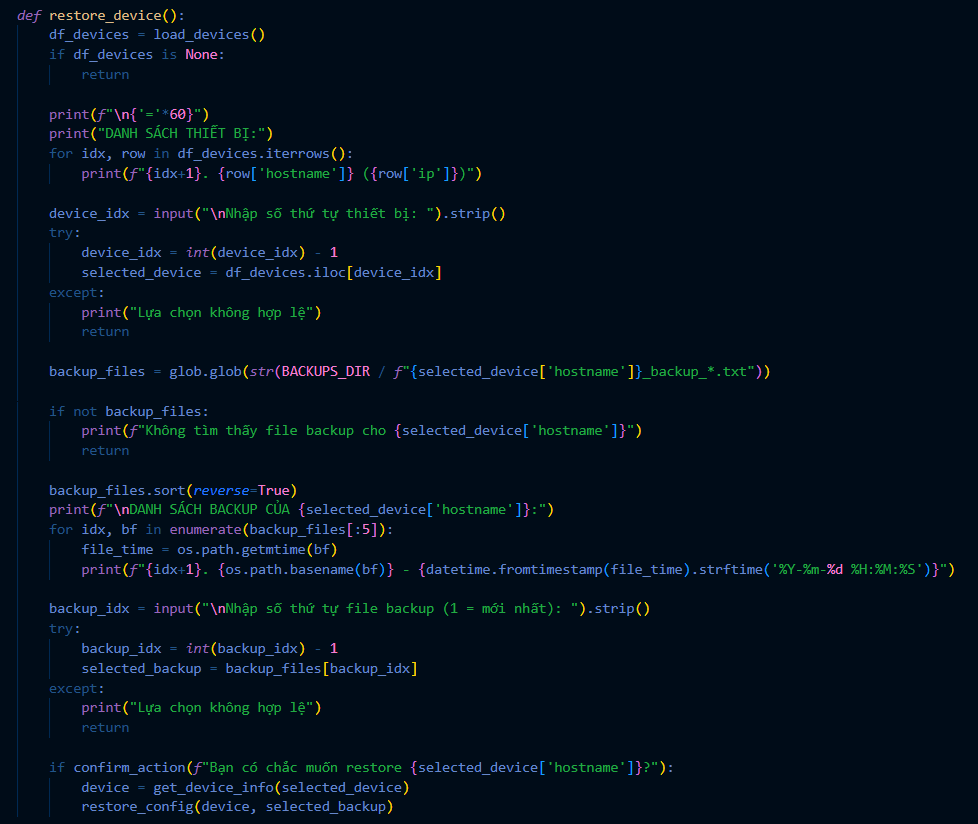
\includegraphics[width=0.7\textwidth]{image/rs_dv.png}
                \caption{Cấu hình lưu trữ thiết bị}
        \end{figure}
        \item simulate\_and\_restore():Mô phỏng lỗi (xóa subinterface) và tự động khôi phục.
        \begin{figure}[H]
                \centering
                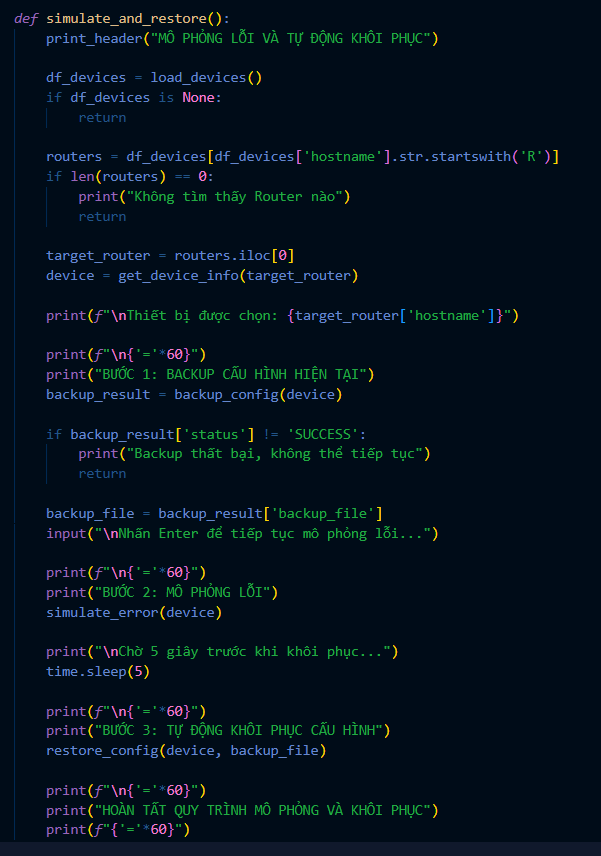
\includegraphics[width=0.7\textwidth]{image/sml_&_rs.png}
                \caption{Cấu hình mô phỏng lỗi và lưu trữ}
        \end{figure}
        \item list\_backups():Hiển thị danh sách các file backup.
        \begin{figure}[H]
                \centering
                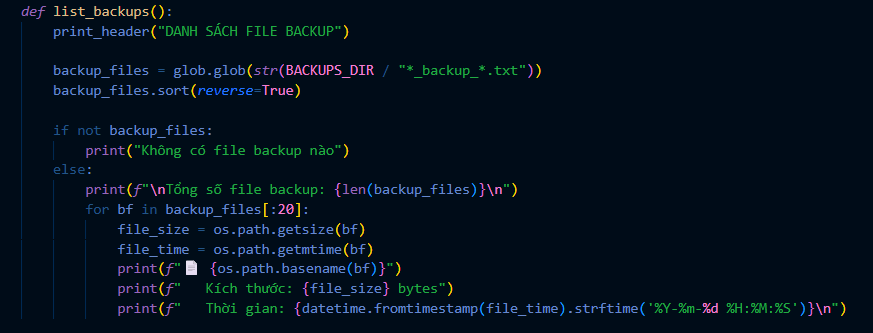
\includegraphics[width=0.7\textwidth]{image/l_bu.png}
                \caption{Cấu hình hiển thị danh sách backup}
        \end{figure}
        \item simulate\_error():Tạo lỗi giả lập bằng cách xóa cấu hình subinterface.
        \begin{figure}[H]
                \centering
                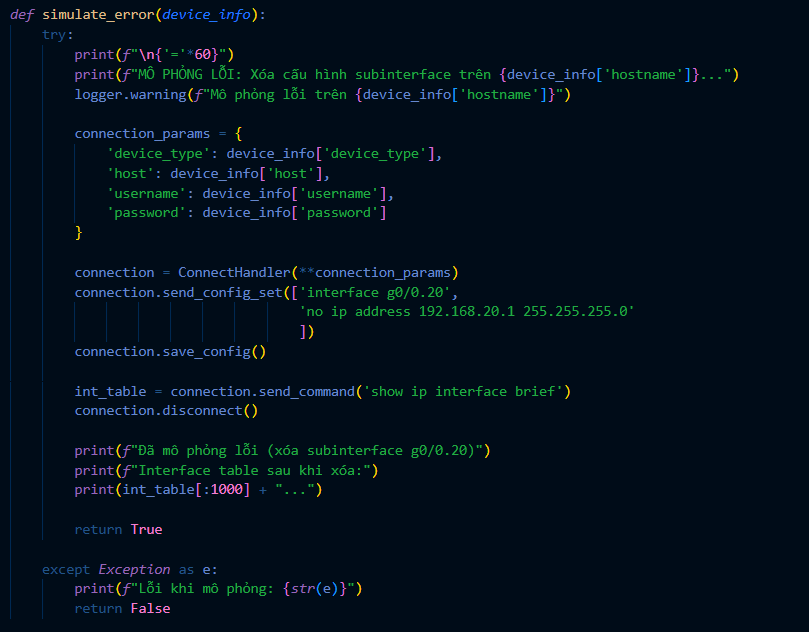
\includegraphics[width=0.7\textwidth]{image/sml_e.png}
                \caption{Cấu hình giả lập lỗi}
        \end{figure}
    \end{itemize}

\subsubsection{monitoring.py - Module giám sát thiết bị}
    Mục đích:Giám sát và kiểm tra trạng thái thiết bị mạng.
    Các hàm chính:
    \begin{itemize}
        \item check\_device\_connectivity(): Kiểm tra kết nối đến các thiết bị, đo response time.
        \begin{figure}[H]
                \centering
                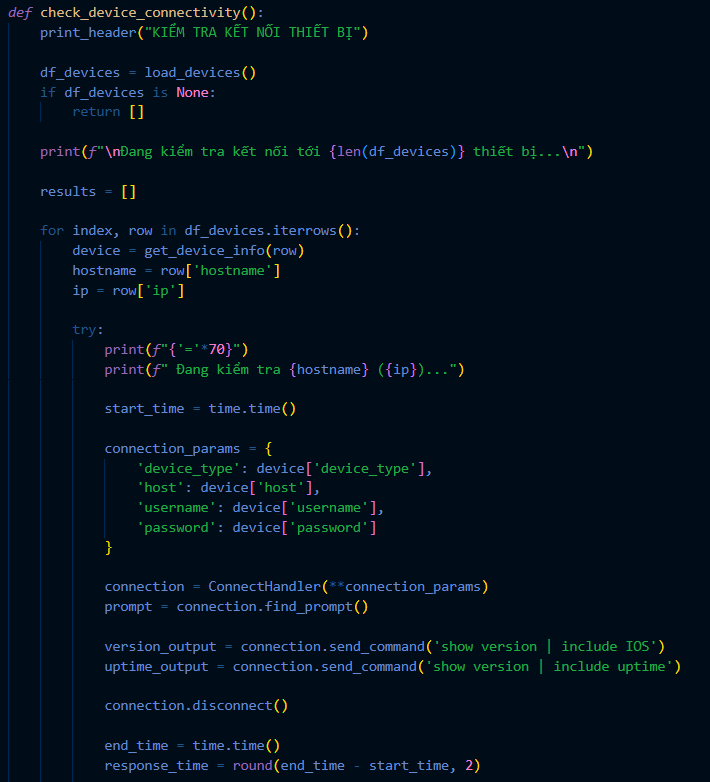
\includegraphics[width=0.7\textwidth]{image/ch_d_co_1.png}
        \end{figure}
        
        \begin{figure}[H]
                \centering
                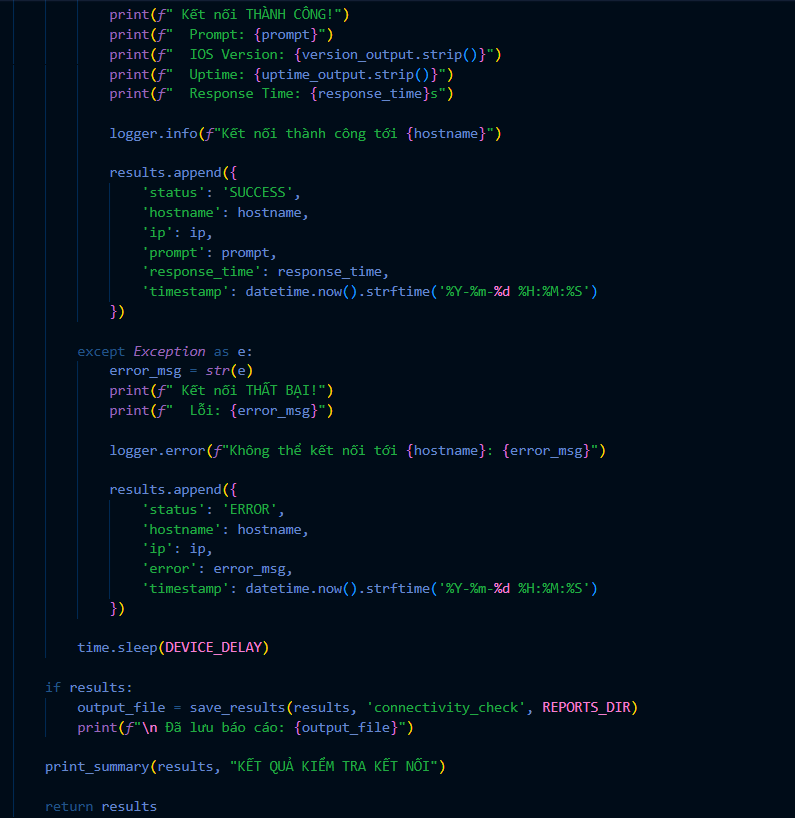
\includegraphics[width=0.7\textwidth]{image/ch_d_co_2.png}
                \caption{Cấu hình kiểm tra kết nối cho các thiết bị}
        \end{figure}
               
        \item show\_interface\_status(): Hiển thị trạng thái interface (up/down).
        \begin{figure}[H]
                \centering
                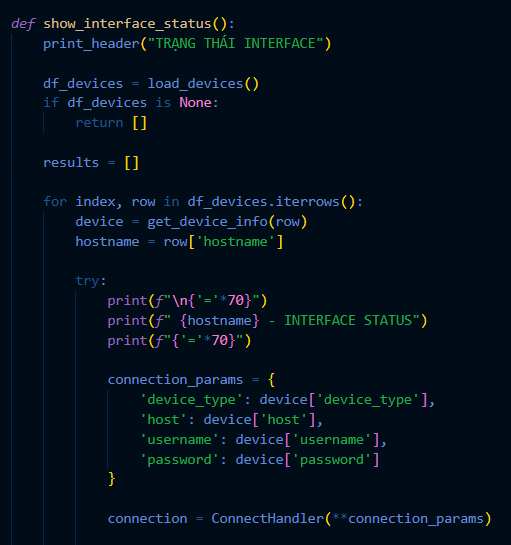
\includegraphics[width=0.7\textwidth]{image/sh_if_ st_1.png}
                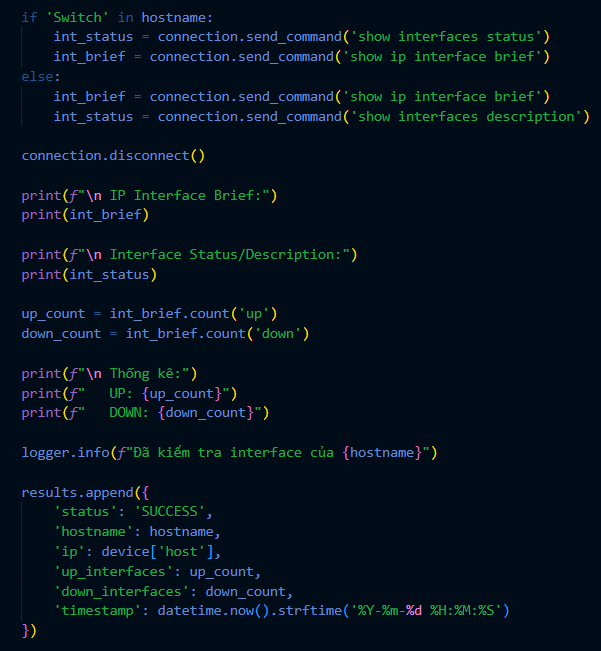
\includegraphics[width=0.7\textwidth]{image/sh_if_st_2.png}
                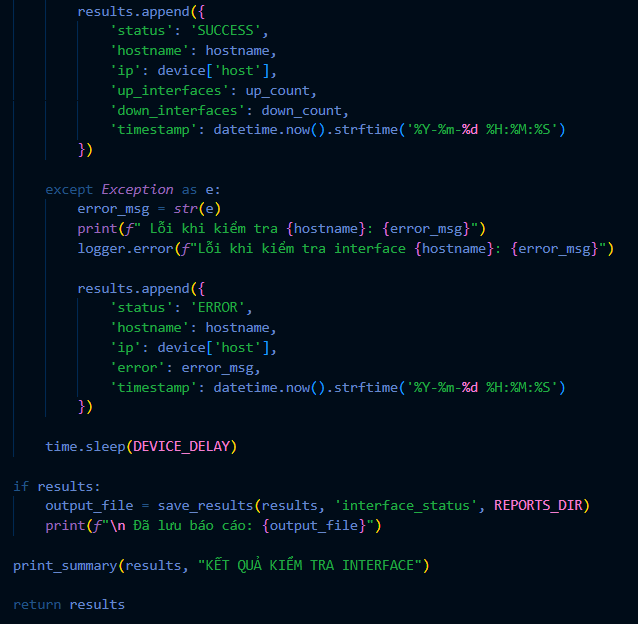
\includegraphics[width=0.7\textwidth]{image/sh_if_st_3.png}
                \caption{Cấu hình hiển thị trạng thái interface}
        \end{figure}
        \item show\_routing\_table(): Xem bảng định tuyến của Router.
        \begin{figure}[H]
                \centering
                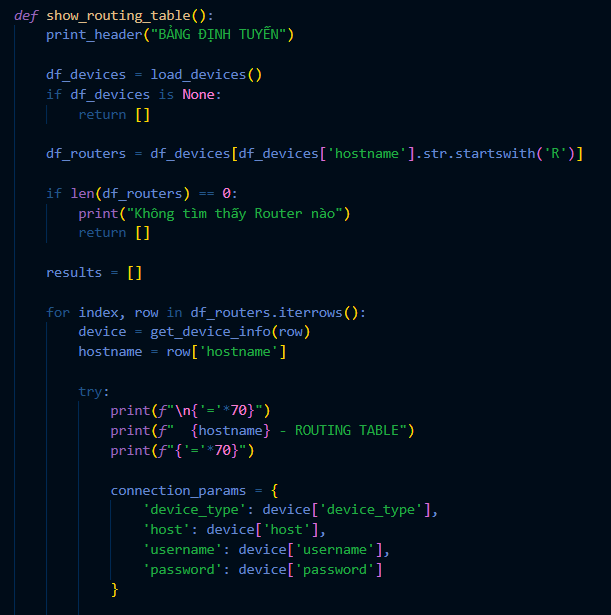
\includegraphics[width=0.7\textwidth]{image/sh_to_tb_1.png}
        \end{figure}

        \begin{figure}[H]
                \centering
                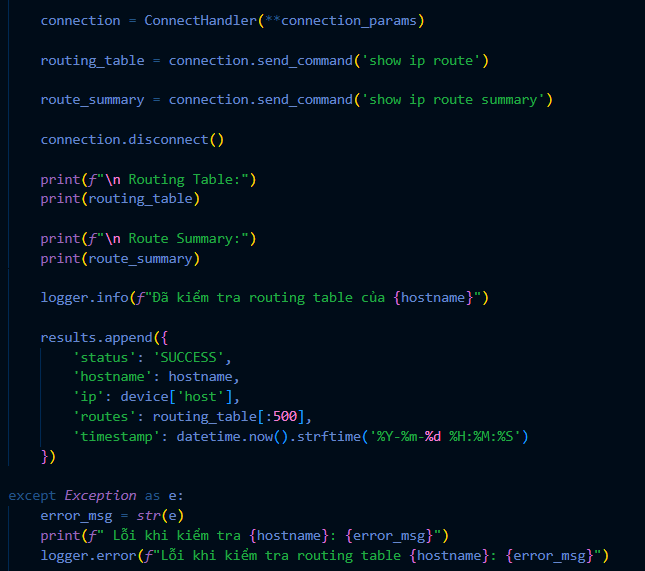
\includegraphics[width=0.7\textwidth]{image/sh_to_tb_2.png}
        \end{figure}

         \begin{figure}[H]
                \centering
                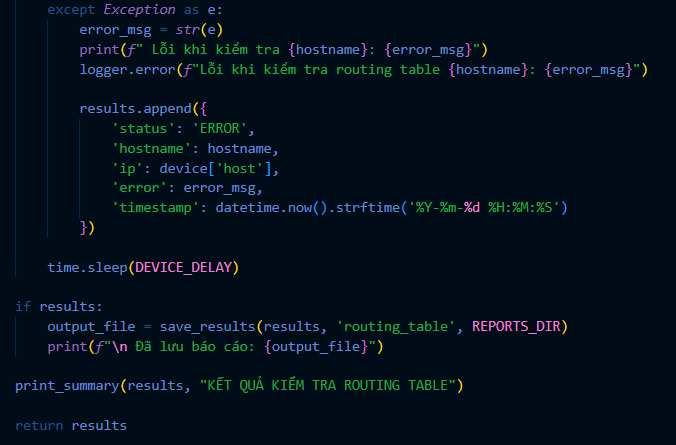
\includegraphics[width=0.7\textwidth]{image/sh_ro_tb_3.png}
                \caption{Cấu hình hiển thị định tuyến của Router}
        \end{figure}

        
        \item show\_vlan\_info(): Xem thông tin VLAN trên Switch.
        \begin{figure}[H]
                \centering
                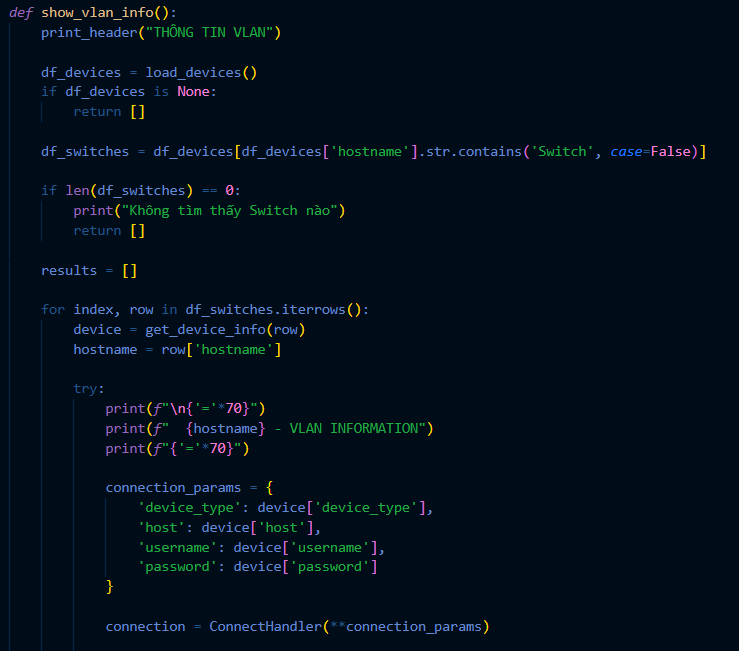
\includegraphics[width=0.7\textwidth]{image/sh_vl_i_1.png}
                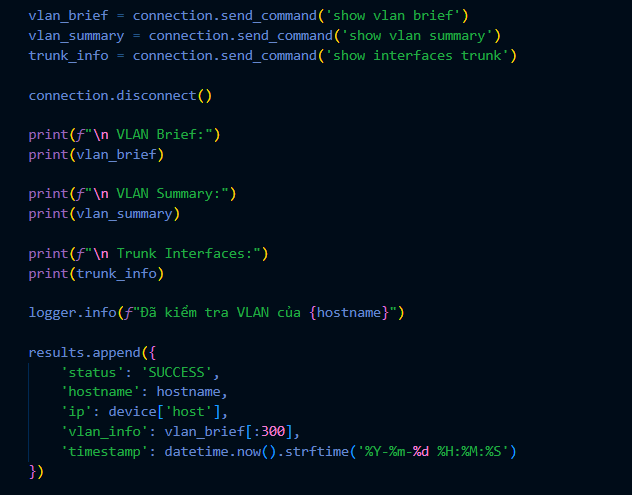
\includegraphics[width=0.7\textwidth]{image/sh_vl_i_2.png}
        \end{figure}

        \begin{figure}[H]
                \centering
                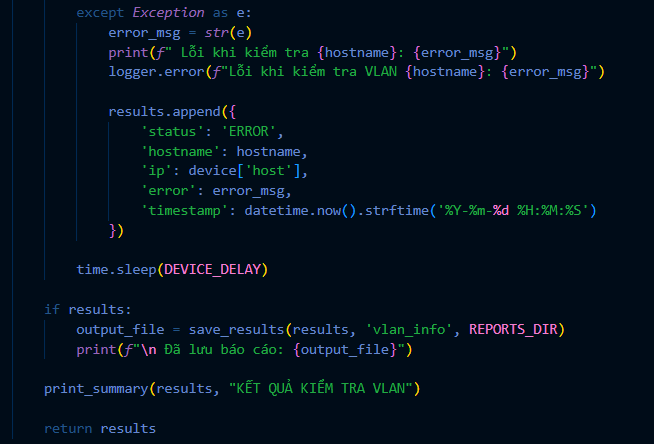
\includegraphics[width=0.7\textwidth]{image/sh_vl_i_3.png}
                \caption{Cấu hình hiển thị VLAN trên Switch}
        \end{figure}
        
        \item show\_ospf\_status(): Xem trạng thái OSPF (neighbors, database).
        \begin{figure}[H]
                \centering
                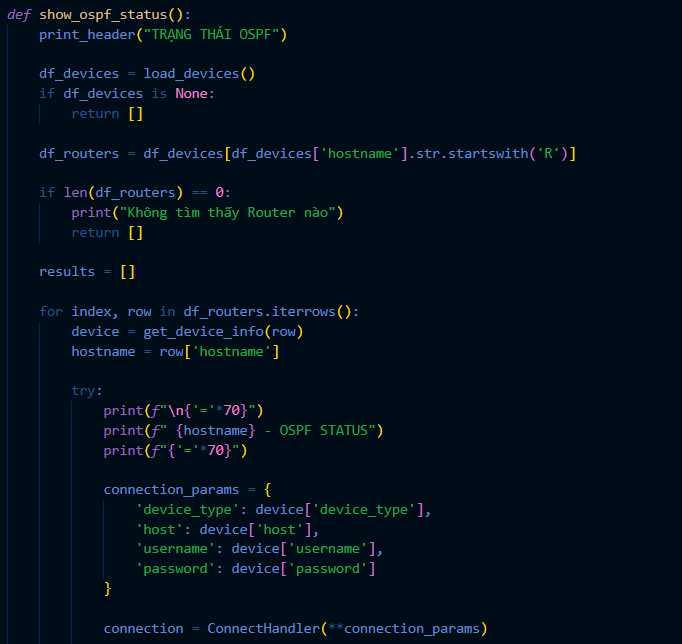
\includegraphics[width=0.7\textwidth]{image/sh_ospf_st_1.png}
        \end{figure}

        \begin{figure}[H]
                \centering
                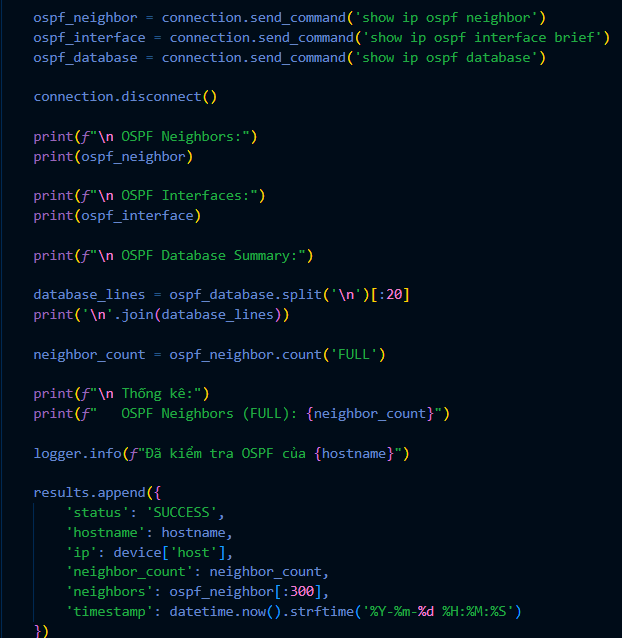
\includegraphics[width=0.7\textwidth]{image/sh_ospf_st_2.png}
        \end{figure}

        \begin{figure}[H]
                \centering
                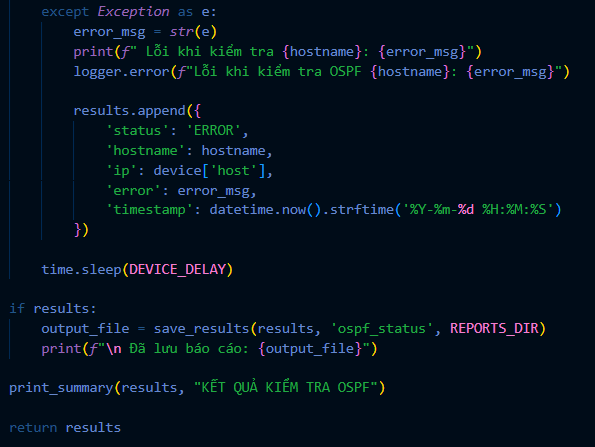
\includegraphics[width=0.7\textwidth]{image/sh_ospf_st_3.png}
                \caption{Cấu hình hiển thị trạng thái OSPF}
        \end{figure}
        
        \item monitor\_all\_devices(): Giám sát toàn diện (chạy tất cả các kiểm tra trên).
        \begin{figure}[H]
                \centering
                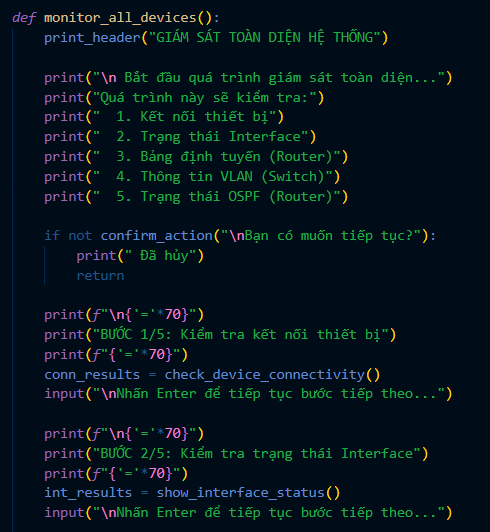
\includegraphics[width=0.7\textwidth]{image/mn_a_d_1.png}
        \end{figure}

        \begin{figure}[H]
                \centering
                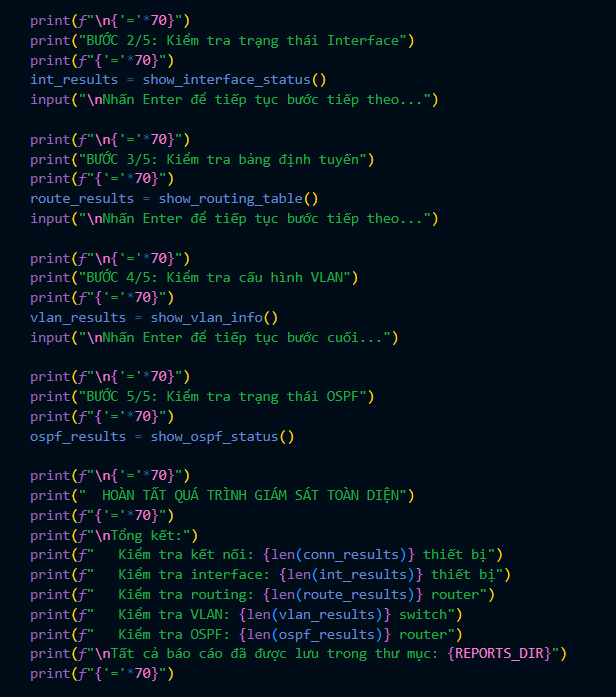
\includegraphics[width=0.7\textwidth]{image/mn_a_d_2.png}
                \caption{Cấu hình định giám sát toàn diện}
        \end{figure}
        
        \item monitoring\_menu(): Menu cho các chức năng giám sát.
        \begin{figure}[H]
                \centering
                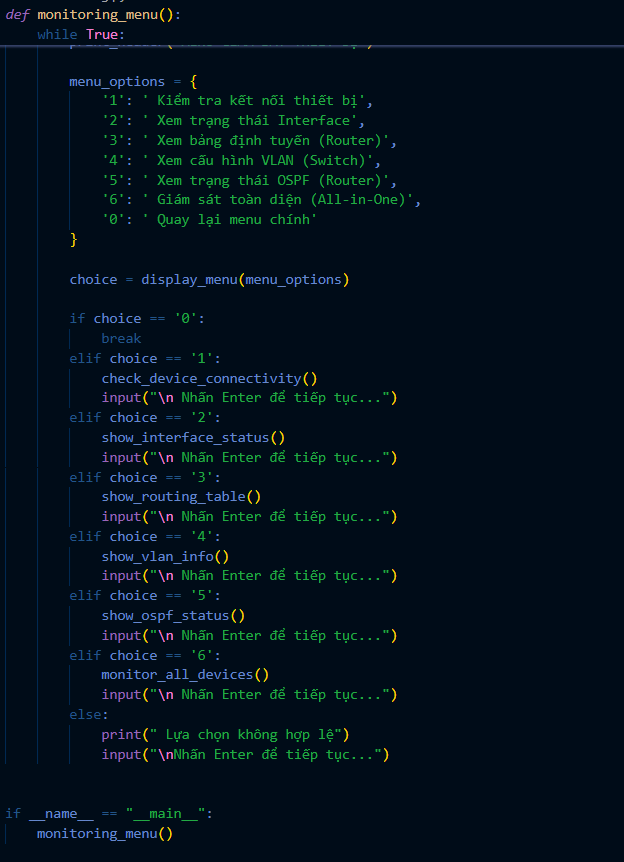
\includegraphics[width=0.7\textwidth]{image/mn_menu.png}
                \caption{Danh sách của các chức năng giám sát}
        \end{figure}
    \end{itemize}

\subsubsection{main.py - File chính của chương trình}
    Mục đích:Chạy toàn bộ các module, cung cấp giao diện menu cho người dung
    Các chức năng chính:
    \begin{itemize}
        \item show\_welcome():Hiển thị màn hình chào mừng.
        
        \begin{figure}[H]
                \centering
                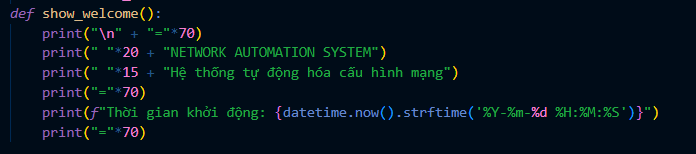
\includegraphics[width=0.7\textwidth]{image/sh_welcome.png}
                \caption{Cấu hình hiển thị chào mừng}
        \end{figure}
        
        \item configuration\_menu():Menu cấu hình thiết bị (VLAN, IP, OSPF, Static Route).
        
        \begin{figure}[H]
                \centering
                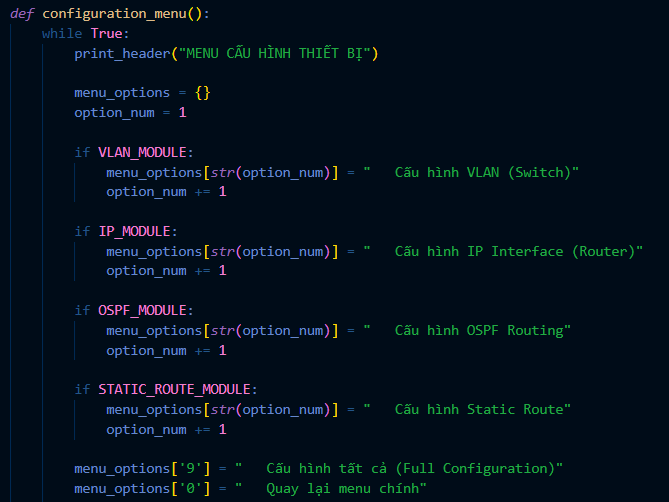
\includegraphics[width=0.7\textwidth]{image/cf_menu_1.png}
        \end{figure}

        \begin{figure}[H]
                \centering
                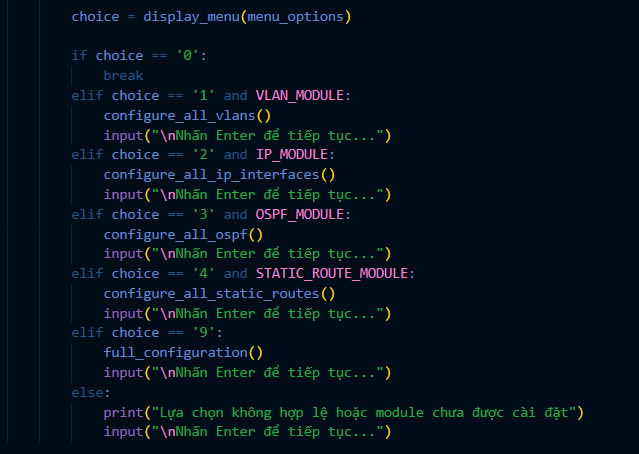
\includegraphics[width=0.7\textwidth]{image/cf_menu_2.png}
                \caption{Cấu hình hiển thị danh sách}
        \end{figure}
          
        \item backup\_restore\_menu():Menu backup và restore cấu hình.
        
        \begin{figure}[H]
                \centering
                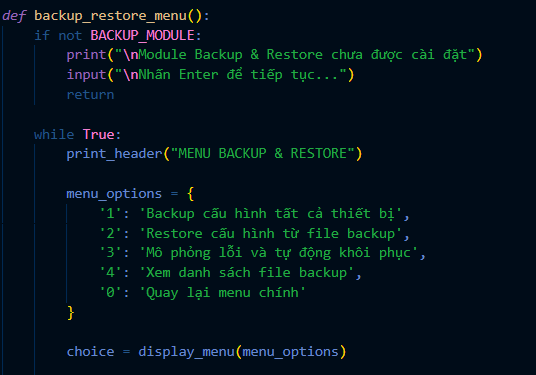
\includegraphics[width=0.7\textwidth]{image/bu_rs_menu_1.png}
        \end{figure}
        
        \begin{figure}[H]
                \centering
                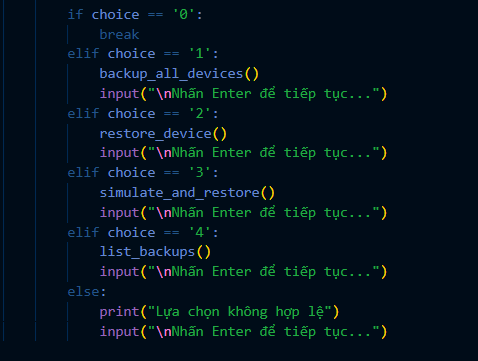
\includegraphics[width=0.7\textwidth]{image/bu_rs_menu_2.png}
                \caption{Cấu hình danh sách lưu trữ và sao lưu}
        \end{figure}
        
        \item monitoring\_menu():Menu giám sát thiết bị.
        
         \begin{figure}[H]
                \centering
                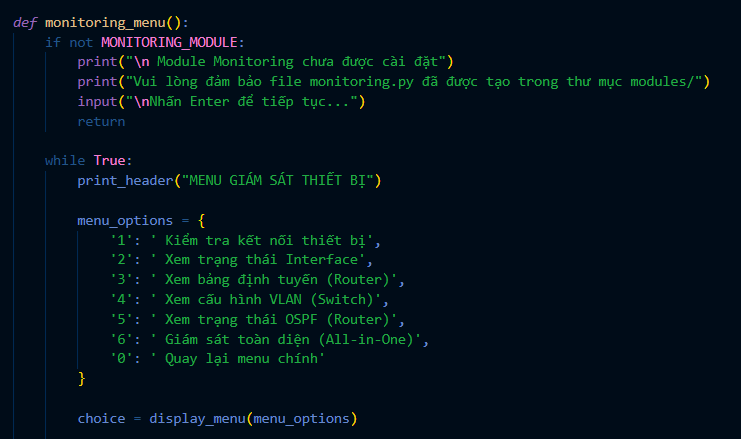
\includegraphics[width=0.7\textwidth]{image/mn_menu_1.png}
        \end{figure}

        \begin{figure}[H]
                \centering
                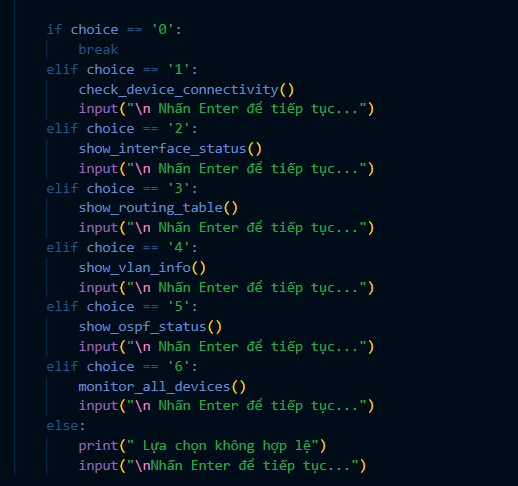
\includegraphics[width=0.7\textwidth]{image/mn_menu_2.png}
                \caption{Cấu hình danh sách giám sát thiết bị}
        \end{figure}
        
        \item full\_configuration():Thực hiện cấu hình đầy đủ toàn bộ hệ thống theo 4 bước.

        \begin{figure}[H]
                \centering
                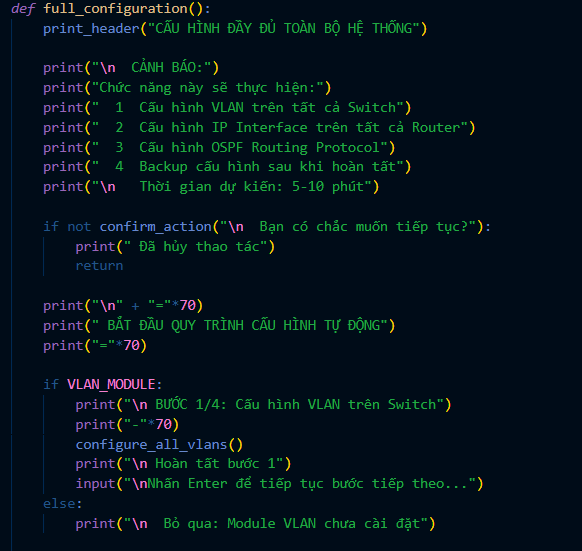
\includegraphics[width=0.7\textwidth]{image/full_cf_1.png}
                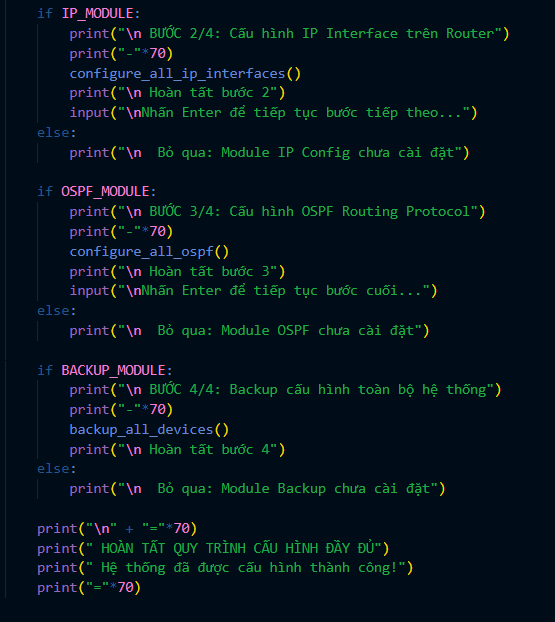
\includegraphics[width=0.7\textwidth]{image/full_cf_2.png}
                \caption{Cấu hình toàn bộ hệ thống}
        \end{figure}
        
        \item system\_info():Hiển thị thông tin hệ thống, modules đã cài đặt.

        \begin{figure}[H]
                \centering
                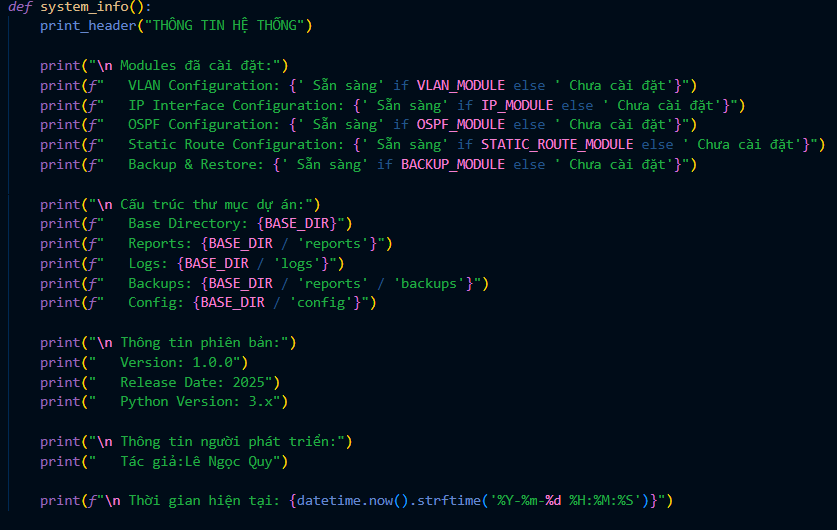
\includegraphics[width=0.7\textwidth]{image/sys_i4.png}
                \caption{Cấu hình hiển thị thông tin hệ thống}
        \end{figure}
        
        \item main\_menu():Menu chính với 4 lựa chọn chính.

        \begin{figure}[H]
                \centering
                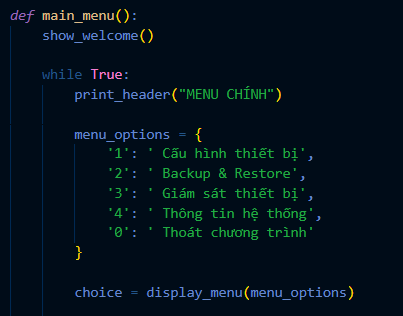
\includegraphics[width=0.7\textwidth]{image/main_menu_1.png}
        \end{figure}

        \begin{figure}[H]
                \centering
                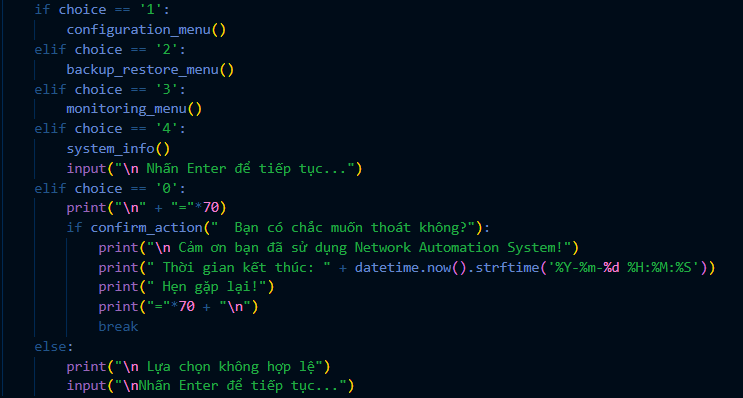
\includegraphics[width=0.7\textwidth]{image/main_menu_2.png}
                \caption{Cấu hình hiển thị thông tin hệ thống}
        \end{figure}

        
        \item main():Hàm khởi chạy chương trình, xử lý ngoại lệ.

        \begin{figure}[H]
                \centering
                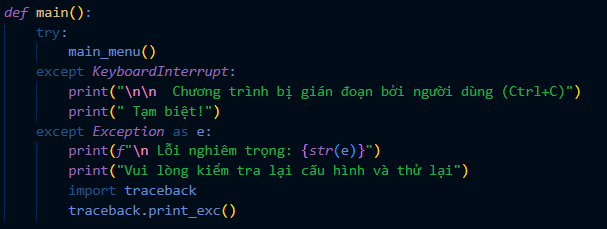
\includegraphics[width=0.7\textwidth]{image/main.png}
                \caption{Cấu hình hiển thị thông tin hệ thống}
        \end{figure}
        
    \end{itemize}

\subsection{Quy trình cấu hình đầy đủ}
\subsubsection{Phần 1: Cấu hình VLAN (vlan_config.py)}
        \begin{itemize}
            \item Đọc danh sách thiết bị và lọc Switch.
            \begin{figure}[H]
                \centering
                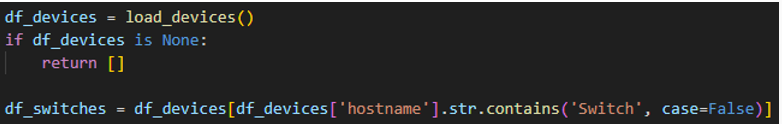
\includegraphics[width=0.7\textwidth]{image/1.png}
            \end{figure}
            Kết quả: Switch1, Switch2, Switch3

            \item Lặp qua từng Switch
            \begin{figure}[H]
                \centering
                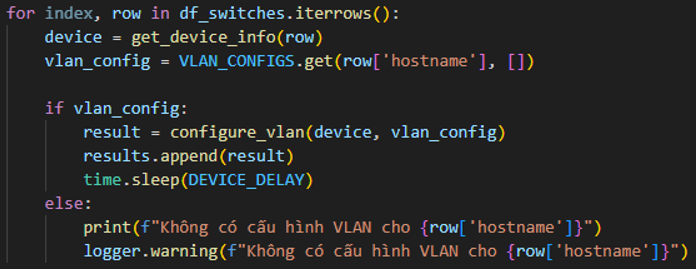
\includegraphics[width=0.7\textwidth]{image/2.png}
            \end{figure}

            \item Kết nối đến Switch
            \begin{figure}[H]
                \centering
                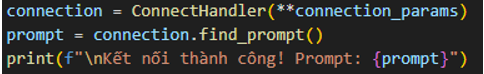
\includegraphics[width=0.7\textwidth]{image/3.png}
            \end{figure}
            \item Gửi lệnh cấu hình VLAN
            \begin{figure}[H]
                \centering
                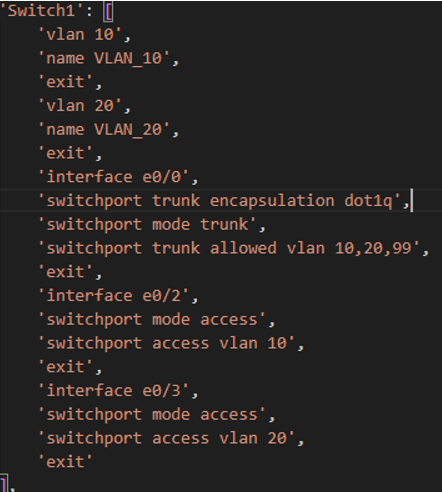
\includegraphics[width=0.7\textwidth]{image/gui_cau_hinh_vlan.png}
            \end{figure}

            \begin{figure}[H]
                \centering
                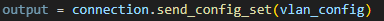
\includegraphics[width=0.7\textwidth]{image/4.png}
            \end{figure}

            \item Lưu cấu hình\\
            connection.save\_config()\\
            Thực hiện: write memory hoặc copy run start
            \item Kiểm tra kết quả \\
            verify\_output = connection.send\_command('show vlan brief')
            \item  Ngắt kết nối\\
            connection.disconnect()
            \item Lưu kết quả \\
            \begin{figure}[H]
                \centering
                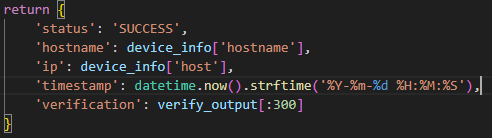
\includegraphics[width=0.7\textwidth]{image/5.png}
            \end{figure}
            \item Lặp lại cho Switch2, Switch3 \\
            time.sleep(DEVICE\_DELAY)  \\
            Tiếp tục với Switch2, Switch3
            \item Xuất báo cáo \\
            output\_file = save\_results(results, 'vlan\_config\_results', REPORTS\_DIR)\\
            File: reports/vlan\_config\_results\_20250122\_103055.csv\\
            Nội dung CSV:
            \begin{figure}[H]
                \centering
                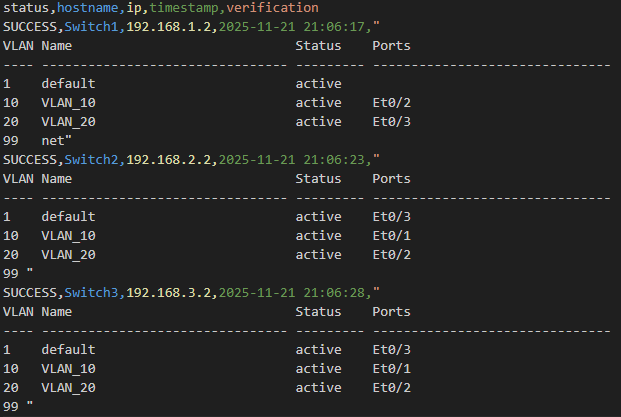
\includegraphics[width=0.7\textwidth]{image/6.png}
            \end{figure}
        \end{itemize}
\subsubsection{Phần 2: Cấu hình IP interface (ip/_config.py)}
        \begin{itemize}
            \item Đọc danh sách thiết bị và lọc Router
            \begin{figure}[H]
                \centering
                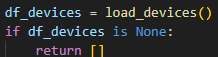
\includegraphics[width=0.7\textwidth]{image/7.png}
            \end{figure}
            Không lọc, lấy tất cả thiết bị (R1, R2, R3 có IP\_CONFIGS)
            \item Kết nối đến R1
            \begin{figure}[H]
                \centering
                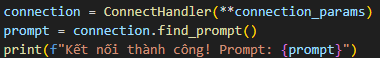
\includegraphics[width=0.7\textwidth]{image/8.png}
            \end{figure}
            \item Gửi lệnh cấu hình IP
            \begin{figure}[H]
                \centering
                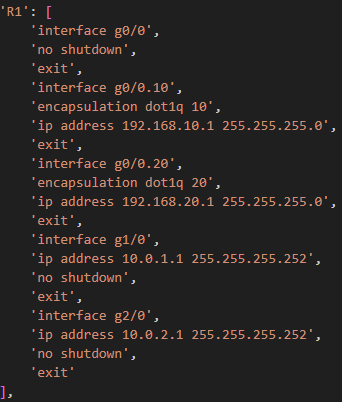
\includegraphics[width=0.7\textwidth]{image/9.png}
            \end{figure}
            \begin{figure}[H]
                \centering
                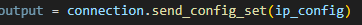
\includegraphics[width=0.7\textwidth]{image/10.png}
            \end{figure}
            \item Lưu và verify
            \begin{figure}[H]
                \centering
                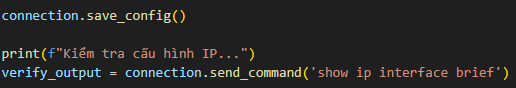
\includegraphics[width=0.7\textwidth]{image/11.png}
            \end{figure}
            Output:
            \begin{figure}[H]
                \centering
                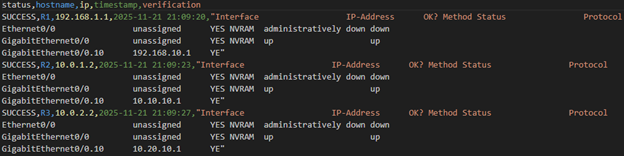
\includegraphics[width=0.7\textwidth]{image/12.png}
            \end{figure}
            \item Lặp lại cho R2, R3
        \end{itemize}    
\subsubsection{Phần 3: Cấu hình OSPF (ospf_config.py)}
        \begin{itemize}
            \item Đọc danh sách thiết bị và lọc Router
            \begin{figure}[H]
                \centering
                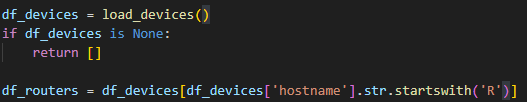
\includegraphics[width=0.7\textwidth]{image/13.png}
            \end{figure}
             Kết quả: R1, R2, R3
             \item Cấu hình OSPF cho R1
             \begin{figure}[H]
                \centering
                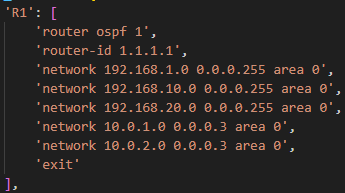
\includegraphics[width=0.7\textwidth]{image/14.png}
            \end{figure}
            \begin{figure}[H]
                \centering
                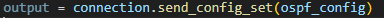
\includegraphics[width=0.7\textwidth]{image/15.png}
            \end{figure}
            \item Chờ OSPF neighbor thiết lập
            \begin{figure}[H]
                \centering
                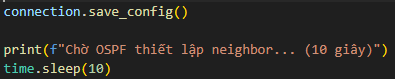
\includegraphics[width=0.7\textwidth]{image/16.png}
            \end{figure}
            \item Verify OSPF
            \begin{figure}[H]
                \centering
                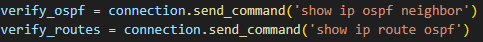
\includegraphics[width=0.7\textwidth]{image/17.png}
            \end{figure}
            Output:
            \begin{figure}[H]
                \centering
                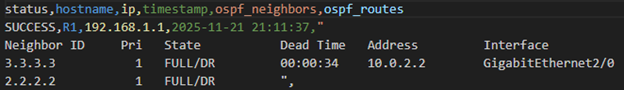
\includegraphics[width=0.7\textwidth]{image/18.png}
            \end{figure}
             Lặp lại cho R2, R3
        \end{itemize}    
\subsubsection{Phần 4: Backup cấu hình (backup_restore.py)} 
        \begin{itemize}
            \item Backup tất cả thiết bị
            \begin{figure}[H]
                \centering
                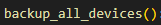
\includegraphics[width=0.7\textwidth]{image/19.png}
            \end{figure}
            \item Lặp qua từng thiết bị
            \begin{figure}[H]
                \centering
                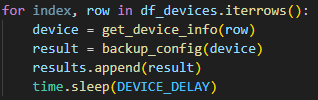
\includegraphics[width=0.7\textwidth]{image/20.png}
            \end{figure}
            \item Kết nối và lấy running-config
            \begin{figure}[H]
                \centering
                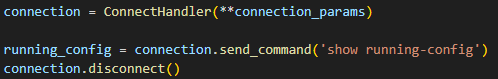
\includegraphics[width=0.7\textwidth]{image/21.png}
            \end{figure}
            Nội dung running\_config:
            \begin{figure}[H]
                \centering
                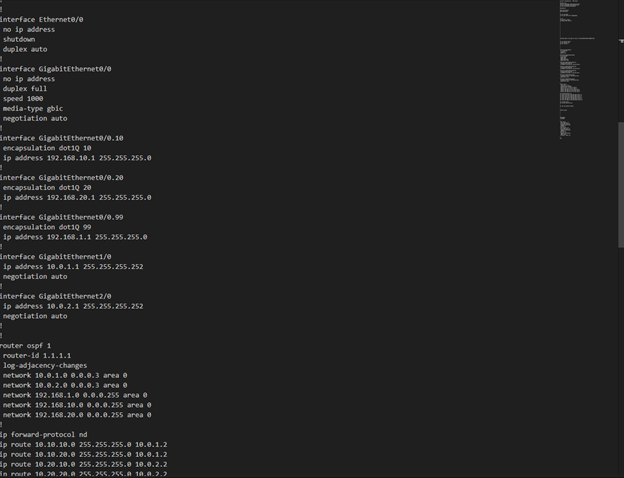
\includegraphics[width=0.7\textwidth]{image/22.png}
            \end{figure}
            \item Lưu vào file
            \begin{figure}[H]
                \centering
                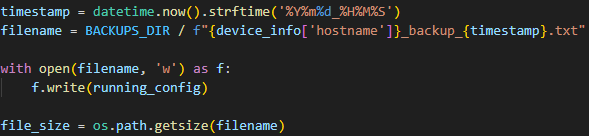
\includegraphics[width=0.7\textwidth]{image/23.png}
            \end{figure}
            \item Kết quả backup
            \begin{figure}[H]
                \centering
                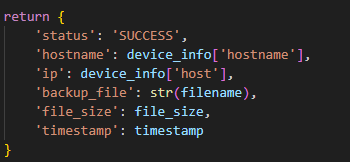
\includegraphics[width=0.7\textwidth]{image/24.png}
            \end{figure}
            \item Lặp lại cho tất cả thiết bị
            Kết quả:
            \begin{verbatim}
                R1_backup_20251122_104500.txt
                R2_backup_20251122_104505.txt
                R3_backup_20251122_104510.txt
                Switch1_backup_20251122_104515.txt
                Switch2_backup_20251122_104520.txt
                Switch3_backup_20251122_104525.txt
            \end{verbatim}
            \item  Xuất báo cáo backup
            \begin{figure}[H]
                \centering
                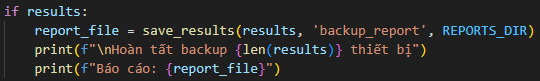
\includegraphics[width=0.7\textwidth]{image/25.png}
            \end{figure}
        \end{itemize}
\subsubsection{Phần 3: Quy trình giám sát (monitoring.py)}    
CHỨC NĂNG 1: Kiểm tra kết nối (check\_device\_connectivity)
    \begin{itemize}
        \item Lặp qua từng thiết bị
        \begin{figure}[H]
            \centering
            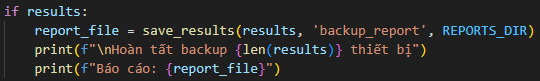
\includegraphics[width=0.7\textwidth]{image/26.png}
        \end{figure}
        \item Kết nối và đo thời gian
        \begin{figure}[H]
            \centering
            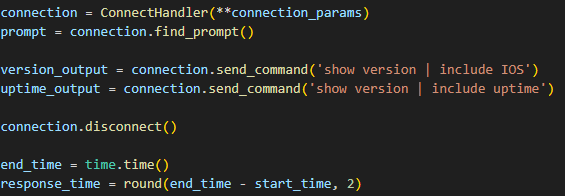
\includegraphics[width=0.7\textwidth]{image/27.png}
        \end{figure}
        \item  Lưu kết quả
        \begin{figure}[H]
            \centering
            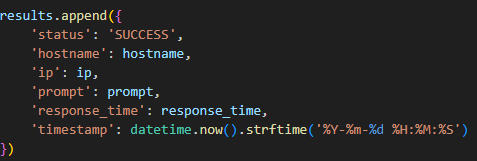
\includegraphics[width=0.7\textwidth]{image/28.png}
        \end{figure}
    \end{itemize}
CHỨC NĂNG 2: Xem trạng thái Interface (show\_interface\_status)       
    \begin{itemize}
        \item Với Switch
        \begin{figure}[H]
            \centering
            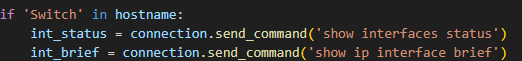
\includegraphics[width=0.7\textwidth]{image/29.png}
        \end{figure}
        \item  Với Router
        \begin{figure}[H]
            \centering
            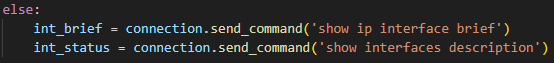
\includegraphics[width=0.7\textwidth]{image/30.png}
        \end{figure}
        \item Thống kê
        \begin{figure}[H]
            \centering
            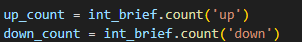
\includegraphics[width=0.7\textwidth]{image/31.png}
        \end{figure}
    \end{itemize}
CHỨC NĂNG 3: Xem bảng định tuyến (show\_routing\_table)
    \begin{itemize}
        \item Chỉ áp dụng cho Router
        \begin{figure}[H]
            \centering
            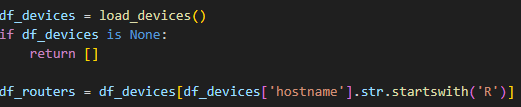
\includegraphics[width=0.7\textwidth]{image/32.png}
        \end{figure}
        \item  Lấy routing table
        \begin{figure}[H]
            \centering
            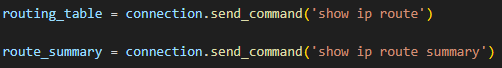
\includegraphics[width=0.7\textwidth]{image/33.png}
        \end{figure}
    \end{itemize}
CHỨC NĂNG 4: Xem VLAN (show\_vlan\_info)
    \begin{itemize}
        \item Chỉ áp dụng cho Switch
         \begin{figure}[H]
            \centering
            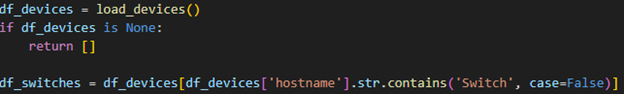
\includegraphics[width=0.7\textwidth]{image/34.png}
        \end{figure}
        \item Lấy thông tin VLAN
        \begin{figure}[H]
            \centering
            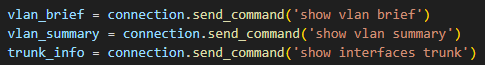
\includegraphics[width=0.7\textwidth]{image/35.png}
        \end{figure}
    \end{itemize}
CHỨC NĂNG 5: Xem OSPF Status (show\_ospf\_status)
    \begin{itemize}
        \item Lấy thông tin OSPF
        \begin{figure}[H]
            \centering
            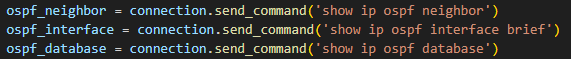
\includegraphics[width=0.7\textwidth]{image/36.png}
        \end{figure}
        \item  Đếm số neighbor 
        \begin{figure}[H]
            \centering
            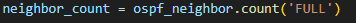
\includegraphics[width=0.7\textwidth]{image/37.png}
        \end{figure}
    \end{itemize}
CHỨC NĂNG 6: Giám sát toàn diện (monitor\_all\_devices)            
    \begin{itemize}
        \item Quy trình:
             \begin{verbatim}
                1.Kiểm tra kết nối → Báo cáo CSV
                2.Kiểm tra Interface → Báo cáo CSV
                3.Kiểm tra Routing Table → Báo cáo CSV
                4.Kiểm tra VLAN → Báo cáo CSV
                5.Kiểm tra OSPF → Báo cáo CSV
                Kết quả: 5 file báo cáo trong thư mục reports/
            \end{verbatim}    
    \end{itemize}
\subsubsection{Phần 4: Quy trình backup/restore}
TÍNH NĂNG 1: Restore từ file backup
    \begin{itemize}
        \item  Chọn thiết bị cần restore
        \begin{figure}[H]
            \centering
            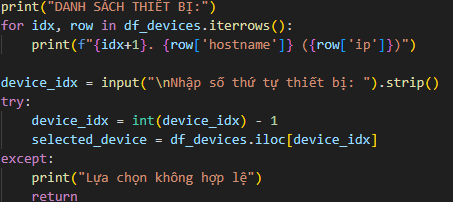
\includegraphics[width=0.7\textwidth]{image/38.png}
        \end{figure}
        \item Hiển thị các file backup
        \begin{figure}[H]
            \centering
            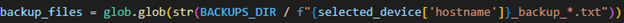
\includegraphics[width=0.7\textwidth]{image/39.png}
        \end{figure}
        \item Chọn file backup
        \begin{figure}[H]
            \centering
            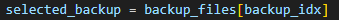
\includegraphics[width=0.7\textwidth]{image/40.png}
        \end{figure}
        \item Xác nhận restore
        \begin{figure}[H]
            \centering
            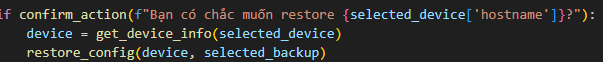
\includegraphics[width=0.7\textwidth]{image/41.png}
        \end{figure}
        \item Đọc file backup
        \begin{figure}[H]
            \centering
            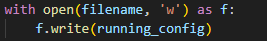
\includegraphics[width=0.7\textwidth]{image/42.png}
        \end{figure}
        \item  Làm sạch cấu hình
        \begin{figure}[H]
            \centering
            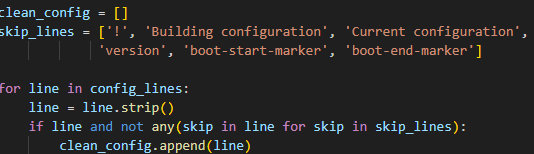
\includegraphics[width=0.7\textwidth]{image/43.png}
        \end{figure}
        \item Áp dụng cấu hình theo batch
        \begin{figure}[H]
            \centering
            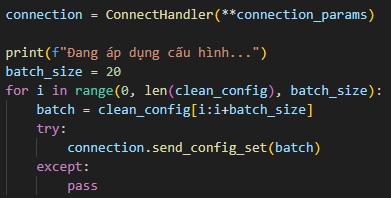
\includegraphics[width=0.7\textwidth]{image/44.png}
        \end{figure}
        \item  Lý do chia batch:
        \begin{verbatim}
            Tránh timeout khi cấu hình quá dài
            Nếu 1 batch lỗi, các batch khác vẫn được áp dụng
            Netmiko có giới hạn số lệnh gửi cùng lúc
        \end{verbatim}
        \item Lưu cấu hình
        \begin{figure}[H]
            \centering
            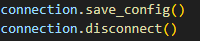
\includegraphics[width=0.7\textwidth]{image/45.png}
        \end{figure}
        \item Kết quả restore
        \begin{figure}[H]
            \centering
            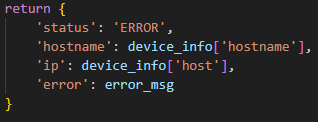
\includegraphics[width=0.7\textwidth]{image/46.png}
        \end{figure}
    \end{itemize}
TÍNH NĂNG 2: Mô phỏng lỗi và tự động khôi phục (simulate\_and\_restore)
    \begin{itemize}
        \item Chọn thiết bị mô phỏng
        \begin{figure}[H]
            \centering
            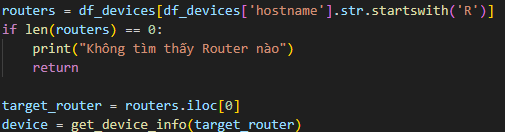
\includegraphics[width=0.7\textwidth]{image/47.png}
        \end{figure}
        \item BƯỚC 1: BACKUP CẤU HÌNH HIỆN TẠI
        \begin{figure}[H]
            \centering
            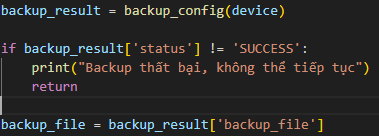
\includegraphics[width=0.7\textwidth]{image/48.png}
        \end{figure}
        \item BƯỚC 2: MÔ PHỎNG LỖI
        \begin{figure}[H]
            \centering
            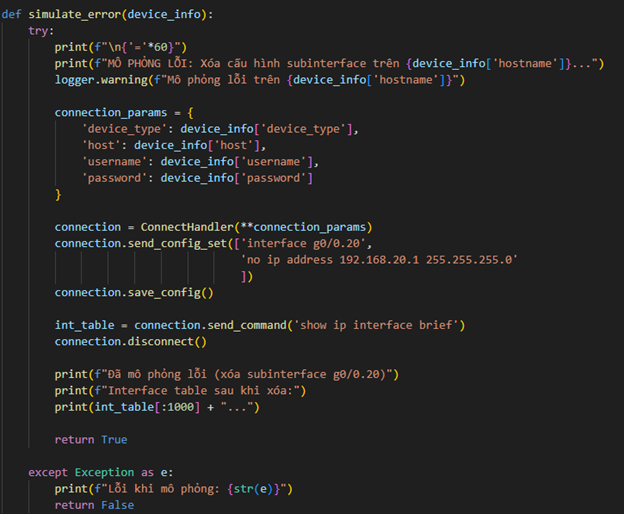
\includegraphics[width=0.7\textwidth]{image/49.png}
        \end{figure}
        \item BƯỚC 3: TỰ ĐỘNG KHÔI PHỤC CẤU HÌNH
        \begin{figure}[H]
            \centering
            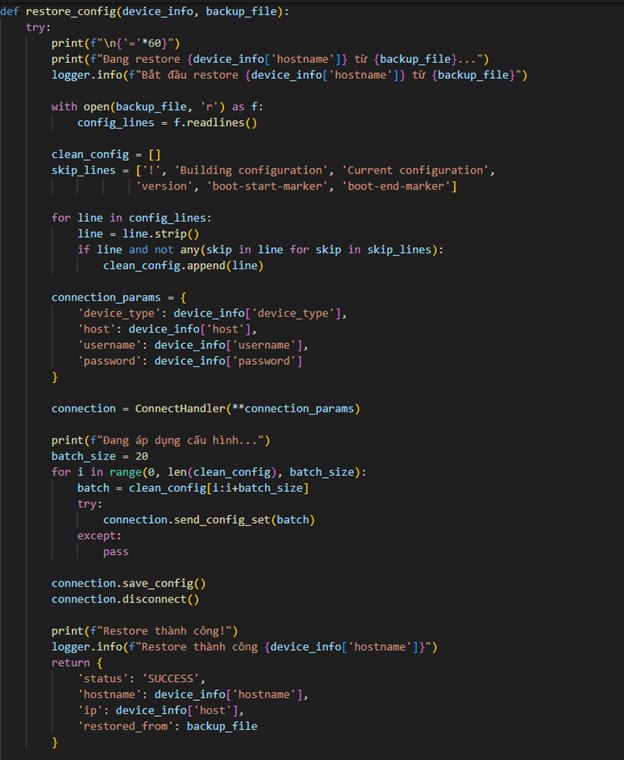
\includegraphics[width=0.7\textwidth]{image/50.png}
        \end{figure}
    \end{itemize}

        




	\newpage \clearpage

	\section*{CHƯƠNG 5 - KẾT QUẢ DEMO}
\addcontentsline{toc}{section}{\numberline{}CHƯƠNG 5 -  KẾT QUẢ DEMO}
\setcounter{section}{5}
\setcounter{subsection}{0}
\setcounter{figure}{0}
\setcounter{table}{0}

%-------------Phần trình bày nội dung chương 5

\subsection{ Tự động cấu hình hóa VLAN:}
\_Kết nối và cấu hình VLAN cho Switch1:

    \begin{figure}[H]
        \centering
        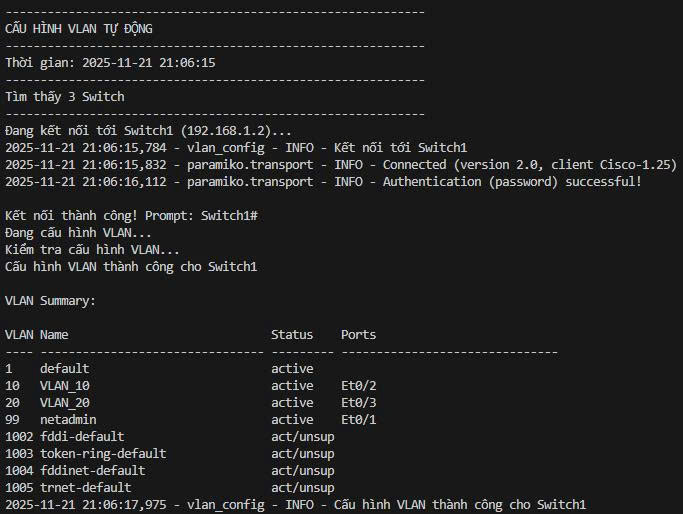
\includegraphics[width=0.7\textwidth]{image/vlan_1.jpg}
        \caption{Cấu hình VLAN cho Switch1}
    \end{figure} % Bắt buộc phải có lệnh này

\_Kết nối và cấu hình VLAN cho Switch2:

     \begin{figure}[H]
        \centering
        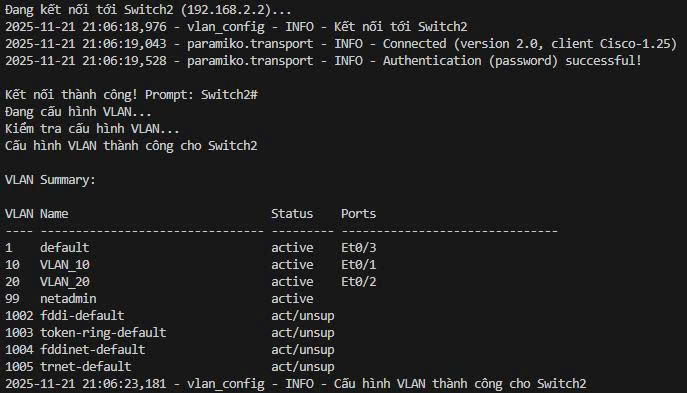
\includegraphics[width=0.7\textwidth]{image/vlan_2.jpg}
        \caption{Cấu hình VLAN cho Switch2}
    \end{figure} % Bắt buộc phải có lệnh này

\_Kết nối và cấu hình VLAN cho Switch3:

    \begin{figure}[H]
        \centering
        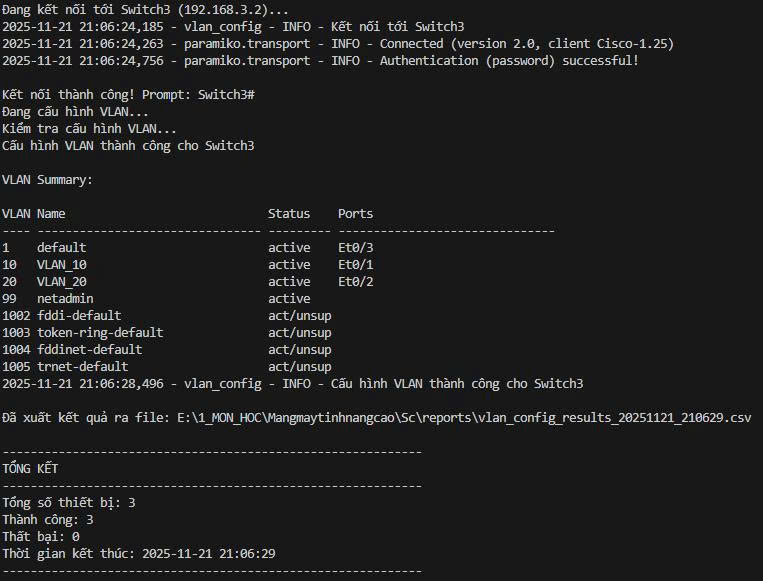
\includegraphics[width=0.7\textwidth]{image/vlan_3.jpg}
        \caption{Cấu hình VLAN cho Switch3}
    \end{figure} % Bắt buộc phải có lệnh này

\subsection{Tự động hóa cấu hình IP:}

\_Kết nối và cấu hình IP cho Router1:

    \begin{figure}[H]
        \centering
        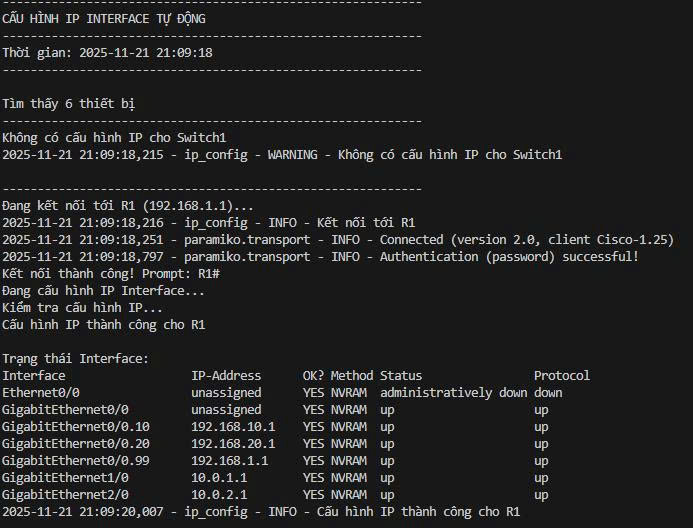
\includegraphics[width=0.7\textwidth]{image/IP_1.jpg}
        \caption{Cấu hình IP cho Router1}
    \end{figure} % Bắt buộc phải có lệnh này

\_Kết nối và cấu hình IP cho Router2:

    \begin{figure}[H]
        \centering
        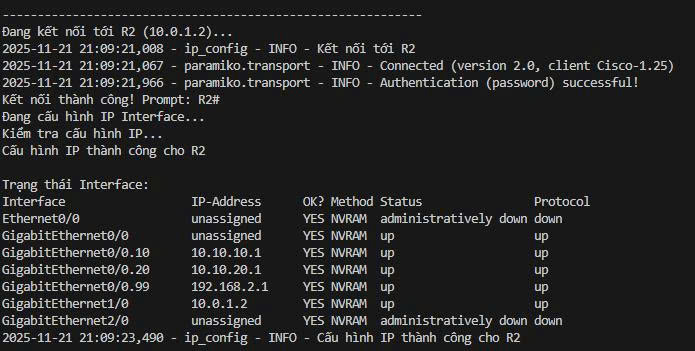
\includegraphics[width=0.7\textwidth]{image/IP_2.jpg}
        \caption{Cấu hình IP cho Router2}
    \end{figure} % Bắt buộc phải có lệnh này

\_Kết nối và cấu hình IP cho Router3:

    \begin{figure}[H]
        \centering
        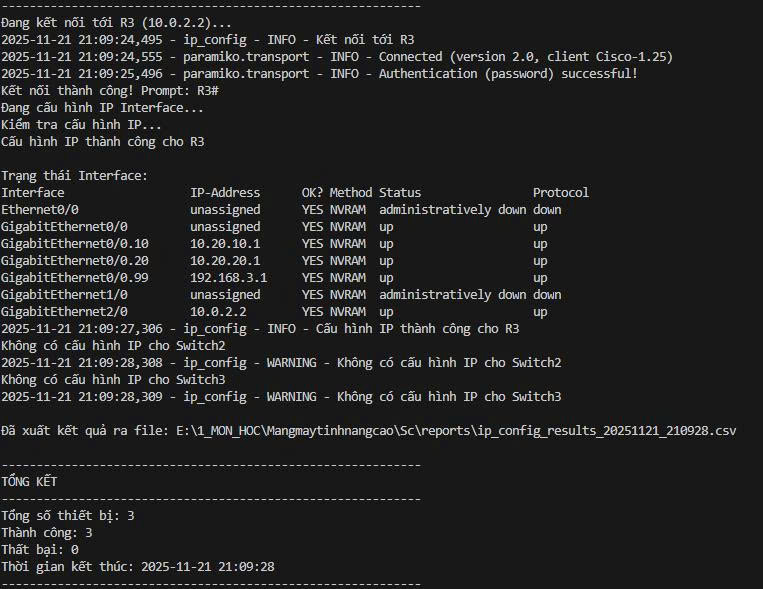
\includegraphics[width=0.7\textwidth]{image/IP_3.jpg}
        \caption{Cấu hình IP cho Router3}
    \end{figure} % Bắt buộc phải có lệnh này

\subsection{Tự động hóa cấu hình OSPF:}

\_Kết nối và cấu hình OSPF cho Router1:

    \begin{figure}[H]
        \centering
        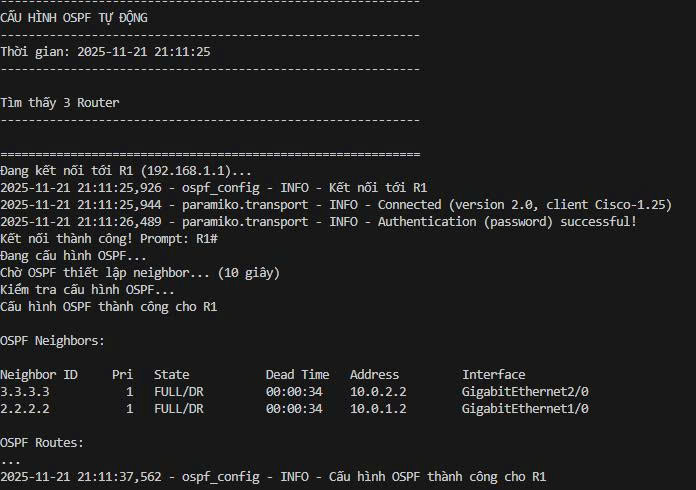
\includegraphics[width=0.7\textwidth]{image/OSPF_1.jpg}
        \caption{Cấu hình OSPF cho Router1}
    \end{figure} % Bắt buộc phải có lệnh này

\_Kết nối và cấu hình OSPF cho Router2:

    \begin{figure}[H]
        \centering
        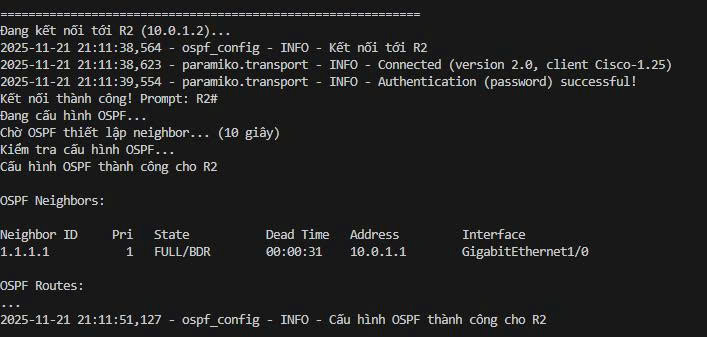
\includegraphics[width=0.7\textwidth]{image/OSPF_2.jpg}
        \caption{Cấu hình OSPF cho Router2}
    \end{figure} % Bắt buộc phải có lệnh này

\_Kết nối và cấu hình OSPF cho Router3:

    \begin{figure}[H]
        \centering
        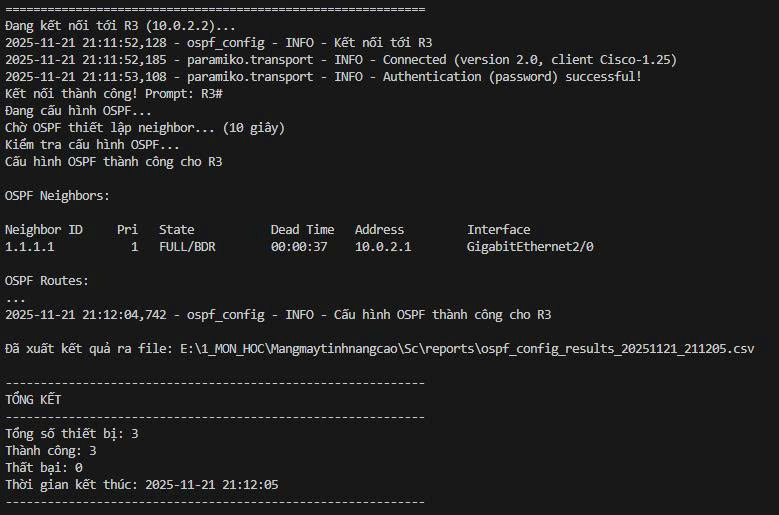
\includegraphics[width=0.7\textwidth]{image/OSPF_3.jpg}
        \caption{Cấu hình OSPF cho Router3}
    \end{figure} % Bắt buộc phải có lệnh này

\subsection{Tự động hóa cấu hình STATIC:}

\_Kết nối và cấu hình STATIC\_ROUTE cho Router1:

    \begin{figure}[H]
        \centering
        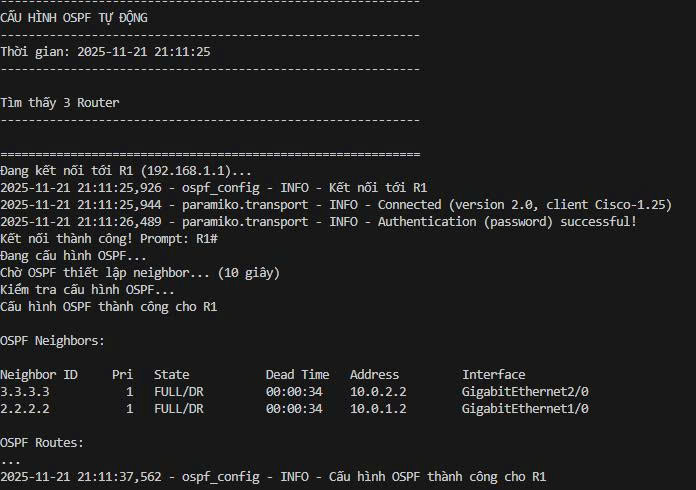
\includegraphics[width=0.7\textwidth]{image/OSPF_1.jpg}
        \caption{Cấu hình STATIC\_ROUTE cho Router1}
    \end{figure} % Bắt buộc phải có lệnh này

\_Kết nối và cấu hình STATIC\_ROUTE cho Router2:

    \begin{figure}[H]
        \centering
        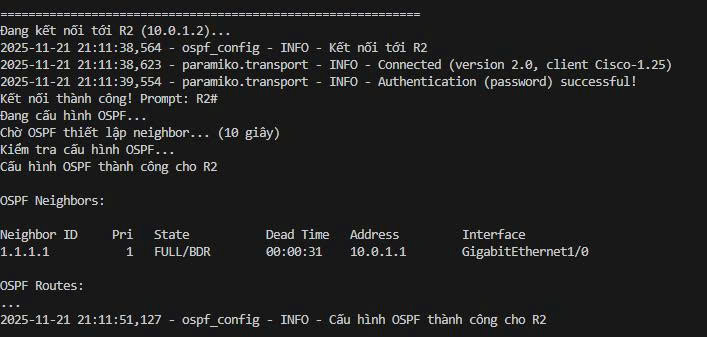
\includegraphics[width=0.7\textwidth]{image/OSPF_2.jpg}
        \caption{Cấu hình STATIC\_ROUTE cho Router2}
    \end{figure} % Bắt buộc phải có lệnh này

\_Kết nối và cấu hình STATIC\_ROUTE cho Router3:

    \begin{figure}[H]
        \centering
        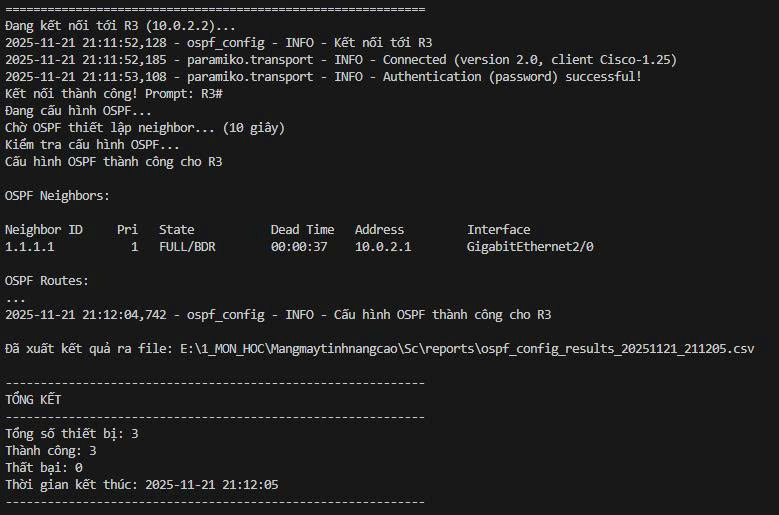
\includegraphics[width=0.7\textwidth]{image/OSPF_3.jpg}
        \caption{Cấu hình STATIC\_ROUTE cho Router3}
    \end{figure} % Bắt buộc phải có lệnh này

\subsection{Cấu hình cho back\_up và restore:}

    \begin{figure}[H]
        \centering
        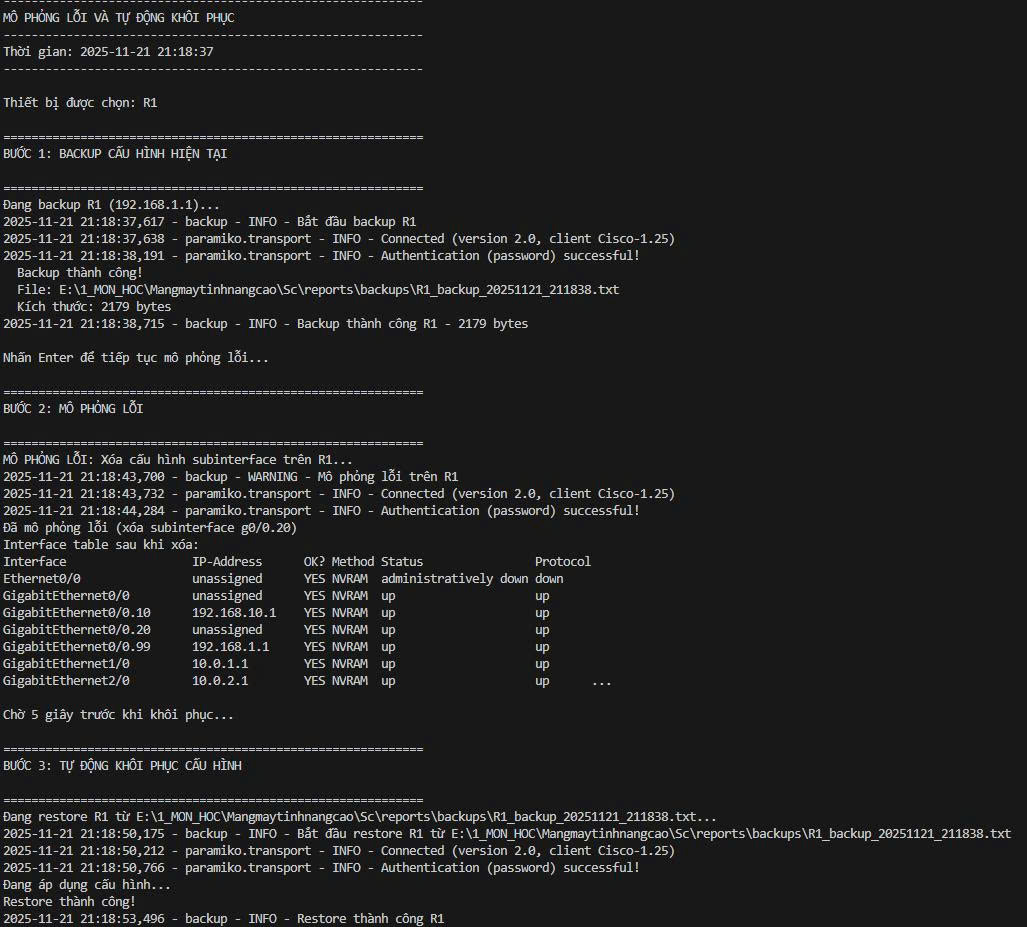
\includegraphics[width=0.7\textwidth]{image/back_up&rstore.jpg}
        \caption{Cấu hình back\_up\&restore}
    \end{figure} % Bắt buộc phải có lệnh này

\subsection{Tự động cấu hình giám sát:}
\_Kiểm tra kết nối thiết bị:

    \begin{figure}[H]
        \centering
        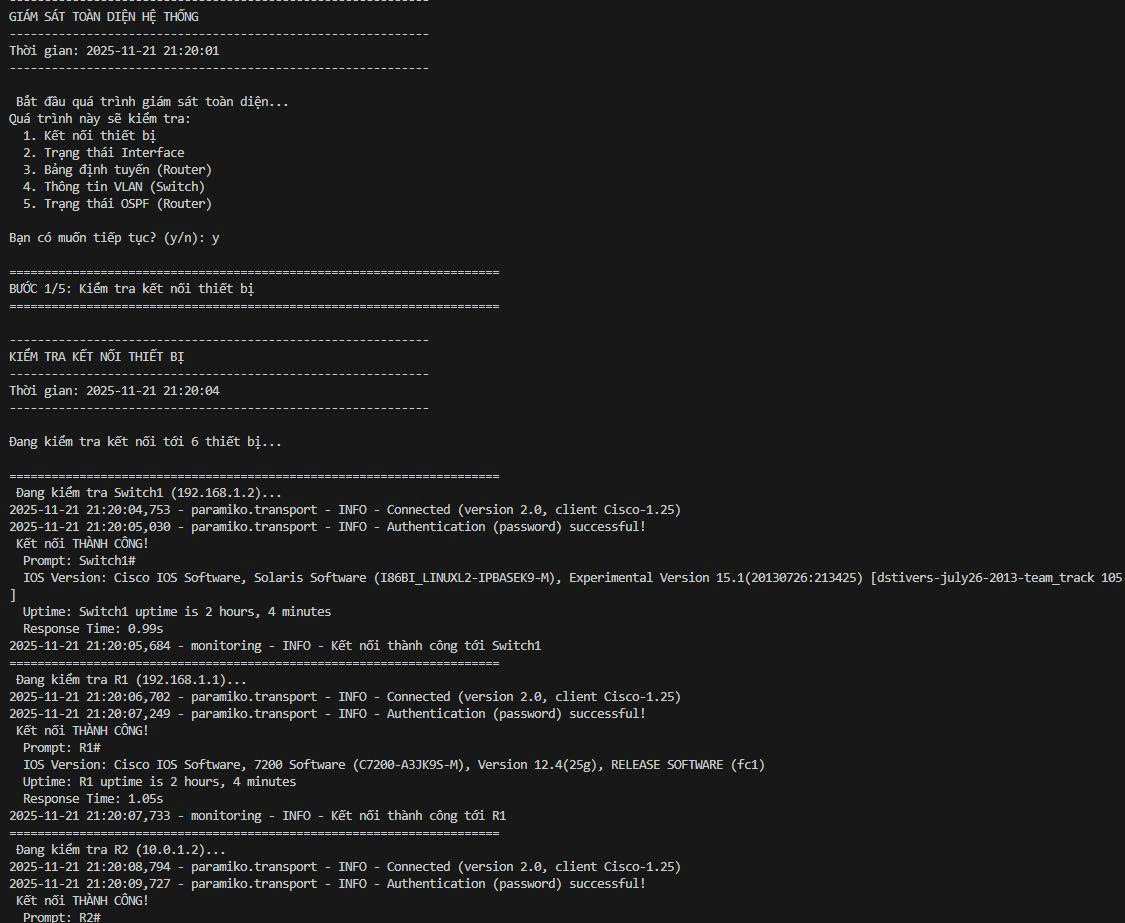
\includegraphics[width=0.7\textwidth]{image/mn_1.jpg}
        \caption{Thực hiện kiểm tra kết nối}
    \end{figure} % Bắt buộc phải có lệnh này

    \begin{figure}[H]
        \centering
        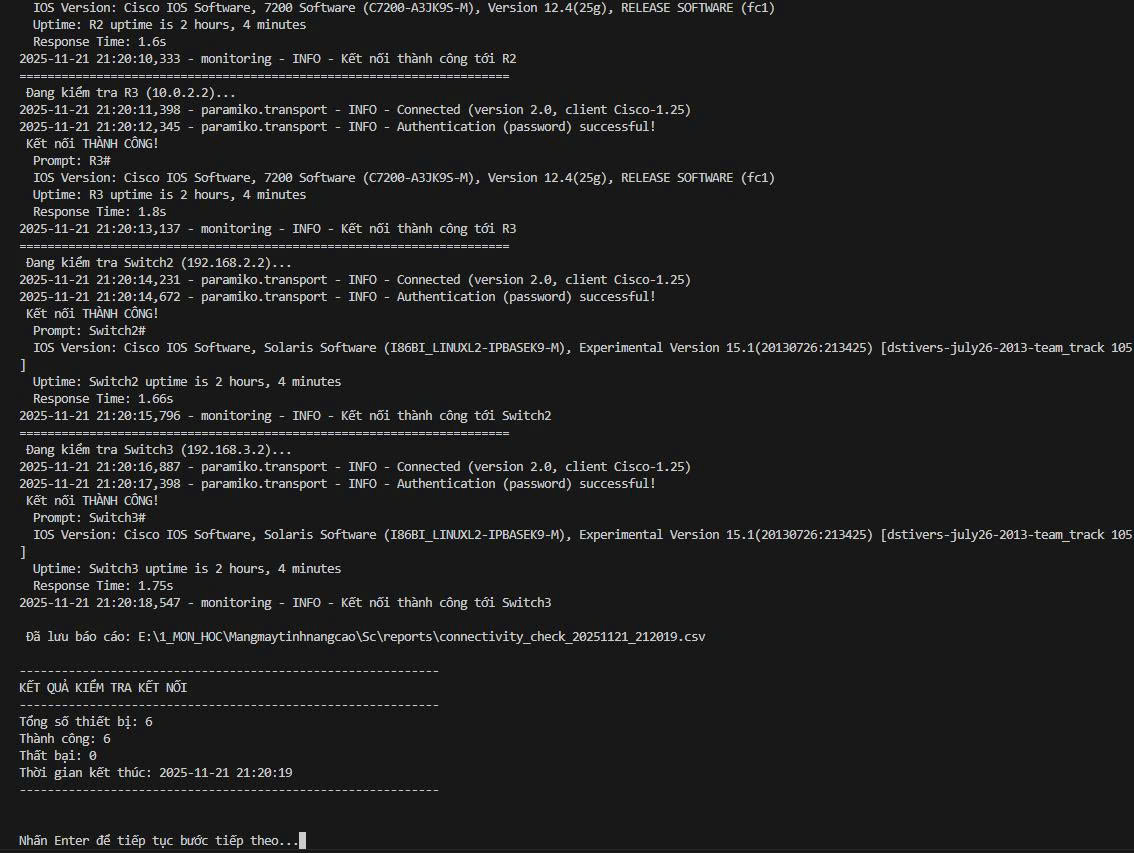
\includegraphics[width=0.7\textwidth]{image/mn_2.jpg}
        \caption{Thực hiện kiểm tra kết nối}
    \end{figure} % Bắt buộc phải có lệnh này

\_Kiểm tra trạng thái interface:

    \begin{figure}[H]
        \centering
        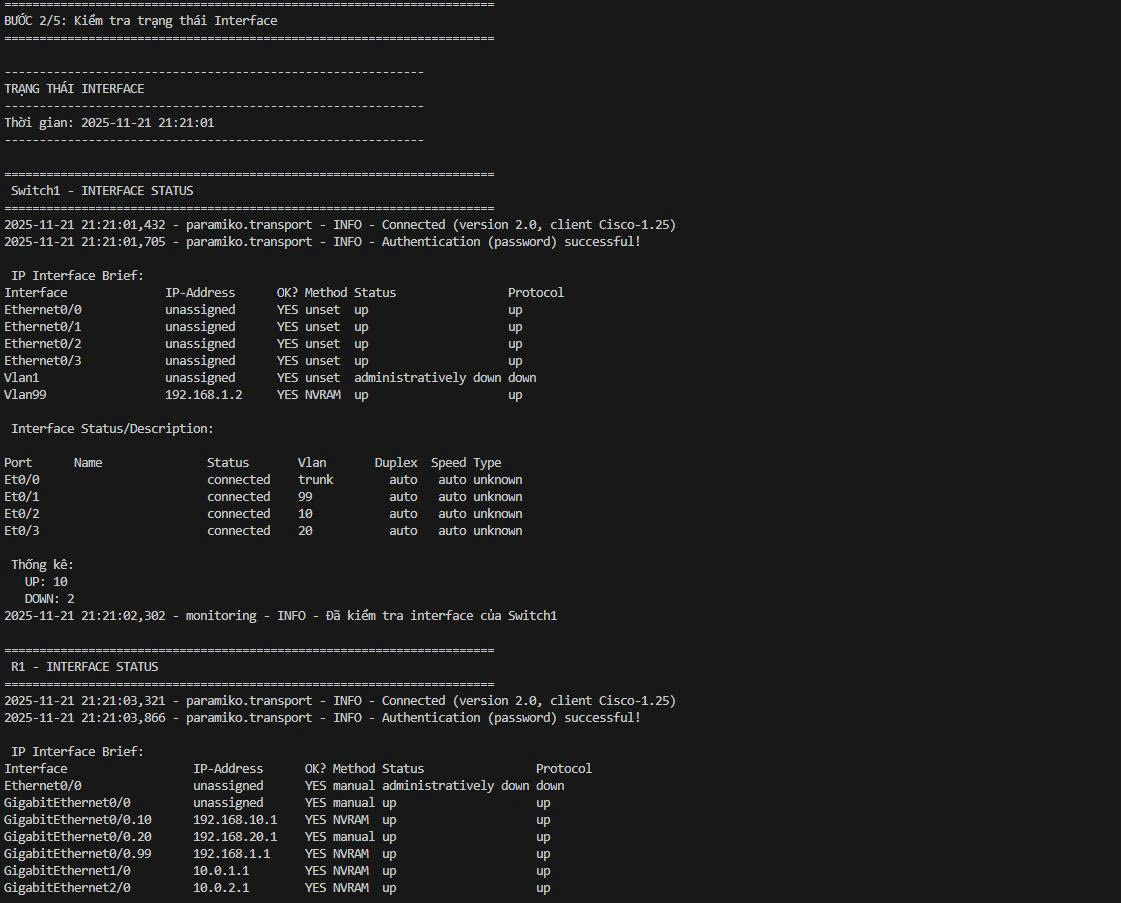
\includegraphics[width=0.7\textwidth]{image/mn_3.jpg}
        \caption{Kiểm tra trạng thái interface}
    \end{figure} % Bắt buộc phải có lệnh này

    \begin{figure}[H]
        \centering
        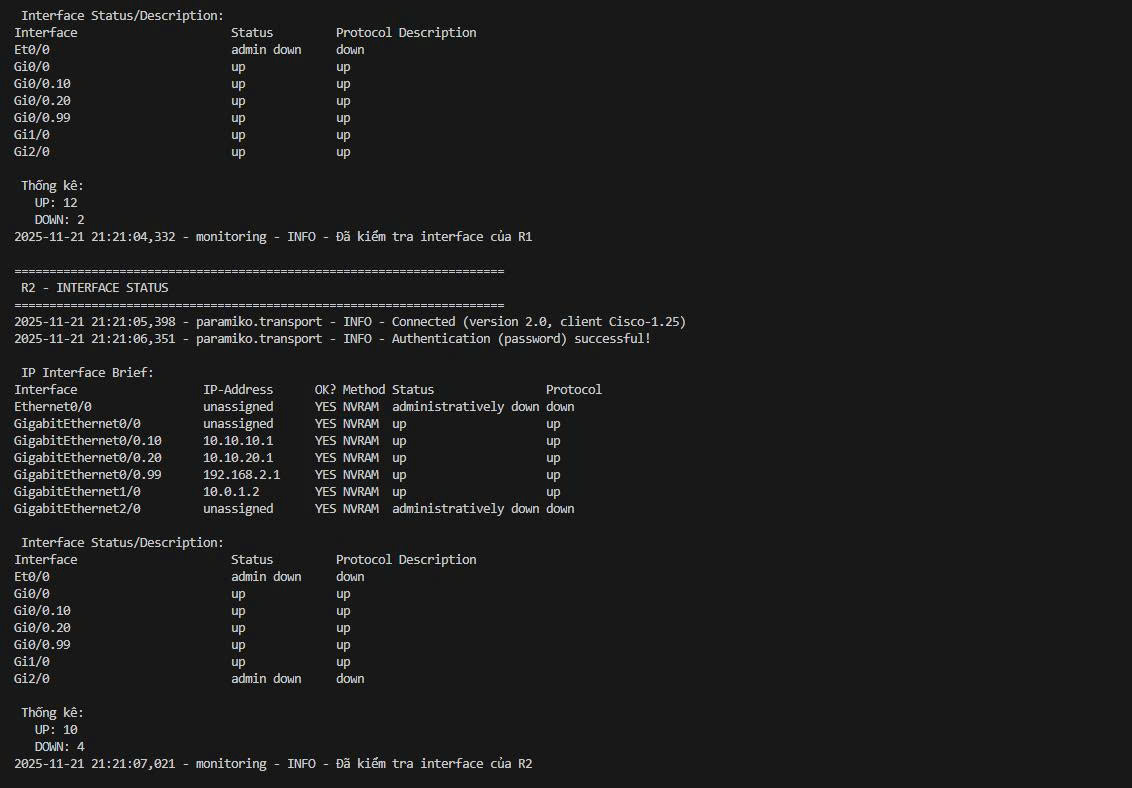
\includegraphics[width=0.7\textwidth]{image/mn_4.jpg}
        \caption{Kiểm tra trạng thái interface}
    \end{figure} % Bắt buộc phải có lệnh này

    \begin{figure}[H]
        \centering
        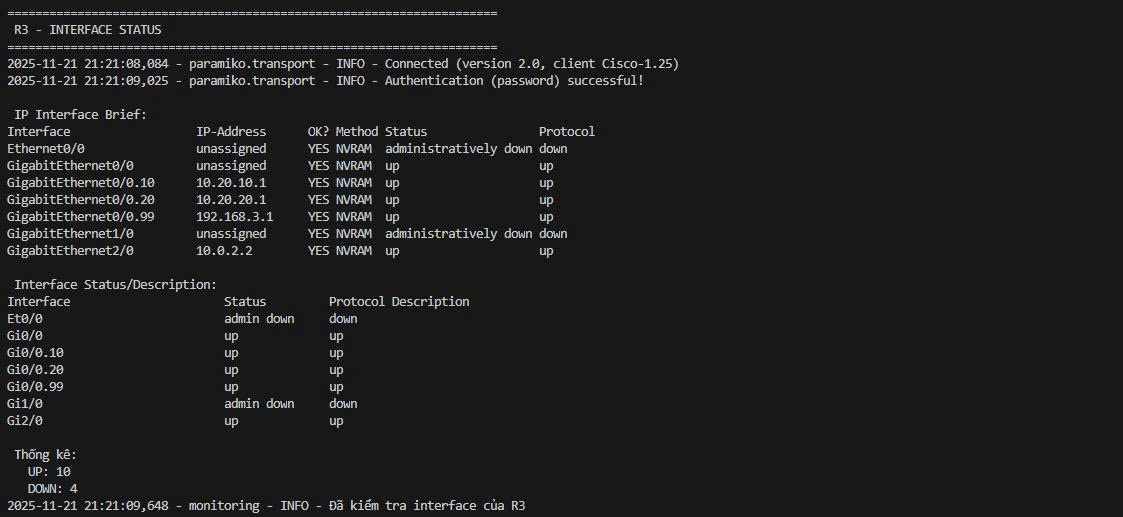
\includegraphics[width=0.7\textwidth]{image/mn_5.jpg}
        \caption{Kiểm tra trạng thái interface}
    \end{figure} % Bắt buộc phải có lệnh này

    
    \begin{figure}[H]
        \centering
        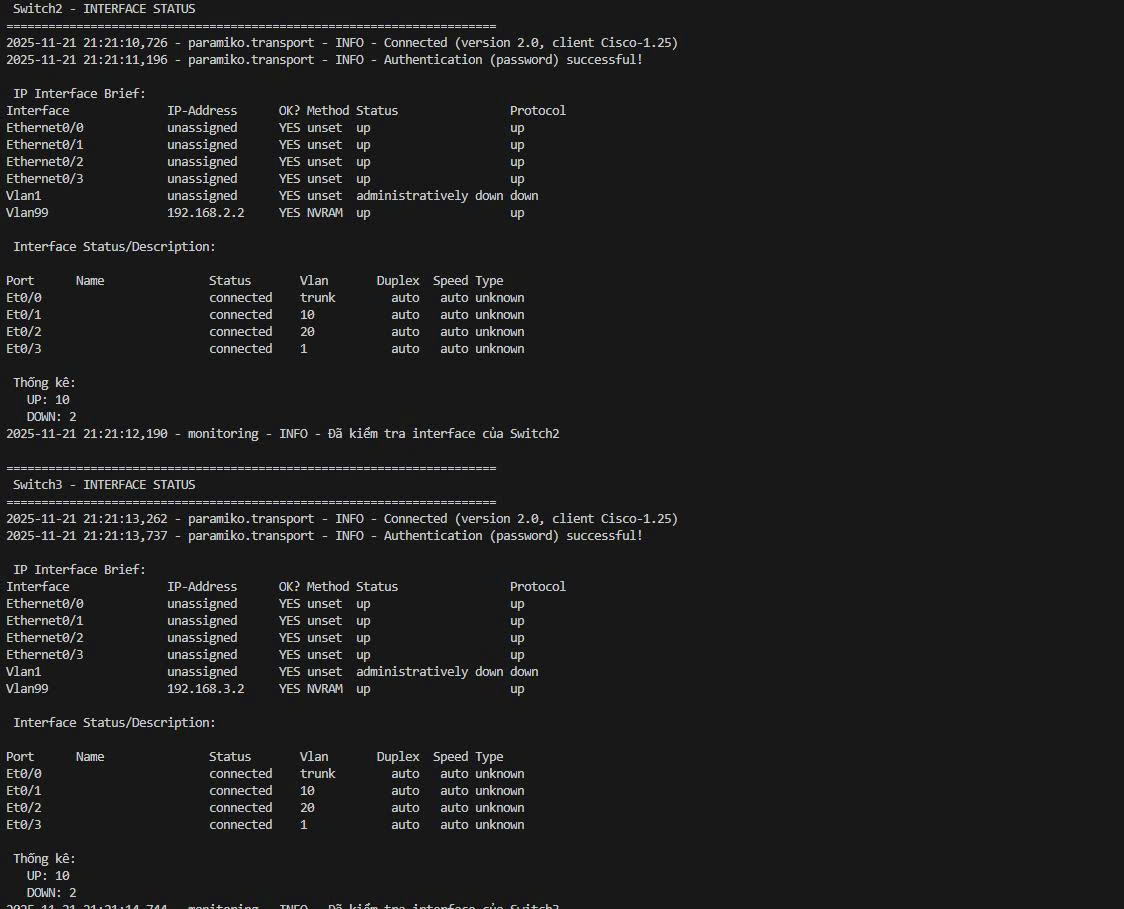
\includegraphics[width=0.7\textwidth]{image/mn_6.jpg}
        \caption{Kiểm tra trạng thái interface}
    \end{figure} % Bắt buộc phải có lệnh này

\_Kiểm tra định tuyến:

    \begin{figure}[H]
        \centering
        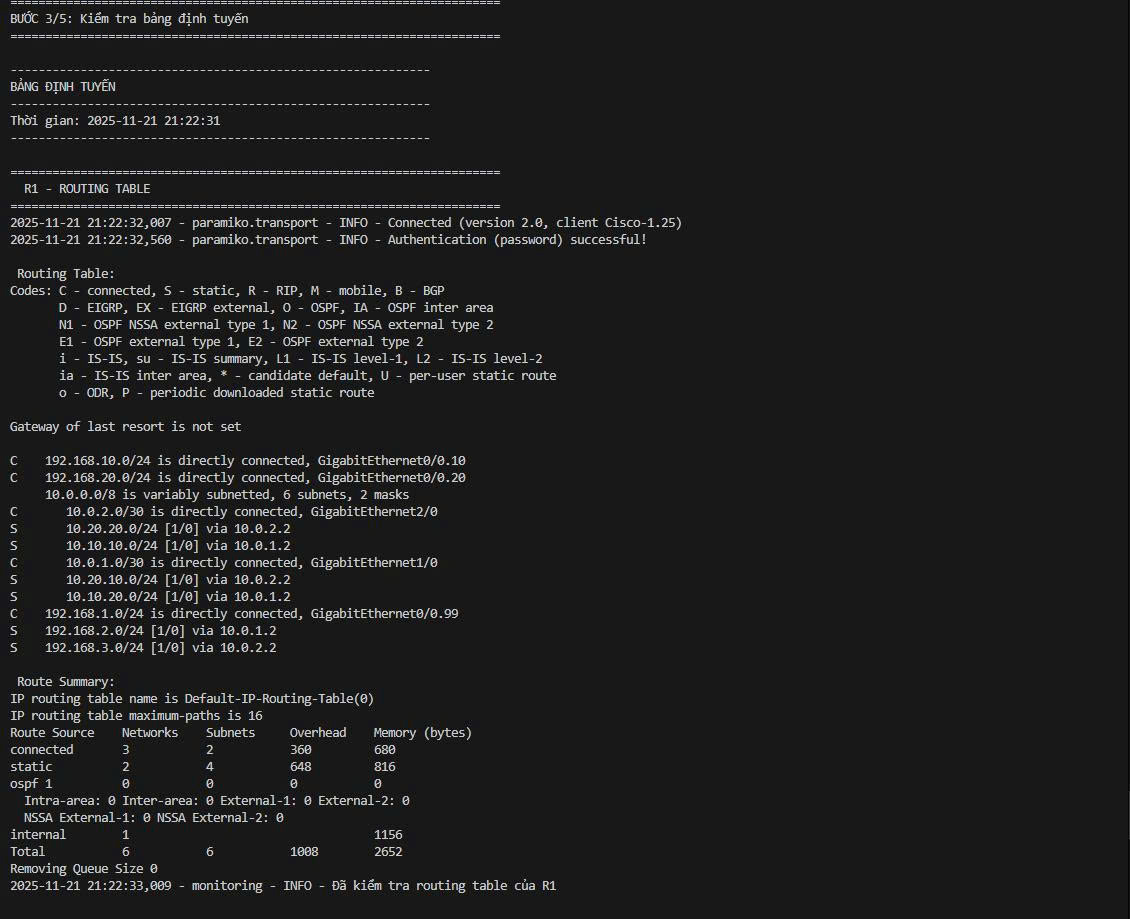
\includegraphics[width=0.7\textwidth]{image/mn_7.jpg}
        \caption{Kiểm tra định tuyến}
    \end{figure} % Bắt buộc phải có lệnh này

    \begin{figure}[H]
        \centering
        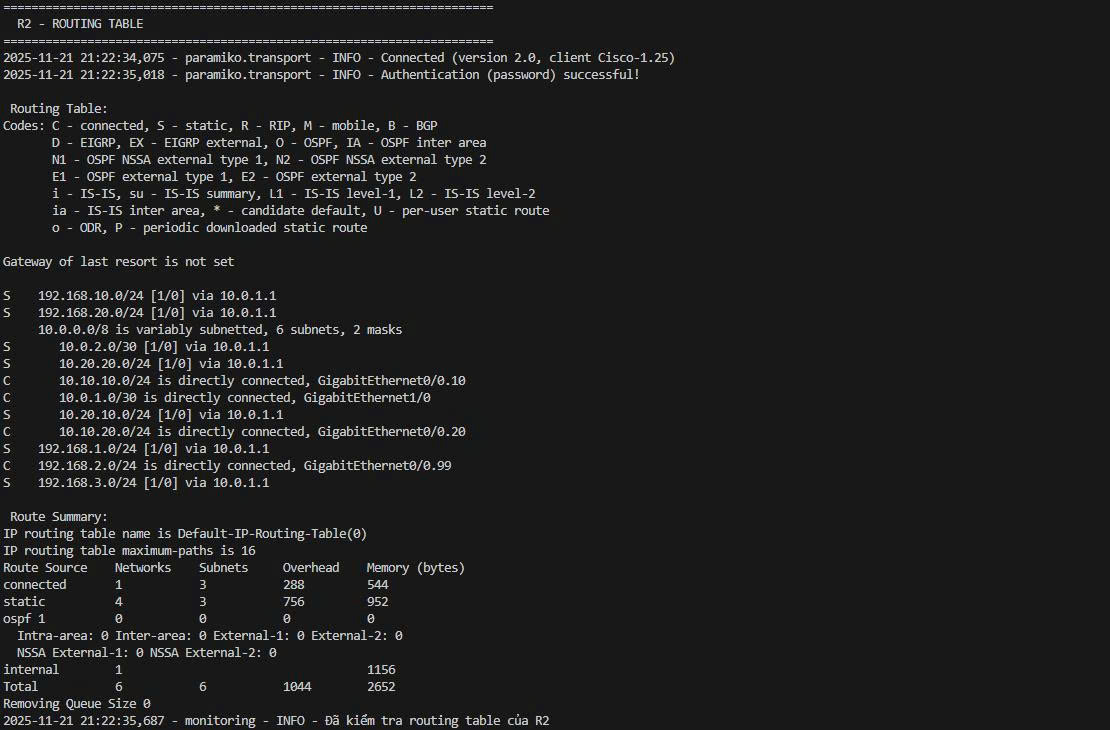
\includegraphics[width=0.7\textwidth]{image/mn_8.jpg}
        \caption{Kiểm tra định tuyến}
    \end{figure} % Bắt buộc phải có lệnh này

    \begin{figure}[H]
        \centering
        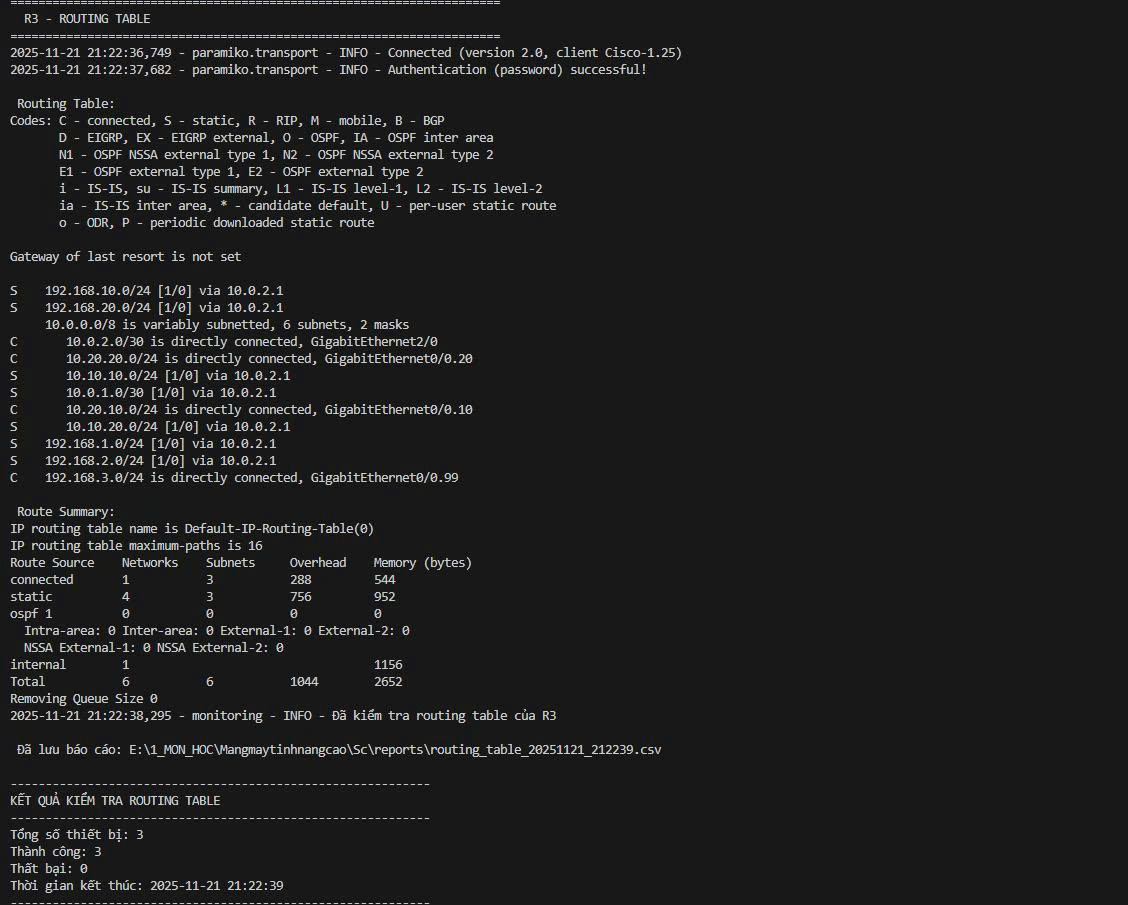
\includegraphics[width=0.7\textwidth]{image/mn_9.jpg}
        \caption{Kiểm tra định tuyến}
    \end{figure} % Bắt buộc phải có lệnh này

\_Kiểm tra cấu hình VLAN:

    \begin{figure}[H]
        \centering
        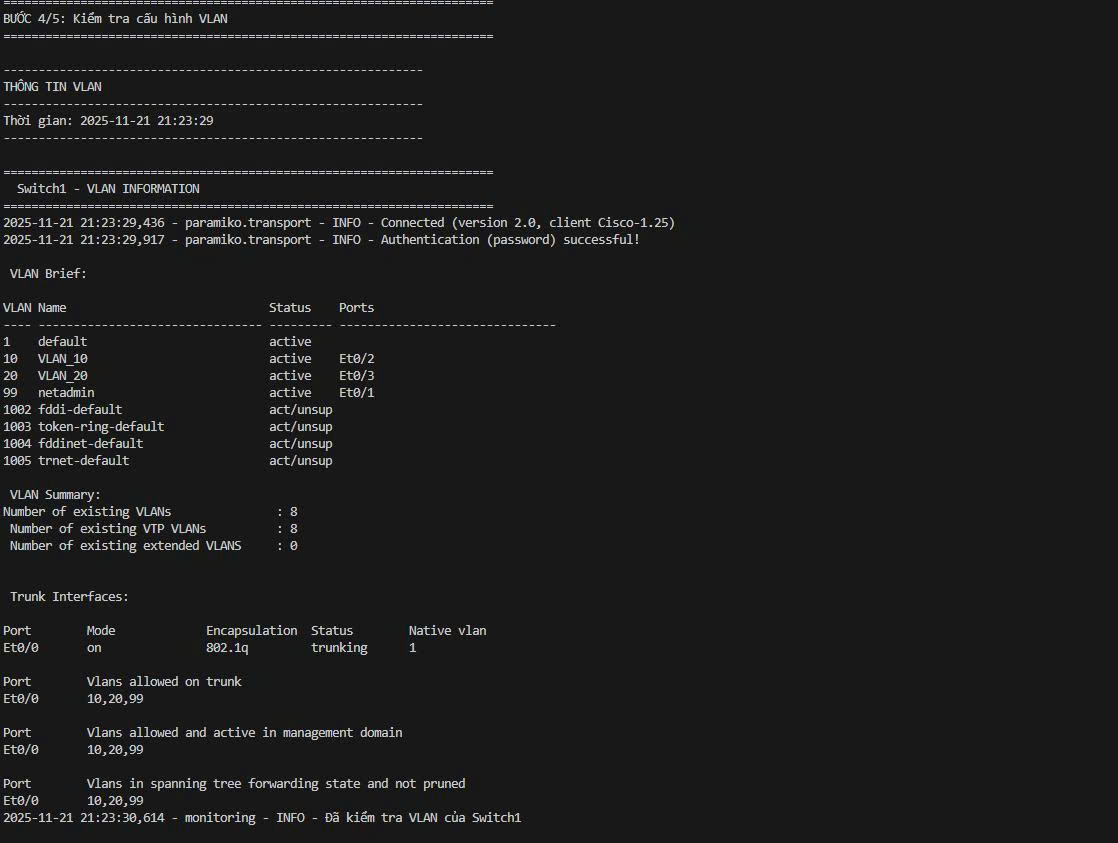
\includegraphics[width=0.7\textwidth]{image/mn_10.jpg}
        \caption{Kiểm tra cấu hình VLAN}
    \end{figure} % Bắt buộc phải có lệnh này

    \begin{figure}[H]
        \centering
        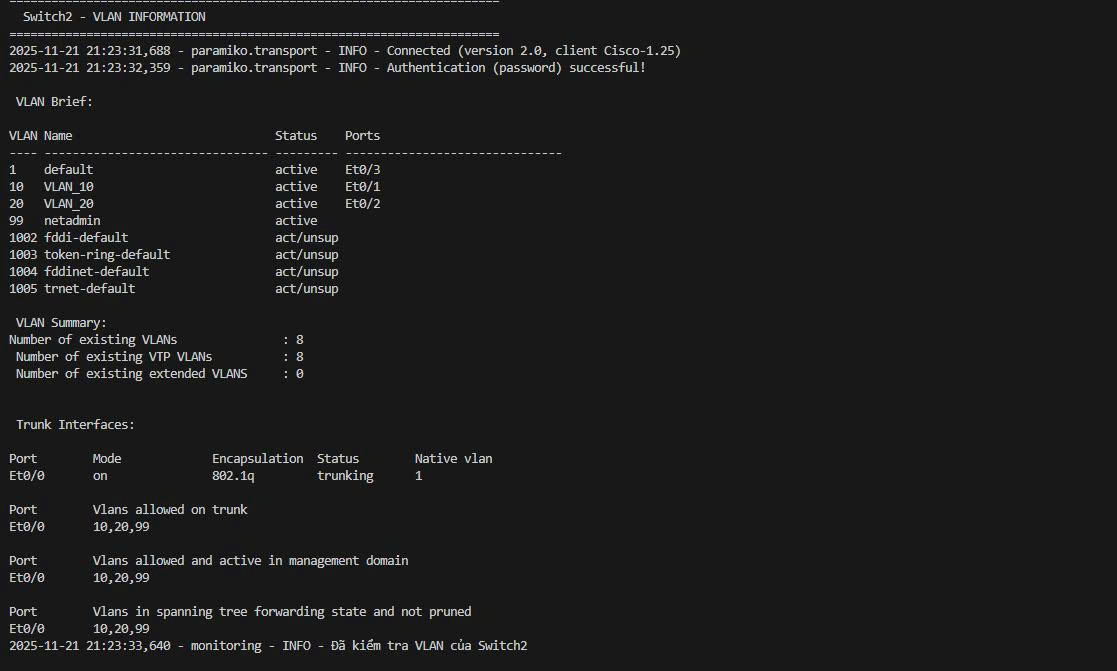
\includegraphics[width=0.7\textwidth]{image/mn_11.jpg}
        \caption{Kiểm tra cấu hình VLAN}
    \end{figure} % Bắt buộc phải có lệnh này

    \begin{figure}[H]
        \centering
        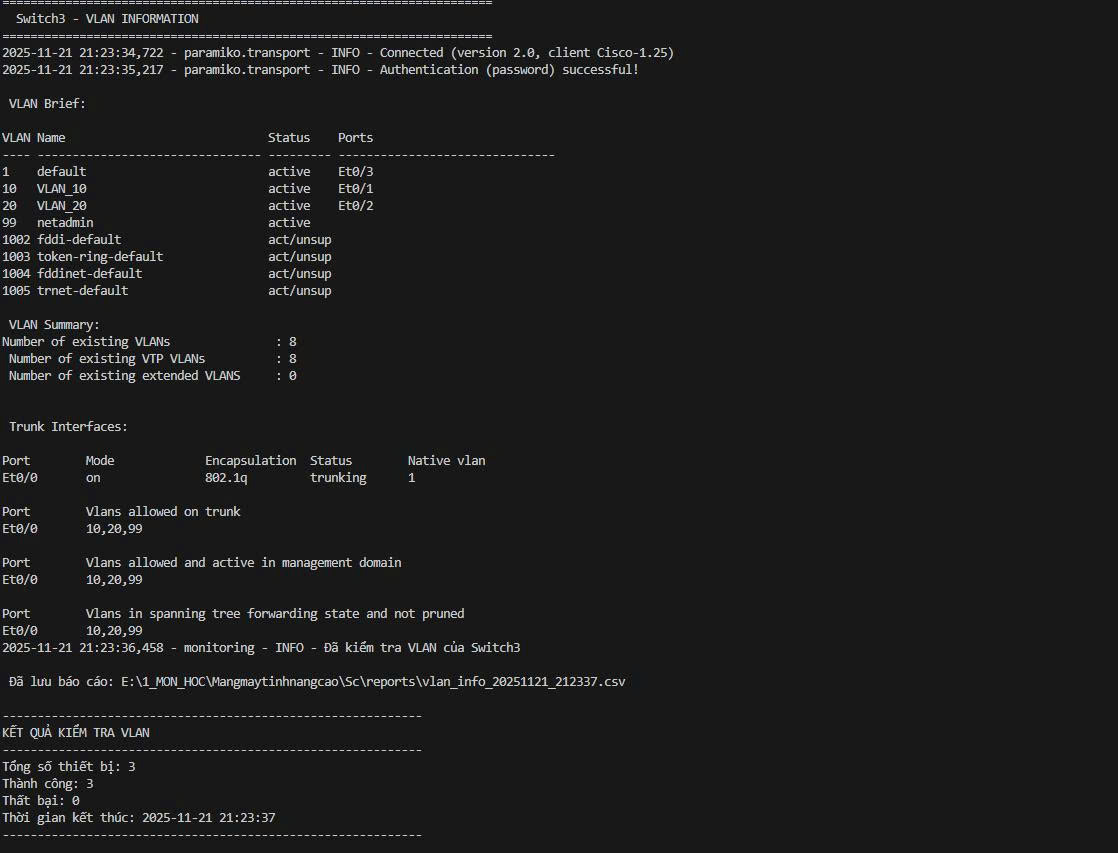
\includegraphics[width=0.7\textwidth]{image/mn_12.jpg}
        \caption{Kiểm tra cấu hình VLAN}
    \end{figure} % Bắt buộc phải có lệnh này

\_Kiểm tra trạng thái OSPF:

    \begin{figure}[H]
        \centering
        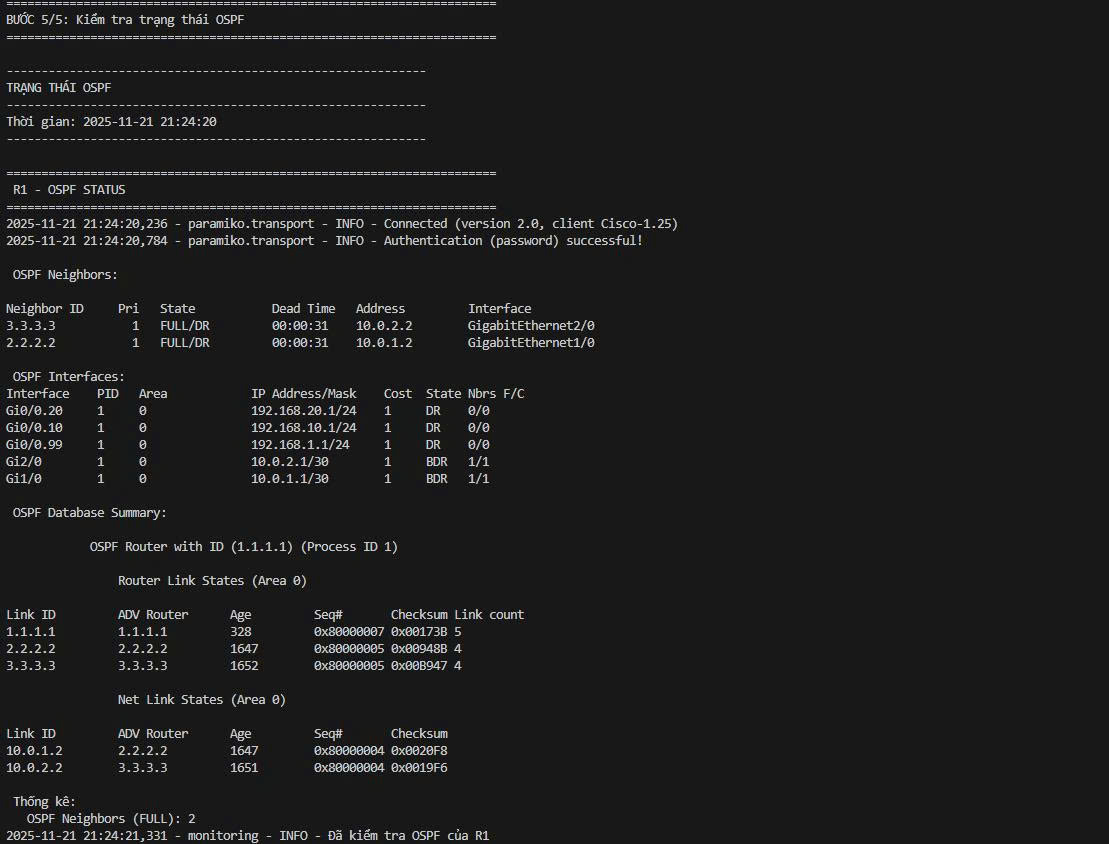
\includegraphics[width=0.7\textwidth]{image/mn_13.jpg}
        \caption{Kiểm tra trạng thái OSPF}
    \end{figure} % Bắt buộc phải có lệnh này

    \begin{figure}[H]
        \centering
        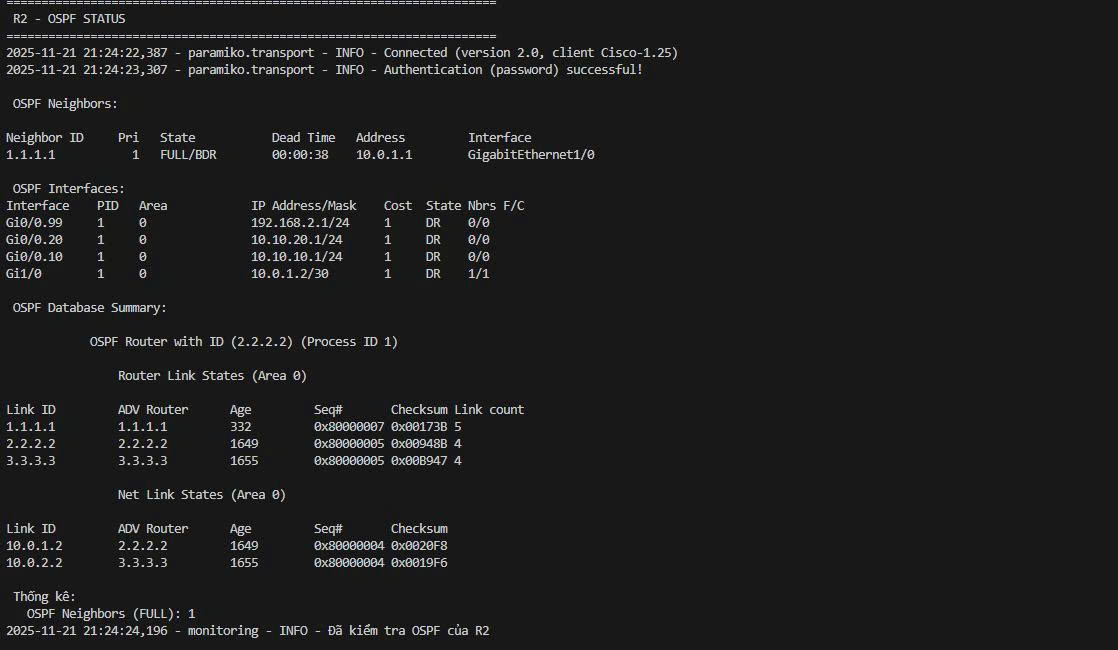
\includegraphics[width=0.7\textwidth]{image/mn_14.jpg}
        \caption{Kiểm tra trạng thái OSPF}
    \end{figure} % Bắt buộc phải có lệnh này

    \begin{figure}[H]
        \centering
        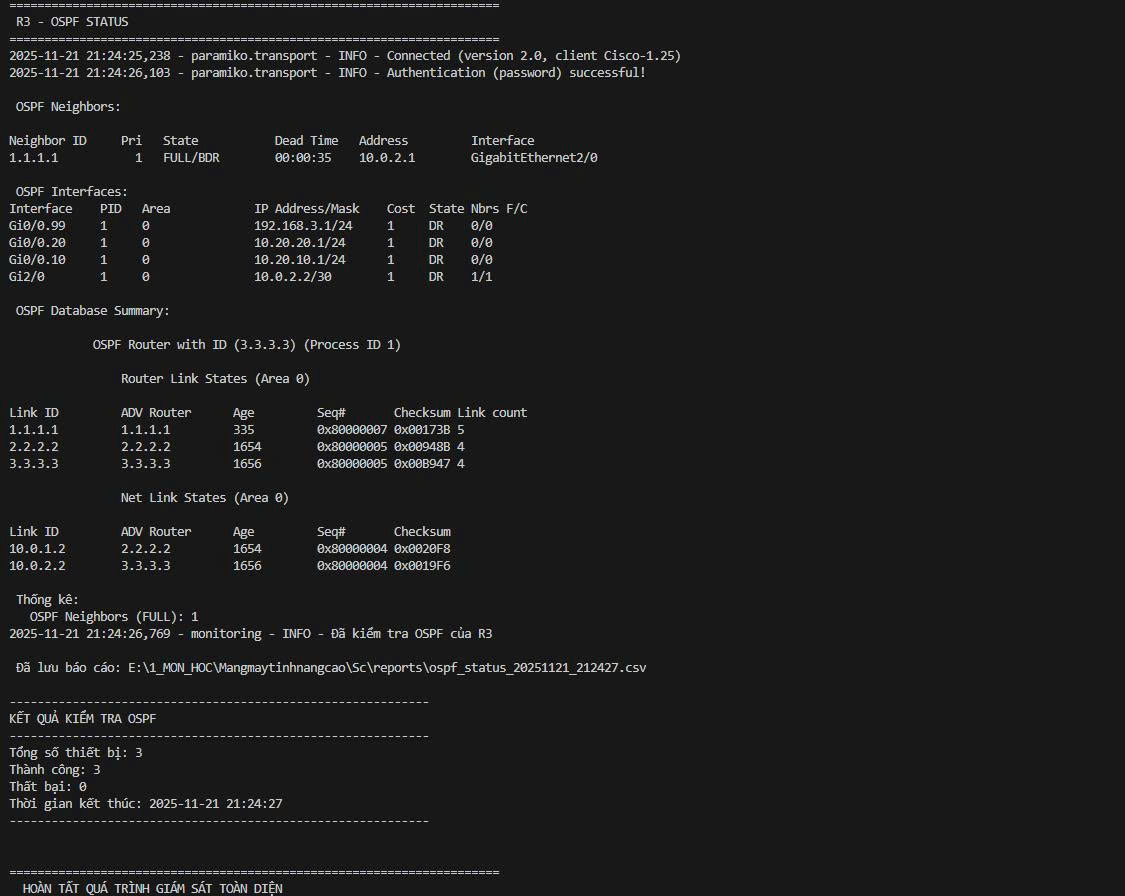
\includegraphics[width=0.7\textwidth]{image/mn_15.jpg}
        \caption{Kiểm tra trạng thái OSPF}
    \end{figure} % Bắt buộc phải có lệnh này
	\newpage \clearpage

    \section*{CHƯƠNG 6 - KẾT LUẬN}
\addcontentsline{toc}{section}{\numberline{}CHƯƠNG 6 -  KẾT LUẬN}
\setcounter{section}{6}
\setcounter{subsection}{0}
\setcounter{figure}{0}
\setcounter{table}{0}

%-------------Phần trình bày nội dung chương 6
Đề tài này đã thành công trong việc xây dựng một hệ thống tự động hóa quản lý và cấu hình mạng doanh nghiệp hoàn chỉnh, sử dụng ngôn ngữ lập trình Python kết hợp với thư viện Netmiko để tương tác với các thiết bị mạng được mô phỏng trên nền tảng GNS3-VM. Đây không chỉ là một bài tập học thuật đơn thuần, mà là một minh chứng rõ ràng cho thấy khả năng áp dụng công nghệ tự động hóa vào môi trường thực tế của doanh nghiệp hiện đại. Hệ thống đã được thiết kế với kiến trúc modular, cho phép dễ dàng bảo trì, mở rộng và tùy chỉnh theo nhu cầu cụ thể của từng tổ chức.

Về mặt kỹ thuật, đề tài đã triển khai thành công nhiều chức năng quan trọng trong quản lý mạng. Hệ thống có khả năng tự động hóa hoàn toàn quy trình cấu hình VLAN cho các Switch, bao gồm việc tạo VLAN, đặt tên và cấu hình các port ở chế độ trunk hoặc access. Đối với các Router, chương trình tự động gán địa chỉ IP cho các interface và subinterface, cấu hình encapsulation dot1q, và kích hoạt các interface một cách có hệ thống. Đặc biệt, việc thiết lập giao thức định tuyến OSPF được thực hiện tự động, bao gồm cấu hình router-id, quảng bá các network vào OSPF area, và kiểm tra trạng thái neighbor sau khi cấu hình. Tất cả các thao tác này được thực hiện thông qua việc gửi các lệnh CLI đến thiết bị qua giao thức SSH, nhờ vào khả năng của thư viện Netmiko trong việc mô phỏng tương tác con người với thiết bị mạng.

Một trong những điểm nổi bật của hệ thống là chức năng Backup và Restore thông minh. Chương trình có khả năng tự động sao lưu cấu hình của tất cả thiết bị với timestamp rõ ràng, giúp dễ dàng theo dõi lịch sử thay đổi cấu hình. Hệ thống lưu trữ file backup theo định dạng hostname\_backup\_YYYYMMDD\_HHMMSS.txt, cho phép quản lý và tra cứu nhanh chóng. Khi cần khôi phục, người dùng có thể chọn từ danh sách các file backup có sẵn, và hệ thống sẽ tự động làm sạch cấu hình bằng cách loại bỏ các dòng comment và metadata không cần thiết, sau đó áp dụng cấu hình theo từng batch để tránh tình trạng quá tải. Đặc biệt, chức năng mô phỏng lỗi và tự động khôi phục đã chứng minh tính ổn định và độ tin cậy của hệ thống, khi chương trình có thể phát hiện và khôi phục cấu hình một cách tự động mà không cần sự can thiệp của con người.

Hệ thống giám sát được tích hợp trong dự án cung cấp khả năng theo dõi trạng thái mạng một cách toàn diện. Chương trình có thể kiểm tra kết nối SSH đến tất cả thiết bị, đo thời gian phản hồi và kiểm tra uptime của từng thiết bị. Đối với interface, hệ thống tự động thu thập thông tin về trạng thái up/down, địa chỉ IP được gán và các thông số kỹ thuật khác. Trên các Router, chương trình giám sát bảng định tuyến, kiểm tra các route được học qua OSPF hoặc static route, và đánh giá tình trạng kết nối giữa các router trong mạng OSPF. Đối với Switch, hệ thống theo dõi cấu hình VLAN, trạng thái các trunk port và phân bổ VLAN trên từng access port. Tất cả thông tin giám sát này được ghi nhận vào file log chi tiết và tạo báo cáo dưới dạng CSV để phục vụ cho việc phân tích và báo cáo định kỳ.

GNS3-VM đóng vai trò là nền tảng mô phỏng mạnh mẽ trong dự án này, cho phép tạo ra một môi trường mạng doanh nghiệp phức tạp mà không cần đầu tư vào thiết bị phần cứng đắt tiền. Khác với các simulator đơn giản như Packet Tracer, GNS3 sử dụng các IOS image thực của Cisco, mang lại trải nghiệm gần giống với môi trường production. Điều này đặc biệt quan trọng vì nhiều tính năng và hành vi của thiết bị thực không được mô phỏng chính xác trên các simulator giản lược. GNS3-VM tích hợp tốt với Python thông qua giao thức SSH, cho phép các script tự động có thể kết nối và điều khiển thiết bị từ xa một cách linh hoạt. Môi trường ảo hóa này cũng giúp tiết kiệm đáng kể chi phí điện năng và không gian vật lý so với việc vận hành một lab với thiết bị thật, đồng thời cho phép dễ dàng snapshot và rollback khi cần thiết.
    
	\newpage \clearpage
	% --- TÀI LIỆU THAM KHẢO ---
	\phantomsection
    \addcontentsline{toc}{section}{TÀI LIỆU THAM KHẢO} 
    \bibliography{tailieuthamkhao} 
    \newpage
	
	% \input{appendix} % Phụ lục
	
\end{document}